%
% Apêndices
%

\chapter{\textit{p}Nota}
\label{manual-pNota}

De forma descritiva, apresentamos aqui detalhes do código do \textit{p}Nota separado em duas partes. Uma referente ao particionamento e aquisição de padrões e outra ao desenvolvimento e modeagem do critério avaliativo, ambos demonstrados através dos parâmetros e das resultantes obtidas pelo sistema. Assim, vamos separar nestas duas partes, a requisição de anotação do processo em \textit{main\_clustering.py} e a avaliação e produção de \textit{feedbacks} em \textit{main\_classification.py}.

\section{\textit{main\_clustering.py}}

Este é o processo que envolve a \textit{clusterização} e a seleção de itens para partições de treino e teste. Os parâmetros do processo incluem:


\texttt{
\begin{itemize}
    \scriptsize
\item (\textit{p}Nota\_module) [args] <dataset\_dir>
\item \textbf{dataset\_dir:}
    \subitem Caminho para a pasta do dataset.
\item \textbf{help: --help ou -h.}
    \subitem Descrição e ajuda.
\item \textbf{data\_structure: --dbstructure ou -s.}
    \subitem Modelo de arquivo(s) do dataset
    \subitem Default: moodle\_files. [ moodle\_files, single\_file, just\_files]
\item \textbf{data\_file: --filename ou -f.}
    \subitem Arquivo de entrada de respostas.
    \subitem Default: resposta.txt
\item \textbf{train\_document: --trdoc ou -d.}
    \subitem Arquivo de entrada de notas.
    \subitem Default notastreino.csv
\item \textbf{encoding: --encoding ou -e.}
    \subitem Padrão de caracteres.
    \subitem Default: utf-8. [ utf-8, iso-8859-1 ]
\item \textbf{n\_clusters: --nclusters ou -k.}
    \subitem Valor pré-fixado de clusters ou uso de otimização.
    \subitem Default: 0 (use optimization)
\item \textbf{train\_method: --trmethod ou -t.}
    \subitem Percentual da partição de treino.
    \subitem Default: 30
\item \textbf{language: --language ou -l.}
    \subitem Linguagem de entrada dos dados.
    \subitem Default: portuguese. [ portuguese, english, spanish ]
\item \textbf{enable\_container: --container ou -c.}
    \subitem Usar o modelo de container com Docker para processamento\footnote{Clustering-Optimization. Disponível em https://github.com/marcosspalenza/clustering\_optimization}.
    \subitem Default: enabled. [ enabled, disabled ]
\item \textbf{enable\_WordSTD: --wordmod ou -w.}
    \subitem Usar stemming ou lemmatization na transformação do texto.
    \subitem Default: stemm. [ stemm, lemma, none ]
\item \textbf{enable\_POS: --pos ou -p.}
    \subitem Usar Part-Of-Speech Tags na transformação do texto.
    \subitem Default: enabled. [ enabled, disabled ]
\item \textbf{enable\_NER: --ner ou -n.}
    \subitem Usar Named Entity Recognition na transformação do texto.
    \subitem Default: enabled. [ enabled, disabled ]
\item \textbf{enable\_MORPH: --morph ou -m.}
    \subitem Usar análise morfológica na transformação do texto.
    \subitem Default: enabled. [ enabled, disabled ]
\item \textbf{ignore\_clusters: --ignore\_clusters ou -i.}
    \subitem Ignorar qualquer resultado de clusterização prévia e reiniciar o processo.
    \subitem Default: disabled. [ enabled, disabled ]
\item \textbf{ngram\_start: --ngram\_start ou -x.}
    \subitem N-gram inicial para análise de sequencias textuais.
    \subitem Default: 1
\item \textbf{ngram\_end: --ngram\_end ou -x.}
    \subitem N-gram final para análise de sequencias textuais.
    \subitem Default 1
\item \textbf{generate\_reports: --generate\_reports ou -r.}
    \subitem Gerar relatórios ao final do processo.
    \subitem Default: enabled. [ enabled, disabled ]
\end{itemize}
}
As resultantes desta etapa de processamento são:

\texttt{
\begin{itemize}
    \scriptsize
\item data.mtx - Matriz de vetores no formato esparso Matrix Market.
\item doclist.mtx - Lista de identificadores dos documentos vetorizados.
\item wordlist.txt - Lista de características extraídas e seu peso após a vetorização.
\item Arquivos de \textit{clusterização}:
    \subitem exec.csv - Cada resultado do teste de parâmetros da clusterização.
    \subitem exceptions.csv - Cada teste de parâmetros que apresentou algum tipo de exceção.
    \subitem clusters.txt - Todos os índices de cluster resultantes de clusterização dos testes completos.
    \subitem cluster\{Id\}.txt - particionamento do resultado selecionado em arquivos individuais de índices de cluster com o grau de similaridade encontrado.
    \subitem clstr.cfg - configurações de clusterização selecionadas pelo método de ranking.
\item Arquivos de particionamento
    \subitem train - Lista de índices selecionados para anotação.
    \subitem test - Lista de índices selecionados para avaliação automática.
    \subitem minmax.mat - Lista de pares de amostras e o respectivo método de seleção adotado.
\item Relatórios
    \subitem Lista de respostas.
    \subitem Distribuição de clusters.
    \subitem Lista de amostras.
    \subitem Lista de características (ocorrência máxima e mínima).
    \subitem Relatório do padrão de respostas.
    \subitem Relatório da amostragem.
    \subitem Macros.
\item pNota.log - Logs do sistema.
\item notastreino.csv - Lista de índices dos documentos, nota atual e requisição \# de anotação.
\end{itemize}
}

Ao fim desta etapa a atividade contém informações de particionamento e a requisição de amostras para anotação. Além disso, parte dos relatórios são aqui gerados para apresentar, caso necessário, a etapa ao qual o processo se encontra. Inclusive, cada arquivo indica o estágio de desenvolvimento do processo e se a etapa foi corretamente executada.

\section{\textit{main\_classification.py}}

Este é o processo que envolve a classificação e a produção de \textit{feedbacks} como resultado. Os parâmetros do processo incluem:

\texttt{
\begin{itemize}
    \scriptsize
\item (\textit{p}Nota\_module) [args] <dataset\_dir>
\item \textbf{dataset\_dir:}
    \subitem Caminho para a pasta do dataset.
\item \textbf{help: --help ou -h.}
    \subitem Descrição e ajuda.
\item \textbf{data\_structure: --dbstructure ou -s.}
    \subitem Modelo de arquivo(s) do dataset
    \subitem Default: moodle\_files. [ moodle\_files, single\_file, just\_files]
\item \textbf{data\_file: --filename ou -f.}
    \subitem Arquivo de entrada de respostas.
    \subitem Default: resposta.txt
\item \textbf{train\_document: --trdoc ou -d.}
    \subitem Arquivo de entrada de notas.
    \subitem Default notastreino.csv
\item \textbf{encoding: --encoding ou -e.}
    \subitem Padrão de caracteres.
    \subitem Default: utf-8. [ utf-8, iso-8859-1 ]
\item \textbf{language: --language ou -l.}
    \subitem Linguagem de entrada dos dados.
    \subitem Default: portuguese. [ portuguese, english, spanish ]
\item \textbf{grade\_model: --grades ou -g.}
    \subitem Padrão de atribuição de notas do ambiente.
    \subitem Default: discrete. [ ordinal, discrete, continuous ]
\item \textbf{apply\_grader: --apply\_grader ou -a.}
    \subitem Permitir a avaliação para todas as amostras, inclusive os requisitos de anotação.
    \subitem Default: disabled. [ enabled, disabled ]
\item \textbf{individual\_reports: --individual\_reports ou -i.}
    \subitem Habilitar a criação de feedbacks individuais.
    \subitem Default: disabled. [ enabled, disabled ]
\end{itemize}
}

As resultantes desta etapa de processamento são:

\texttt{
\begin{itemize}
    \scriptsize
\item Resultados
    \subitem \{clf\}.labels - Lista de predições realizadas pelo classificador.
    \subitem \{clf\}.performance - Qualidade obtida em cada métrica.
\item Relatórios
    \subitem Marcações de resposta e correlação.
    \subitem Matriz de confusão.
    \subitem Gráfico de qualidade dos resultados.
    \subitem Quadro de rubrics.
    \subitem Regras da Decision Tree (modelo simplificado).
\item pNota.log - Logs do sistema.
\item notastreino.csv - Lista de índices dos documentos, notas e feedbacks.
\end{itemize}
}

Ao final deste processo são obtidas as notas e \textit{feedbacks} para discussão dos resultados e revisão da avaliação com o \textit{p}Nota. Se a etapa inicial foi efetivamente completa e as notas não foram corretamente geradas, o sistema aguarda até que tudo esteja de acordo para a produção de notas. Isso inclui esperar que todas as notas requisitadas sejam avaliadas ou que algum arquivo que não consta na lista seja criado. Portanto, nesta etapa a produção de notas envolve que tudo esteja de acordo com os pré-requisitos para execução bem como com os procedimentos anteriores.


\chapter{Exemplo}
\label{anexo-exemplo}

Para exemplificar o material produzido como resultados, \textit{feedbacks} e relatórios do \textit{p}Nota utilizamos uma questão da \textit{Open University} denominada \textit{Sandstone}. Essa questão foi selecionada pela diferença que a presença das palavras \textit{wind}, \textit{waves} e \textit{rivers} faz segundo o critério avaliativo. As respostas que descreviam a formação da \textit{sandstone}, ou arenito, por meio destas ações do meio sobre as particulas sedmentares foram avaliados como correto - 1. Por outro lado, não mencionar esse processo de formação resultava em nota 0. Abaixo apresentamos o enunciado da questão selecionada e a expectativa de resposta:

\blockquote{
	Sandstone is a medium-grained sedimentary rock. It is pale yellow, grey or often red to brown. Composed of rounded grains of silica (quartz) that are all the same size, it is cemented together by silica, calcite or an iron mineral.

	Sandstones are often layered and can show colour variations between the layers.

	How is it formed?

	Sand sized grains of quartz are produced by the weathering of other rocks. These are transported and deposited by wind, waves and rivers. The original sediment may have been a sand bank, beach or desert sand dunes.

	When the sand is buried beneath other sediments it is compacted and cemented by chemicals dissolved in the water seeping through it. Sandstones formed in deserts are usually red in colour. Those formed on beaches or rivers are often yellow or grey.
}

\begin{landscape}
\section{Lista de Respostas}

A lista de respostas é a apresentação do conteúdo do \textit{dataset} no relatório. Nele estão os identificadores do estudante, a nota recebida (se atribuída) e a resposta dada para a questão. A Tabela \ref{exemplo-respostas} apresenta uma parte do relatório com 50 das respostas do conjunto.

\begin{center}  
\scriptsize
\begin{longtable}{p{5cm} p{3cm} p{12cm}} \\ \hline 
         Id & Nota & Resposta \\ \hline  
         \endhead  
         \hline  
         \multicolumn{3}{r}{Continua na pr{\'o}xima p{\'a}gina} \\  
         \endfoot  
         \hline \hline  
         \multicolumn{3}{r}{{\'U}ltima p{\'a}gina} \\
         \caption{Amostra de parte do relatório com 50 respostas extraídas da atividade exemplo.}
         \label{exemplo-respostas} 
         \endlastfoot  

A249457X & 0.0 & this sand in this rock originally was located in a desert in oxidising conditions. 
 \\ \cline{2-3}

A249457X & 0.0 & this sand in this rock originally was located in a desert in oxidising conditions. 
 \\ \cline{2-3}

A249457X & 1.0 & this sand in this rock originally was located in a hot region in windy oxidising conditions. 
 \\ \cline{2-3}

A2548811 & 1.0 & it is most likely to have formed under arid desert conditions and transported by air and wind 
 \\ \cline{2-3}

T0632747 & 1.0 & sedimentary oxidised desert sandstone well weathered from strong winds 
 \\ \cline{2-3}

Y9003030 & 0.0 & from a desert and blown by the wind. once oxidising conditions where iron sulfide oxidised.maybe from humid conditions 
 \\ \cline{2-3}

A3345548 & 1.0 & reddened suggests desert. wellsorted fine pitted suggests blown and deposited by wind. wellrounded suggests possibly a dune. 
 \\ \cline{2-3}

U0991840 & 0.0 & the rock was formed in a gradually slowing current and have been exposed to oxidising conditions 
 \\ \cline{2-3}

U0991840 & 1.0 & there has been wind erosion and oxidised iron and have then been rounded and deposited in a gradual current. 
 \\ \cline{2-3}

Y8831914 & 0.0 & this rock layers together by the sand and grains of preexisting rocks of different size shape to form sandstone 
 \\ \cline{2-3}

Y8831914 & 0.0 & sandstone is a rock sedimentary which contain rocks and sand layered together. 
 \\ \cline{2-3}

Y8831914 & 0.0 & sandstone is a rock sedimentary which contain rocks and sand layered together which mean that transported by weathering. 
 \\ \cline{2-3}

A2415177 & 1.0 & weathered quartz grains from a granite containing iron carried by wind in a desert. 
 \\ \cline{2-3}

X0816556 & 0.0 & not deposited slowly deposition from air 
 \\ \cline{2-3}

X0816556 & 0.0 & deposition from air the grains contain some iron oxid 
 \\ \cline{2-3}

Y6544188 & 0.0 & the presence of reddned grains shows that sandstone derivates from sediments. sandstone is a sedimentary rock. 
 \\ \cline{2-3}

Y6544188 & 0.0 & the rock is sedimentary in origin. 
 \\ \cline{2-3}

Y6544188 & 0.0 & the sandstone was formed by deposition of flowing water. the reddened grains shows that sanstone is rich in oxygen. 
 \\ \cline{2-3}

A2482988 & 0.0 & it came from a higher class of diy store probably one of the quality garden centres squires rather than bq. 
 \\ \cline{2-3}

A2482988 & 0.0 & rolling down river of iron oxide weathering sedimentary clastic rocks full of hyrothermal fluids 
 \\ \cline{2-3}

A2482988 & 0.0 & the question is about the origins not the mode of transport as to how they got where they are. 
 \\ \cline{2-3}

A1424820 & 0.0 & this rock originated in an arid desert environment that allowed physical erosion of sediments in highly oxidising conditions. 
 \\ \cline{2-3}

A1424820 & 1.0 & this sandstone originated in a desert environment with wind blown physical weathering of mineral grains in highly oxidising conditions. 
 \\ \cline{2-3}

A2843422 & 0.0 & the sandstone would have formed and originated in desert conditions as part of desert sands. 
 \\ \cline{2-3}

A2843422 & 0.0 & the sandstone would have originated in the desert. 
 \\ \cline{2-3}

A2843422 & 1.0 & the sandstone would have originated in the desert as part of a windblown dune. 
 \\ \cline{2-3}

Y762039X & 0.0 & that the sandstone originated from a desert 
 \\ \cline{2-3}

Y762039X & 0.0 & originated from a sand desert. 
 \\ \cline{2-3}

Y762039X & 0.0 & originated from dunes in a sand desert. 
 \\ \cline{2-3}

Y3512671 & 1.0 & desert sandstone experiencing high oxidising conditions transported by wind 
 \\ \cline{2-3}

Y6523161 & 0.0 & called a conglomerate and sedimentary in construction broken by weathering erosion transport and finally deposited. 
 \\ \cline{2-3}

Y6523161 & 0.0 & were there before uncomformity occurred then weathering and erosion took place 
 \\ \cline{2-3}

Y6523161 & 1.0 & grains were wind transported and were oxidised under humid conditions 
 \\ \cline{2-3}

A3317409 & 0.0 & transported through water 
 \\ \cline{2-3}

A3317409 & 0.0 & tha sandstone is made from sediment transported through water to its resting place. 
 \\ \cline{2-3}

A3317409 & 0.0 & tha sandstone is made from sediment transported through water to its resting place. 
 \\ \cline{2-3}

Y8696943 & 0.0 & it was most likely to have formed under desert conditions 
 \\ \cline{2-3}

Y8696943 & 1.0 & originated as desert sandblown by wind and undergone oxidisation 
 \\ \cline{2-3}

Y9311424 & 0.0 & snadstone was formed on dea bed that dried 
 \\ \cline{2-3}

Y9311424 & 0.0 & sandstone was formed from sediment that entered a river and deposited 
 \\ \cline{2-3}

Y9311424 & 0.0 & sandstone was formed from sediment that entered a river and deposited they were transported by water 
 \\ \cline{2-3}

Y8964340 & 1.0 & that it may of came from a windy desert environment 
 \\ \cline{2-3}

A2336136 & 0.0 & the rock originated in a hot dry climate such as a desert. 
 \\ \cline{2-3}

A2336136 & 0.0 & it is a desert sandstone. 
 \\ \cline{2-3}

A2336136 & 1.0 & it originates in a hot dry environment weathered and transported by wind. 
 \\ \cline{2-3}

X8581258 & 1.0 & these were desert grains moved by the wind finely pitted by repeated impacts and red from oxidised iron 
 \\ \cline{2-3}

Y1699145 & 1.0 & they would be wind blown desert sand formed in oxidising times like the devonian period. 
 \\ \cline{2-3}

Y8883735 & 1.0 & the grains have been moved by wind colliding with each other to become rounded and pitted with an iron coating. 
 \\ \cline{2-3}

Y8883735 & 1.0 & very chemically weathered and moved by wind. 
 \\ \cline{2-3}

Y8883735 & 1.0 & very chemically weathered and moved by wind and exposed to oxidising conditions. 
 \\ \cline{2-3}

 & \multicolumn{2}{r}{$ \hdots $  Foram omitidos os demais resultados (1897 respostas no total).} \\

\end{longtable}  
\end{center}


\section{Distribuição de \textit{Clusters}}

Com todas as respostas, o processo de \textit{clusterização} identifica padrões de associação e agrupa amostras em subgrupos, denominados \textit{clusters}. Apresentamos através da Tabela \ref{exemplo-clusters} o particionamento do conjunto de respostas e, em destaque, os itens selecionados para avaliação.

\begin{center}
\scriptsize
\begin{longtable}{p{2cm} p{2cm} p{16cm}} \\ \hline 
         Cluster & Tamanho & Itens \\ \hline 
         \endhead 
         \hline 
         \multicolumn{3}{r}{Continua na pr{\'o}xima p{\'a}gina} \\ 
         \endfoot 
         \hline \hline         \multicolumn{3}{r}{{\'U}ltima p{\'a}gina} \\ 
         \caption{Clusters formados com cada uma das respostas da atividade \textit{Sandstone}.}
         \label{exemplo-clusters}
         \endlastfoot

0 & 16 & 68 256 \textbf{353} \textbf{354} 390 513 695 \textbf{753} 754 1097 \textbf{1098} 1159 1231 1643 1843 1882 \\ \cline{3-3} 

1 & 8 & \textbf{246} \textbf{247} \textbf{265} \textbf{266} 356 \textbf{542} \textbf{1197} 1579 \\ \cline{3-3} 

2 & 461 & 13 16 24 \textbf{26} 27 28 33 36 \textbf{43} 48 50 \textbf{52} 57 58 59 60 61 63 69 70 71 73 75 76 78 79 \textbf{80} 82 92 93 95 96 99 100 101 107 110 \textbf{111} 117 118 129 136 137 138 159 161 162 165 166 167 170 171 172 173 176 177 178 179 182 188 189 190 194 206 222 231 241 242 252 254 257 261 262 264 276 277 278 285 291 299 \textbf{302} 303 304 315 \textbf{316} 319 322 325 331 339 340 341 345 \textbf{347} 348 361 362 363 367 368 369 370 391 392 393 402 405 \textbf{407} 424 428 429 436 439 440 452 453 \textbf{454} 471 475 480 485 490 \textbf{491} 497 498 500 501 502 504 505 511 516 517 518 523 \textbf{524} 527 528 536 537 \textbf{538} 539 550 556 559 562 570 572 576 581 \textbf{595} 602 607 608 \textbf{609} 612 613 615 616 617 \textbf{620} 628 630 632 634 639 640 641 650 662 672 673 \textbf{675} 678 \textbf{683} \textbf{685} 686 689 692 \textbf{704} 708 709 710 713 \textbf{714} 718 719 729 730 731 735 744 757 758 760 761 763 775 780 790 796 \textbf{797} 799 800 811 816 \textbf{821} 822 823 824 837 844 \textbf{845} 867 873 876 878 881 882 883 884 \textbf{890} 891 892 895 896 898 899 902 \textbf{903} 905 914 915 918 920 \textbf{922} \textbf{931} 946 956 967 969 970 973 975 981 982 994 1010 1011 1014 1021 1024 1027 1032 1048 1049 1050 1051 1053 1060 1062 1063 1064 1066 1067 1071 1072 1073 1075 1078 1082 1083 1084 1085 1086 1088 1099 \textbf{1102} 1106 1108 1109 1110 \textbf{1119} 1125 1128 1129 1130 \textbf{1131} 1132 1134 1135 1137 1138 1139 1141 1142 1143 1146 1152 1153 1156 \textbf{1157} 1166 1171 \textbf{1174} \textbf{1175} 1177 1187 \textbf{1188} 1192 1203 1208 \textbf{1210} 1218 1221 1224 1225 1228 1233 1234 1239 \textbf{1253} 1255 1258 1260 1268 1272 \textbf{1285} 1293 1294 \textbf{1301} 1305 1306 1319 1332 \textbf{1334} 1337 1341 1345 1353 1358 1360 1361 1366 1368 1372 1374 1380 1388 1395 1398 1400 1401 1402 \textbf{1403} 1404 1415 1430 1432 1443 1445 1450 1451 1452 1454 1457 1470 1473 1474 1475 \textbf{1478} 1481 \textbf{1483} \textbf{1485} 1491 1492 1501 1502 1511 1512 1514 1523 1528 1529 1537 1538 1543 1547 1548 1555 1558 \textbf{1566} \textbf{1570} 1572 1586 1587 1588 \textbf{1618} 1621 1625 1635 \textbf{1646} 1647 1651 1652 1662 1667 1670 1671 1677 1678 1683 1684 1686 1687 1688 1704 1705 1707 1716 \textbf{1717} 1721 1722 1729 1731 1736 1742 1743 1750 1753 1762 1770 1779 1781 1789 1790 1796 1797 1801 1802 1803 1806 \textbf{1808} \textbf{1811} \textbf{1812} 1820 1831 \textbf{1833} 1834 1835 1838 1851 \textbf{1858} 1876 1877 1880 1890 1891 \textbf{1892} 1893 \textbf{1894} \\ \cline{3-3} 

3 & 31 & 19 21 \textbf{120} \textbf{122} \textbf{288} 301 \textbf{379} 380 415 445 \textbf{451} \textbf{478} 506 512 \textbf{603} \textbf{604} 787 \textbf{802} 831 832 834 841 \textbf{916} 930 1020 1518 1576 1628 1673 1674 \textbf{1675} \\ \cline{3-3} 

4 & 12 & \textbf{86} \textbf{87} 109 342 \textbf{589} 1170 1223 1261 \textbf{1304} 1378 1696 1767 \\ \cline{3-3} 

5 & 24 & \textbf{269} \textbf{310} \textbf{326} 330 \textbf{371} 534 600 605 606 647 872 1195 1199 1236 1248 1265 \textbf{1510} \textbf{1596} 1597 \textbf{1608} 1617 1620 1739 1862 \\ \cline{3-3} 

6 & 50 & 45 62 \textbf{94} \textbf{126} \textbf{169} \textbf{196} \textbf{217} 230 320 \textbf{359} \textbf{377} \textbf{447} \textbf{448} 487 551 \textbf{590} 614 688 691 696 \textbf{771} \textbf{772} 838 863 \textbf{913} \textbf{988} \textbf{998} 1016 \textbf{1030} \textbf{1165} 1212 1283 1331 \textbf{1342} 1357 1399 1455 \textbf{1480} 1497 1562 1564 1627 1724 \textbf{1732} 1766 \textbf{1795} 1823 1860 1871 \textbf{1886} \\ \cline{3-3} 

7 & 20 & \textbf{5} \textbf{185} \textbf{410} \textbf{681} \textbf{769} 792 \textbf{803} \textbf{828} \textbf{848} \textbf{864} \textbf{963} \textbf{1004} \textbf{1022} \textbf{1183} \textbf{1184} \textbf{1207} \textbf{1591} \textbf{1637} 1741 \textbf{1824} \\ \cline{3-3} 

8 & 300 & \textbf{0} \textbf{1} 3 14 20 31 32 37 38 39 42 49 56 64 67 77 81 83 89 97 112 113 119 \textbf{131} 139 146 153 160 163 164 168 \textbf{183} 195 203 208 \textbf{211} 212 \textbf{214} \textbf{219} 221 224 229 232 233 235 236 \textbf{250} 258 263 270 272 282 290 \textbf{292} 293 295 300 312 321 324 328 329 332 335 338 344 350 \textbf{351} 360 364 365 372 382 383 395 396 404 \textbf{422} 427 434 441 \textbf{442} \textbf{461} 464 466 474 476 479 481 499 \textbf{520} 526 529 530 531 532 555 557 561 564 567 568 574 575 577 578 579 585 \textbf{591} \textbf{592} 593 598 618 624 625 631 637 638 649 658 659 660 661 665 674 676 682 690 693 705 706 715 720 721 \textbf{727} 737 738 750 762 764 765 781 \textbf{783} 793 798 807 808 809 812 814 817 825 826 827 877 887 889 897 900 904 912 921 925 929 938 940 947 948 951 961 \textbf{965} 968 971 \textbf{985} 1000 1002 1019 1026 1038 1044 \textbf{1045} 1046 1057 1059 1076 1087 1089 1090 \textbf{1101} 1113 1114 1123 1133 \textbf{1140} 1145 1158 1162 1167 1176 1178 1179 1182 1185 1186 1193 1209 1219 1222 1235 1240 1244 1249 1259 1282 1288 1295 1296 1299 1307 \textbf{1310} 1314 1315 \textbf{1316} 1321 1340 \textbf{1343} 1350 1352 1354 1359 1373 1379 1391 1406 1456 1471 1477 1482 \textbf{1484} 1488 1489 1493 1496 1503 1507 1521 \textbf{1559} 1560 1569 1577 1585 1589 1609 1610 1611 1613 1622 1623 1630 1636 1640 1653 1659 1663 1664 1668 1669 1672 1681 1685 1697 1699 1715 1719 1723 1725 1730 1746 1751 1755 1758 1761 1764 1771 1772 1775 \textbf{1776} 1782 \textbf{1785} 1786 1787 1791 1813 1821 1830 \textbf{1841} 1853 1856 1866 1879 \\ \cline{3-3} 

9 & 38 & 22 91 175 \textbf{220} 259 \textbf{398} \textbf{433} 449 \textbf{560} 565 \textbf{635} \textbf{656} 663 \textbf{747} 779 \textbf{861} 910 932 962 1006 1120 1164 \textbf{1267} 1298 1300 1347 \textbf{1365} \textbf{1431} 1440 1476 1542 \textbf{1565} \textbf{1599} 1601 \textbf{1602} \textbf{1676} \textbf{1777} 1896 \\ \cline{3-3} 

10 & 7 & \textbf{1148} \textbf{1238} \textbf{1439} 1441 \textbf{1448} 1495 1740 \\ \cline{3-3} 

11 & 37 & 90 181 287 336 384 521 657 664 698 \textbf{701} 702 703 \textbf{726} 743 751 \textbf{819} 840 \textbf{875} 907 911 987 1015 1052 1181 \textbf{1229} \textbf{1270} \textbf{1271} 1308 1309 1444 1527 1546 1594 1679 1744 1804 1867 \\ \cline{3-3} 

12 & 250 & 4 \textbf{7} 8 \textbf{10} \textbf{29} \textbf{34} \textbf{35} 40 44 53 72 74 \textbf{88} \textbf{98} \textbf{106} \textbf{114} \textbf{116} \textbf{124} 128 130 \textbf{135} 197 210 \textbf{218} 234 238 239 240 \textbf{251} \textbf{271} 273 \textbf{279} \textbf{280} 283 \textbf{314} 318 333 334 346 366 \textbf{376} 381 385 \textbf{389} \textbf{406} \textbf{411} \textbf{416} \textbf{418} \textbf{419} 425 \textbf{426} 437 438 468 \textbf{469} \textbf{470} \textbf{472} \textbf{482} \textbf{486} 488 \textbf{489} 509 \textbf{533} \textbf{540} 541 \textbf{563} \textbf{571} \textbf{580} 587 \textbf{596} \textbf{610} 611 619 \textbf{621} \textbf{626} \textbf{627} 636 \textbf{642} 644 \textbf{645} \textbf{646} 651 \textbf{652} \textbf{666} 679 \textbf{680} \textbf{687} 694 \textbf{711} 716 722 \textbf{728} 739 \textbf{740} \textbf{741} 742 759 766 \textbf{770} \textbf{776} \textbf{786} 801 804 820 \textbf{839} \textbf{842} \textbf{855} 856 \textbf{860} 888 \textbf{894} \textbf{901} 906 \textbf{919} 926 935 941 \textbf{955} 957 \textbf{976} \textbf{977} 990 \textbf{993} 1001 \textbf{1012} 1028 \textbf{1029} 1034 1040 \textbf{1041} \textbf{1054} 1068 1074 \textbf{1118} \textbf{1126} \textbf{1144} 1147 1149 \textbf{1150} 1161 \textbf{1168} 1169 1172 \textbf{1173} 1189 1204 1206 1215 1227 1245 \textbf{1252} \textbf{1256} \textbf{1269} 1275 1276 1287 \textbf{1289} \textbf{1302} \textbf{1303} 1318 1322 \textbf{1323} 1324 \textbf{1326} \textbf{1327} 1328 \textbf{1330} 1335 1336 \textbf{1338} 1339 \textbf{1346} \textbf{1349} 1356 \textbf{1362} \textbf{1363} 1367 \textbf{1370} 1371 \textbf{1384} \textbf{1385} \textbf{1386} \textbf{1390} \textbf{1394} \textbf{1411} \textbf{1417} 1418 \textbf{1422} \textbf{1426} 1437 \textbf{1453} 1459 1461 \textbf{1472} 1479 \textbf{1486} \textbf{1487} 1490 \textbf{1504} 1516 \textbf{1545} 1551 \textbf{1563} 1571 1573 \textbf{1575} \textbf{1581} 1582 1584 \textbf{1590} 1644 1648 \textbf{1656} 1658 \textbf{1666} 1695 \textbf{1702} \textbf{1708} \textbf{1709} 1713 1714 1718 1745 \textbf{1747} \textbf{1754} \textbf{1757} 1759 1768 1788 \textbf{1798} 1815 1816 \textbf{1817} 1818 1826 1828 \textbf{1836} \textbf{1837} \textbf{1839} \textbf{1840} \textbf{1845} 1847 \textbf{1857} 1859 \textbf{1863} \textbf{1872} \textbf{1883} \textbf{1884} 1885 1895 \\ \cline{3-3} 

13 & 3 & \textbf{156} \textbf{1499} \textbf{1784} \\ \cline{3-3} 

14 & 4 & \textbf{215} \textbf{846} \textbf{1263} 1278 \\ \cline{3-3} 

15 & 8 & 105 458 \textbf{974} 1023 1043 1421 \textbf{1424} \textbf{1425} \\ \cline{3-3} 

16 & 25 & \textbf{41} 142 202 \textbf{412} \textbf{413} \textbf{467} 588 \textbf{669} \textbf{697} 953 \textbf{992} 995 \textbf{1107} 1121 \textbf{1273} 1274 1297 \textbf{1344} \textbf{1393} 1405 1464 1469 \textbf{1567} \textbf{1612} 1692 \\ \cline{3-3} 

17 & 3 & \textbf{937} \textbf{1190} \textbf{1434} \\ \cline{3-3} 

18 & 84 & \textbf{51} 84 121 157 200 207 213 216 253 294 307 311 343 375 378 \textbf{394} 397 435 455 456 457 465 558 \textbf{573} 629 648 671 \textbf{677} 723 736 \textbf{745} 785 794 810 818 830 \textbf{843} 865 866 868 \textbf{870} 874 \textbf{917} \textbf{980} 1007 1008 1025 1031 1035 \textbf{1091} 1095 1112 1151 1154 1198 1202 1311 \textbf{1377} 1416 1429 \textbf{1460} 1494 \textbf{1498} 1515 1519 1524 1530 1549 1593 1604 1624 \textbf{1632} 1633 1634 1680 1690 1799 1807 1814 1822 1825 1870 1878 1889 \\ \cline{3-3} 

19 & 7 & \textbf{141} 192 \textbf{933} 1241 \textbf{1355} 1435 \textbf{1438} \\ \cline{3-3} 

20 & 10 & \textbf{226} \textbf{227} 403 584 \textbf{633} 724 986 1281 \textbf{1465} \textbf{1887} \\ \cline{3-3} 

21 & 20 & 191 \textbf{355} 601 712 939 954 1017 \textbf{1018} 1055 1081 1232 1442 1550 1598 \textbf{1710} \textbf{1711} \textbf{1712} \textbf{1760} 1800 1810 \\ \cline{3-3} 

22 & 75 & 23 25 144 154 \textbf{158} 174 186 193 225 296 \textbf{323} 337 401 \textbf{420} 423 430 \textbf{450} 463 483 \textbf{492} 493 503 \textbf{507} 522 \textbf{525} 543 544 670 746 \textbf{773} 782 \textbf{795} 829 \textbf{847} 871 885 \textbf{909} 942 943 964 \textbf{966} 972 1013 1093 1096 \textbf{1122} 1237 \textbf{1254} \textbf{1257} \textbf{1279} \textbf{1280} 1286 1312 1313 1333 1387 1420 \textbf{1433} 1500 1525 1533 1556 1629 1639 1641 \textbf{1682} 1693 1698 1749 1752 \textbf{1763} 1773 1809 1829 1854 \\ \cline{3-3} 

23 & 5 & 134 1033 \textbf{1375} \textbf{1376} \textbf{1408} \\ \cline{3-3} 

24 & 21 & \textbf{11} 55 \textbf{132} \textbf{133} \textbf{184} \textbf{260} \textbf{473} \textbf{699} \textbf{777} \textbf{778} \textbf{789} \textbf{833} \textbf{853} 1111 1117 \textbf{1160} \textbf{1194} \textbf{1205} 1214 1508 1881 \\ \cline{3-3} 

25 & 3 & \textbf{1036} \textbf{1116} \textbf{1727} \\ \cline{3-3} 

26 & 10 & 459 462 \textbf{566} 1005 \textbf{1213} 1436 \textbf{1531} \textbf{1848} \textbf{1849} 1850 \\ \cline{3-3} 

27 & 4 & \textbf{102} \textbf{508} \textbf{1039} 1262 \\ \cline{3-3} 

28 & 8 & \textbf{373} \textbf{547} \textbf{732} 791 \textbf{813} \textbf{862} \textbf{1211} \textbf{1700} \\ \cline{3-3} 

29 & 2 & \textbf{858} \textbf{1247} \\ \cline{3-3} 

30 & 2 & \textbf{1615} \textbf{1616} \\ \cline{3-3} 

31 & 9 & \textbf{127} \textbf{248} \textbf{249} \textbf{317} \textbf{399} 806 1544 \textbf{1650} 1793 \\ \cline{3-3} 

32 & 4 & \textbf{755} \textbf{1592} \textbf{1603} \textbf{1769} \\ \cline{3-3} 

33 & 15 & \textbf{15} 17 66 103 \textbf{104} 400 \textbf{1216} \textbf{1217} 1226 1290 \textbf{1291} 1389 1535 \textbf{1536} 1649 \\ \cline{3-3} 

34 & 2 & \textbf{6} \textbf{1557} \\ \cline{3-3} 

35 & 16 & 201 \textbf{274} 281 408 414 583 774 854 \textbf{927} \textbf{928} 997 \textbf{1047} 1277 \textbf{1583} \textbf{1774} \textbf{1868} \\ \cline{3-3} 

36 & 81 & 125 143 145 148 \textbf{152} 155 187 237 275 284 286 289 297 305 352 421 431 \textbf{460} 484 494 546 549 569 594 \textbf{667} 717 752 788 \textbf{835} \textbf{836} 852 857 \textbf{879} 893 936 1003 1042 1058 1065 1077 \textbf{1094} 1100 1104 1105 1115 1155 \textbf{1180} 1191 1329 \textbf{1369} 1381 1382 1412 1428 1449 1458 1466 1468 1506 1509 1513 1532 1561 1578 1606 \textbf{1631} 1638 1657 1689 1691 1703 \textbf{1733} 1734 \textbf{1735} 1738 1765 1780 1794 1805 1842 1869 \\ \cline{3-3} 

37 & 1 & \textbf{999} \\ \cline{3-3} 

38 & 11 & \textbf{386} \textbf{387} \textbf{388} \textbf{409} \textbf{432} 653 \textbf{654} 700 \textbf{1246} \textbf{1383} \textbf{1855} \\ \cline{3-3} 

39 & 2 & \textbf{748} \textbf{749} \\ \cline{3-3} 

40 & 8 & \textbf{9} 228 \textbf{327} \textbf{1243} \textbf{1266} 1410 \textbf{1778} 1846 \\ \cline{3-3} 

41 & 1 & \textbf{495} \\ \cline{3-3} 

42 & 4 & \textbf{869} \textbf{1325} \textbf{1520} 1832 \\ \cline{3-3} 

43 & 1 & \textbf{309} \\ \cline{3-3} 

44 & 1 & \textbf{1720} \\ \cline{3-3} 

45 & 5 & \textbf{180} 934 \textbf{1136} \textbf{1397} \textbf{1407} \\ \cline{3-3} 

46 & 9 & \textbf{519} 944 \textbf{949} \textbf{989} \textbf{1127} 1264 1522 1541 1568 \\ \cline{3-3} 

47 & 2 & \textbf{18} \textbf{960} \\ \cline{3-3} 

48 & 2 & \textbf{622} \textbf{1827} \\ \cline{3-3} 

49 & 6 & \textbf{198} \textbf{199} \textbf{245} \textbf{1554} 1655 1861 \\ \cline{3-3} 

50 & 1 & \textbf{859} \\ \cline{3-3} 

51 & 76 & 12 47 85 108 115 123 \textbf{149} \textbf{150} \textbf{151} \textbf{204} 205 223 244 306 313 349 417 446 535 545 \textbf{552} 553 554 582 586 599 643 684 725 \textbf{733} 815 \textbf{880} 923 \textbf{924} 945 978 996 1009 1056 1061 1069 \textbf{1070} 1103 1163 \textbf{1196} 1200 1242 1284 1292 1320 \textbf{1364} 1413 \textbf{1414} 1419 1427 1447 1462 \textbf{1463} 1467 1526 \textbf{1553} \textbf{1607} 1619 1654 \textbf{1660} \textbf{1726} 1728 1748 \textbf{1756} 1783 1792 1819 \textbf{1852} 1864 \textbf{1865} 1873 \\ \cline{3-3} 

52 & 3 & \textbf{444} \textbf{983} \textbf{1505} \\ \cline{3-3} 

53 & 15 & 30 46 \textbf{140} \textbf{147} 243 597 707 \textbf{756} 1201 1351 \textbf{1446} 1600 \textbf{1665} \textbf{1694} \textbf{1888} \\ \cline{3-3} 

54 & 43 & 2 54 \textbf{209} 298 357 \textbf{374} 477 510 548 623 655 734 767 \textbf{768} 784 \textbf{805} 849 \textbf{850} \textbf{851} 886 \textbf{950} 958 959 979 991 1037 1079 \textbf{1080} \textbf{1124} 1317 1348 1392 1539 \textbf{1540} 1580 \textbf{1595} 1626 \textbf{1642} 1645 1661 1844 \textbf{1874} 1875 \\ \cline{3-3} 

55 & 6 & 443 \textbf{496} \textbf{514} \textbf{984} \textbf{1396} \textbf{1701} \\ \cline{3-3} 

56 & 1 & \textbf{1574} \\ \cline{3-3} 

57 & 3 & \textbf{515} \textbf{1230} \textbf{1614} \\ \cline{3-3} 

58 & 21 & \textbf{65} 255 \textbf{267} \textbf{268} 308 358 668 \textbf{908} 952 \textbf{1092} 1220 \textbf{1250} 1251 1409 1423 1517 1534 1552 \textbf{1605} 1706 \textbf{1737} \\ \cline{3-3} 
\end{longtable}
\end{center}

\newpage

\section{Lista de Amostras por \textit{Cluster}}

Com um processo amostral que combinando diferentes modos, descrevemos através de cada amostra selecionada a técnica que foi aplicada. Isso por conta de que a técnica define detalhes da representatividade de cada amostra ao \textit{cluster} de origem, até o inicio da amostragem por distribuição. Assim, na Tabela \ref{exemplo-amostras} descrevemos o modo de amostragem adotado para as amostras de alguns dos \textit{clusters} da atividade \textit{Sandstone}.

\begin{center} 
\scriptsize
\begin{longtable}{p{2cm} p{2cm} p{2cm} p{14cm}} \\ \hline 
         Cluster & Id & M{\'e}todo & Resposta \\ \hline 
         \endhead 
         \hline 
         \multicolumn{4}{r}{Continua na pr{\'o}xima p{\'a}gina} \\ 
         \endfoot 
         \hline \hline         \multicolumn{4}{r}{{\'U}ltima p{\'a}gina} \\ 
         \caption{Seleção de amostras aplicada para a atividade \textit{Sandstone}.}
         \label{exemplo-amostras}
         \endlastfoot

0 & 353 & maxsim & the sandstone was probably formed in a desert or low energy environment- reddened grains suggests oxidisation of iron took place. \\ \cline{3-4}
0 & 753 & maxsim & southwest of england and wales- iron oxide from southwestern united states. quartz arenites. \\ \cline{3-4}
0 & 353 & minsim & the sandstone was probably formed in a desert or low energy environment- reddened grains suggests oxidisation of iron took place. \\ \cline{3-4}
0 & 354 & minsim & the sandstone was originally a beach or similar low energy environment- reddened grains suggests oxidisation of iron took place. \\ \cline{3-4}
0 & 753 & minsize & southwest of england and wales- iron oxide from southwestern united states. quartz arenites. \\ \cline{3-4}
0 & 354 & maxsize & the sandstone was originally a beach or similar low energy environment- reddened grains suggests oxidisation of iron took place. \\ \cline{3-4}
0 & 1098 & silhcoeff & the sandstone is transported by wind- originated in oxygen rich atmosphere is chemically weathered and transported in high energy conditions. \\ \cline{3-4}
1 & 1197 & maxsim & igneous rock-formed deep within earth and cooled slowly.mainly quartz-chemically weathered- longer aeolian processed-desert enviroment \\ \cline{3-4}
1 & 542 & maxsim & sandstone is a sedimentary rock composed mainly of sand-size mineral or rock grains. \\ \cline{3-4}
1 & 246 & minsim & it would have orriganated in a dessert because there reddened grains. it would have been deposited by slow moving water. \\ \cline{3-4}
1 & 247 & minsim & it would have orriganated in a dessert because there reddened grains. it would have been deposited by slow moving water. \\ \cline{3-4}
1 & 265 & minsize & the sandstone indicates continued hot- oxidising conditions and from a sedimentary origin. \\ \cline{3-4}
1 & 1197 & maxsize & igneous rock-formed deep within earth and cooled slowly.mainly quartz-chemically weathered- longer aeolian processed-desert enviroment \\ \cline{3-4}
1 & 266 & silhcoeff & the sandstone indicates continued hot- oxidising conditions and layered. so therefore from a sedimentary origin. \\ \cline{3-4}
2 & 845 & maxsim & well sorted and deposited by a current that gradually slowed by sediment slowing \\ \cline{3-4}
2 & 43 & maxsim & it is a desert sandstone. \\ \cline{3-4}
2 & 26 & minsim & that the sandstone originated from a desert \\ \cline{3-4}
2 & 111 & minsim & that the sandstone originated in the desert \\ \cline{3-4}
2 & 302 & minsize & weathered \\ \cline{3-4}
2 & 845 & maxsize & well sorted and deposited by a current that gradually slowed by sediment slowing \\ \cline{3-4}
2 & 1858 & silhcoeff & it is a sedimentary rock formed from grains from an arid desert \\ \cline{3-4}
2 & 1618 & silhcoeff & the sandstone grains originated in an arid desert. \\ \cline{3-4}
2 & 1485 & silhcoeff & the sandstone formed from ancient desert deposits. \\ \cline{3-4}
2 & 1174 & silhcoeff & this sandstone has actually originated from a rock in a desert. \\ \cline{3-4}
2 & 1119 & silhcoeff & the deposited sand originates from an ancient desert. \\ \cline{3-4}
2 & 52 & silhcoeff & this indicates it may be desert sandstone formed by the wind \\ \cline{3-4}
2 & 538 & silhcoeff & it originated from and area where iron was present in a river. \\ \cline{3-4}
2 & 347 & silhcoeff & the rock is from weathering which has produced a sedimentary rock. \\ \cline{3-4}
2 & 1570 & silhcoeff & the rock originated in the desert and was blown by the wind. \\ \cline{3-4}
2 & 714 & silhcoeff & it was probably transported by wind in desert conditions. \\ \cline{3-4}
2 & 1301 & silhcoeff & the rock is made from sand grains from the desert. \\ \cline{3-4}
2 & 620 & silhcoeff & the grains came from a desert sand dune. \\ \cline{3-4}
2 & 524 & silhcoeff & this rock appears to have its origin in desert sands. \\ \cline{3-4}
2 & 454 & silhcoeff & desert sand dunes sorted by wind. \\ \cline{3-4}
2 & 903 & silhcoeff & it indicates the origin is arid desert conditions. \\ \cline{3-4}
2 & 1157 & silhcoeff & it formed on land in arid conditions and was transported by wind \\ \cline{3-4}
2 & 1566 & silhcoeff & these indicators signify desert conditions in the past. \\ \cline{3-4}
2 & 1403 & silhcoeff & this is from the desert in origin it is windblown and formed on a dune. \\ \cline{3-4}
2 & 1894 & silhcoeff & the rock originates from ancient desert deposits. \\ \cline{3-4}
2 & 407 & silhcoeff & the sand was deposited as layers of an ancient desert. \\ \cline{3-4}
2 & 80 & silhcoeff & formed after high energy transportation under desert conditions \\ \cline{3-4}
2 & 931 & silhcoeff & most likely formed under highly oxidising desert conditions. \\ \cline{3-4}
2 & 685 & silhcoeff & arid dessert conditions sorted by wind. \\ \cline{3-4}
2 & 609 & silhcoeff & the rock would have originated from a desert and moved by wind \\ \cline{3-4}
2 & 890 & silhcoeff & it was a sedimentary rock that was formed under desert cinditions. \\ \cline{3-4}
2 & 1478 & silhcoeff & sedimentary rock formed in deserts and contains iron \\ \cline{3-4}
2 & 1210 & silhcoeff & this indicates desert conditions and windy conditions in the past \\ \cline{3-4}
2 & 675 & silhcoeff & formed in desert conditions in an oxygen rich atmosphere \\ \cline{3-4}
2 & 704 & silhcoeff & formed in desert conditions in oxygen rich atmosphere \\ \cline{3-4}
2 & 1717 & silhcoeff & it was sorted under stable flow conditions within a desert \\ \cline{3-4}
2 & 1646 & silhcoeff & transported by water then weathered in an oxygen rich atmosphere \\ \cline{3-4}
2 & 1808 & silhcoeff & this rock originated in a windblown desert dune. \\ \cline{3-4}
2 & 1833 & silhcoeff & the grains are formed from fragments of a pre-existing rock \\ \cline{3-4}
2 & 1811 & silhcoeff & the it probably originated from the top of a mountain and was carried by a river \\ \cline{3-4}
2 & 1812 & silhcoeff & it probably originated from the top of a mountain and was carried by a river \\ \cline{3-4}
2 & 1175 & silhcoeff & this comes from a rock in desert and the grains are oxidised. \\ \cline{3-4}
2 & 821 & silhcoeff & the sediments are from the desert and they were transported and deposited by wind \\ \cline{3-4}
2 & 1892 & silhcoeff & formed by weathering caused by the wind in a desert \\ \cline{3-4}
2 & 491 & silhcoeff & this rock was weathered in arid desert conditions \\ \cline{3-4}
2 & 922 & silhcoeff & the rock has been transported by air and originated in a desert \\ \cline{3-4}
2 & 1131 & silhcoeff & the rock originated in an arid desert climate \\ \cline{3-4}
2 & 595 & silhcoeff & it was formed in oxidising conditions- possibly in a desert environment \\ \cline{3-4}
2 & 1334 & silhcoeff & chemical weathering in hot humid africa \\ \cline{3-4}
2 & 1102 & silhcoeff & transported by water. oxidation of minerals. \\ \cline{3-4}
2 & 1285 & silhcoeff & the sandstone would have been formed in desert conditions. \\ \cline{3-4}
2 & 316 & silhcoeff & the sandstone was formed from an oxidizing environment in a desert. \\ \cline{3-4}
2 & 683 & silhcoeff & the origin of the sandstone would be from an arid desert conditon \\ \cline{3-4}
2 & 1188 & silhcoeff & the rock must have been whethered in a oxygen rich environment. \\ \cline{3-4}
2 & 797 & silhcoeff & the sandstone originated in desert conditions. \\ \cline{3-4}
2 & 1253 & silhcoeff & the sandstone originated in desert conditions. \\ \cline{3-4}
2 & 1483 & silhcoeff & the sandstone originated from desert conditions. \\ \cline{3-4}
3 & 603 & maxsim & the rounded stones indicate much erosion the redenned grains were formed at high temperatures and high pressure. \\ \cline{3-4}
3 & 1675 & maxsim & the sandstone would be from a wind blown desert deposit- the red is due to fine grain iron sulfide. \\ \cline{3-4}
3 & 603 & minsim & the rounded stones indicate much erosion the redenned grains were formed at high temperatures and high pressure. \\ \cline{3-4}
3 & 604 & minsim & the rounded stones indicate much erosion the redenned grains were formed at high temperatures and high pressure. \\ \cline{3-4}
3 & 379 & minsize & it was formed in a slow moving water system- in oxygen-rich conditions. \\ \cline{3-4}
3 & 1675 & maxsize & the sandstone would be from a wind blown desert deposit- the red is due to fine grain iron sulfide. \\ \cline{3-4}
3 & 451 & silhcoeff & this tells us that the rock was windblown- and probably originated from a sand dune in a desert. \\ \cline{3-4}
3 & 122 & silhcoeff & it originated after 2400ma- when atmospheric conditions were oxidising therefore giving the red coloured grains. \\ \cline{3-4}
3 & 916 & silhcoeff & this sandstone formed in arid and highly oxidative desert conditions- where wind blew the quartz grains. \\ \cline{3-4}
3 & 288 & silhcoeff & this rock has been a long time having much physical and chemical weathering- pitted by being transported by wind. \\ \cline{3-4}
3 & 120 & silhcoeff & it originated after 2400ma- when atmospheric conditions were oxidising- therefore giving an abundance of oxidised fe ions. \\ \cline{3-4}
3 & 478 & silhcoeff & transported by wind- probably from desert sand; contains hematite to give red colour. \\ \cline{3-4}
3 & 802 & silhcoeff & a high-energy- oxidising environment probably a desert was a feature in this sands past. \\ \cline{3-4}
4 & 589 & maxsim & formed under arid desert conditions. wind fine sand grains transported by wind. oxidising conditions- example of red-beds \\ \cline{3-4}
4 & 1304 & maxsim & desert sand- transported by wind- bounced on ground to create pitted surface which sorts them- are compressed into sandstone. \\ \cline{3-4}
4 & 86 & minsim & high energy transportation and deposition in oxidising conditions on land formed a red-bed- so is probably desert sandstone. \\ \cline{3-4}
4 & 87 & minsim & high energy transportation by wind- deposition in oxidising conditions on land forming a red-bed- so probably desert sandstone. \\ \cline{3-4}
4 & 86 & minsize & high energy transportation and deposition in oxidising conditions on land formed a red-bed- so is probably desert sandstone. \\ \cline{3-4}
4 & 589 & maxsize & formed under arid desert conditions. wind fine sand grains transported by wind. oxidising conditions- example of red-beds \\ \cline{3-4}
5 & 1596 & maxsim & involved in low tectonic activity- transported in water- rounded from erosion- red from association with iron oxides and weathering \\ \cline{3-4}
5 & 310 & maxsim & they were formed by desert conditions- wind repeated impacts caused a frosted appearance. there are iron minerals present. \\ \cline{3-4}
5 & 371 & minsim & origins are arid desert conditions with rounded pitted grains caused by wind transportation and the red surfaces by iron oxide. \\ \cline{3-4}
5 & 1608 & minsim & red haematite coating/cement from arid environment- probably a desert- and grains rounded and pitted by wind transportation \\ \cline{3-4}
5 & 326 & minsize & it has come from arid desert- the red colour shows oxidation and pitted grains shows the rock has been frosted. \\ \cline{3-4}
5 & 269 & maxsize & it originates from arid desert conditions- well -round indicates ancient sandstone- reddened from coating of iron oxide from oxidising conditions. \\ \cline{3-4}
5 & 1510 & silhcoeff & found in arid desert conditions - result of wind transportation. iron oxide coating due to oxidising conditions. \\ \cline{3-4}
 & \multicolumn{3}{r}{$ \hdots $ Foram omitidos os demais resultados (58 \textit{clusters} no total).} \\

\end{longtable}  
\end{center}

\newpage

\section{Características}

A frequência é algo que caracteriza a tendência das respostas ou detalhes de seu conteúdo. Por conta disso, podemos identificar características que foram fundamentais para cada uma das notas atribuídas. Nesse aspecto, a Tabela \ref{tab-features-exemplo} apresenta os dois extremos de frequência das características das respostas da atividade exemplo \textit{Sandstone}..


\begin{table}[!b]
\centering
\rotatebox{90}{
\begin{tabular}{| c c |}
\hline 

Palavra & Frequ{\^e}ncia \\ \hline 

number & 27585 \\ 

sing & 26945 \\ 

prop & 18068 \\ 

nountype & 18068 \\ 

noun & 9400 \\ 

degree & 1880 \\ 

pos & 1855 \\ 

person & 1798 \\ 

verbform & 1749 \\ 

adj & 1673 \\ 

propn & 1662 \\ 

punct & 1519 \\ 

puncttype & 1501 \\ 

org & 1402 \\ 

verb & 1350 \\ 

tense & 1334 \\ 

peri & 1219 \\ 

desert & 1188 \\ 

fin & 879 \\ 

wind & 841 \\ 

past & 806 \\ 

plur & 640 \\ 

part & 614 \\ 

aspect & 599 \\ 

condit & 575 \\ 
\hline 
\end{tabular}
\begin{tabular}{| c c |}
\hline

Palavra & Frequ{\^e}ncia \\ \hline

arid-desert & 1 \\ 

area-wind & 1 \\ 

appearance- & 1 \\ 

ancientdesert & 1 \\ 

ancient- & 1 \\ 

america & 1 \\ 

alon & 1 \\ 

almost & 1 \\ 

airborn & 1 \\ 

aid & 1 \\ 

agent & 1 \\ 

africa & 1 \\ 

affect & 1 \\ 

aeolian & 1 \\ 

actual & 1 \\ 

activity- & 1 \\ 

accuml & 1 \\ 

account & 1 \\ 

absenc & 1 \\ 

abscenc & 1 \\ 

abrass & 1 \\ 

abrad & 1 \\ 

25- & 1 \\ 

2400ma & 1 \\ 

2400 & 1 \\ 
\hline 
\end{tabular}
}
\caption{Características mais frequentes e menos frequentes encontradas nas respostas da atividade.}
\label{tab-features-exemplo} 
\end{table}

\end{landscape}

\newpage 

\section{Classificação}

Com as amostras avaliadas, os 6 classificadores são testados em todos os casos, e selecionados conforme sua proximidade no método avaliativo com o conjunto conhecido. Os resultados de classificação e a respectiva matriz de confusão para cada um dos classificadores é apresentada nas Figuras \ref{fig-exemplo-clf} e \ref{fig-exemplo-cm}.

\begin{figure}[!h]
\begin{subfigure}{0.4\textwidth}
 \centering
 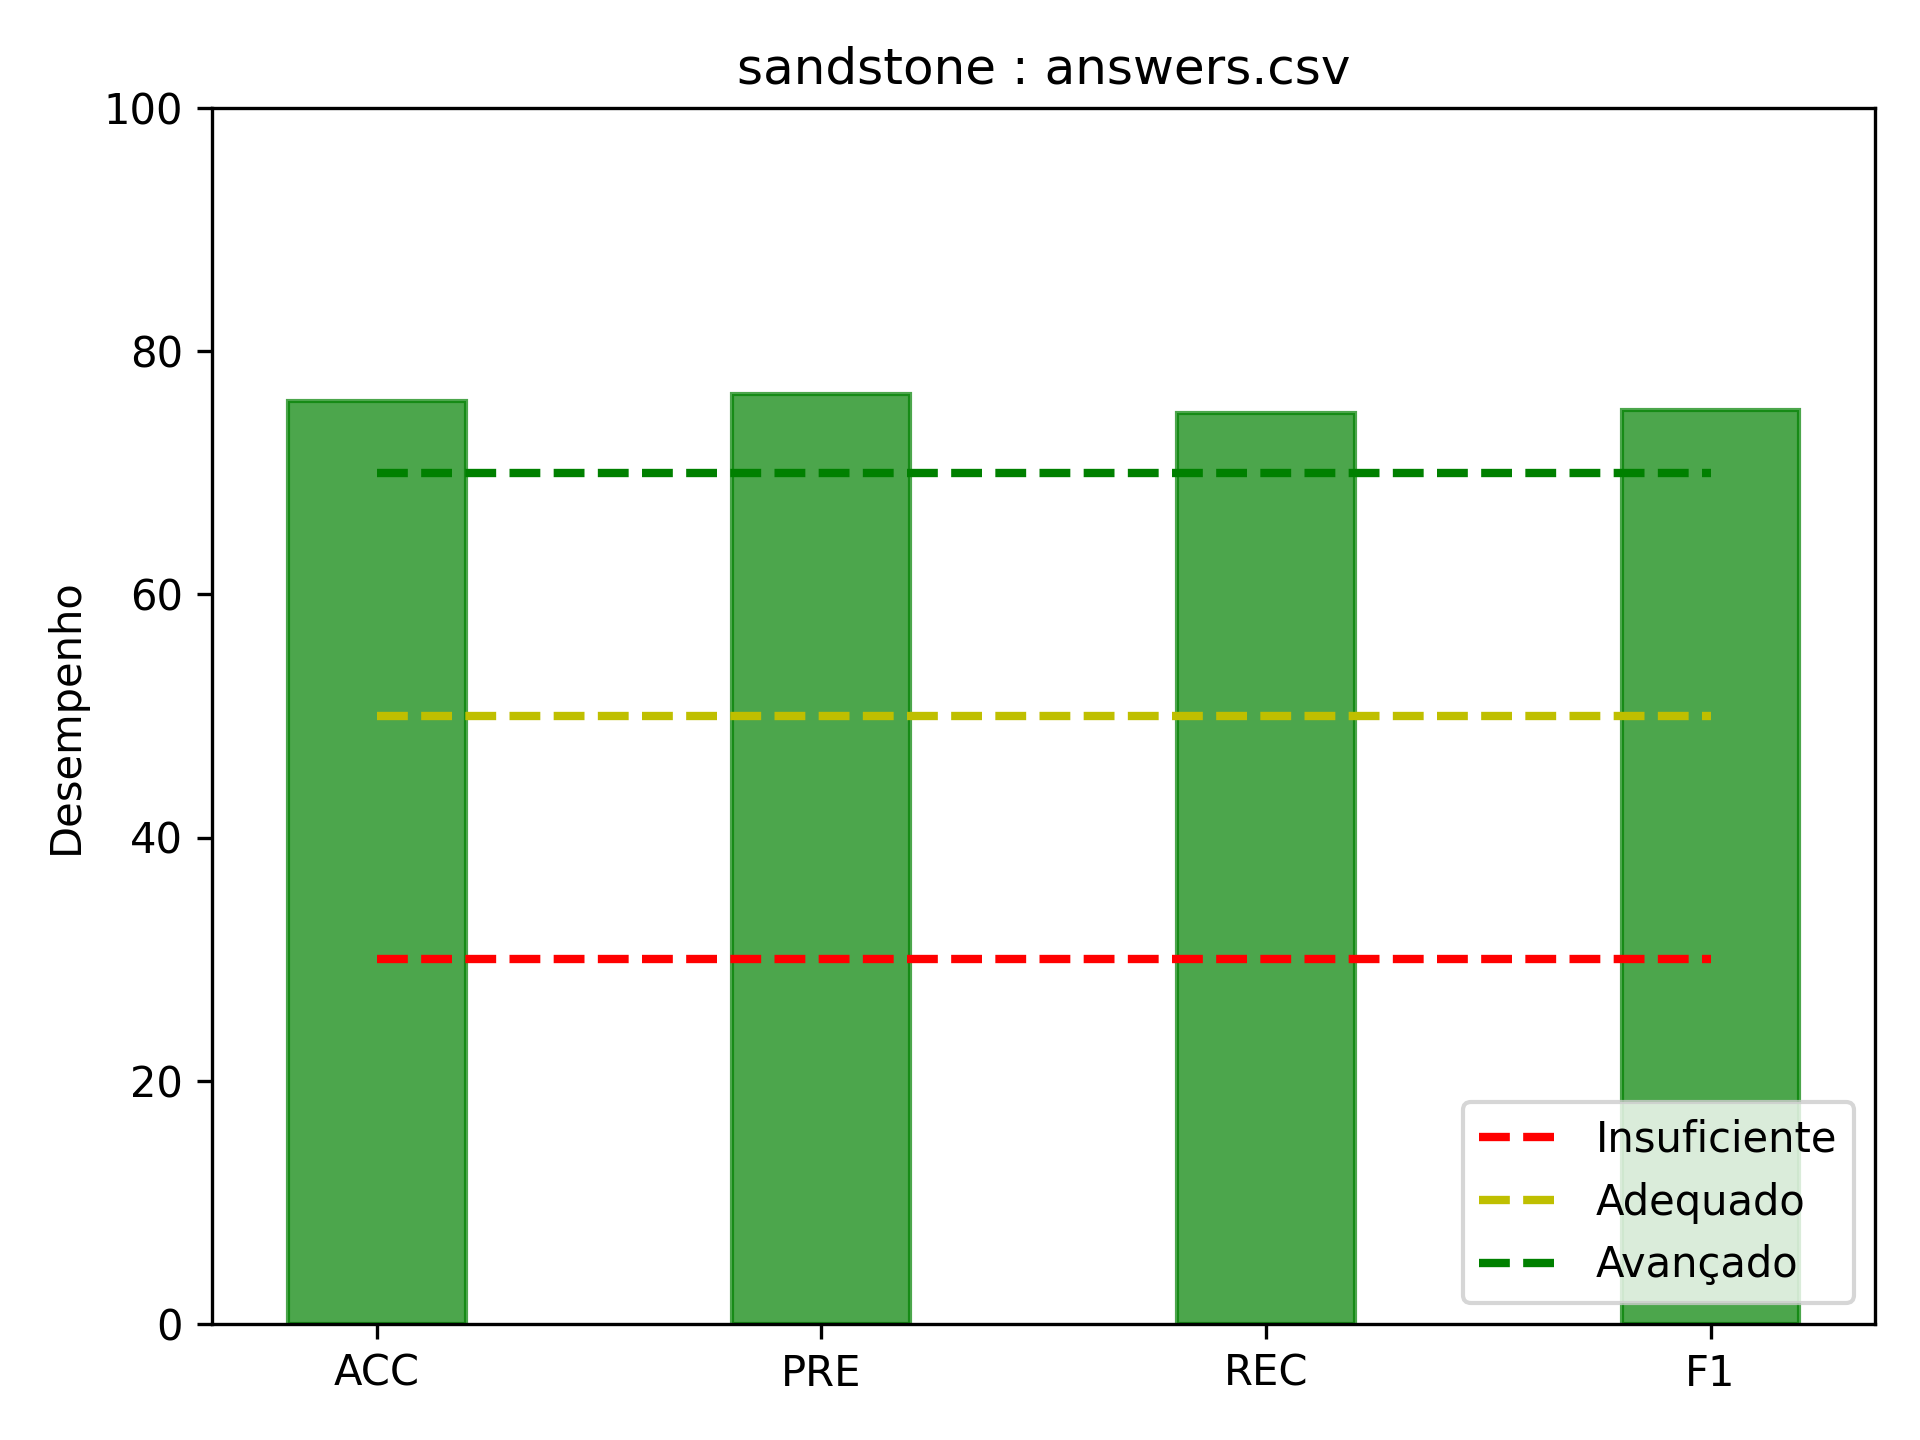
\includegraphics[width=\textwidth]{figuras/exemplo/sandstone-evalSVM.png}
 \caption{SVM}
\end{subfigure}
\hfill
\begin{subfigure}{0.4\textwidth}
 \centering
 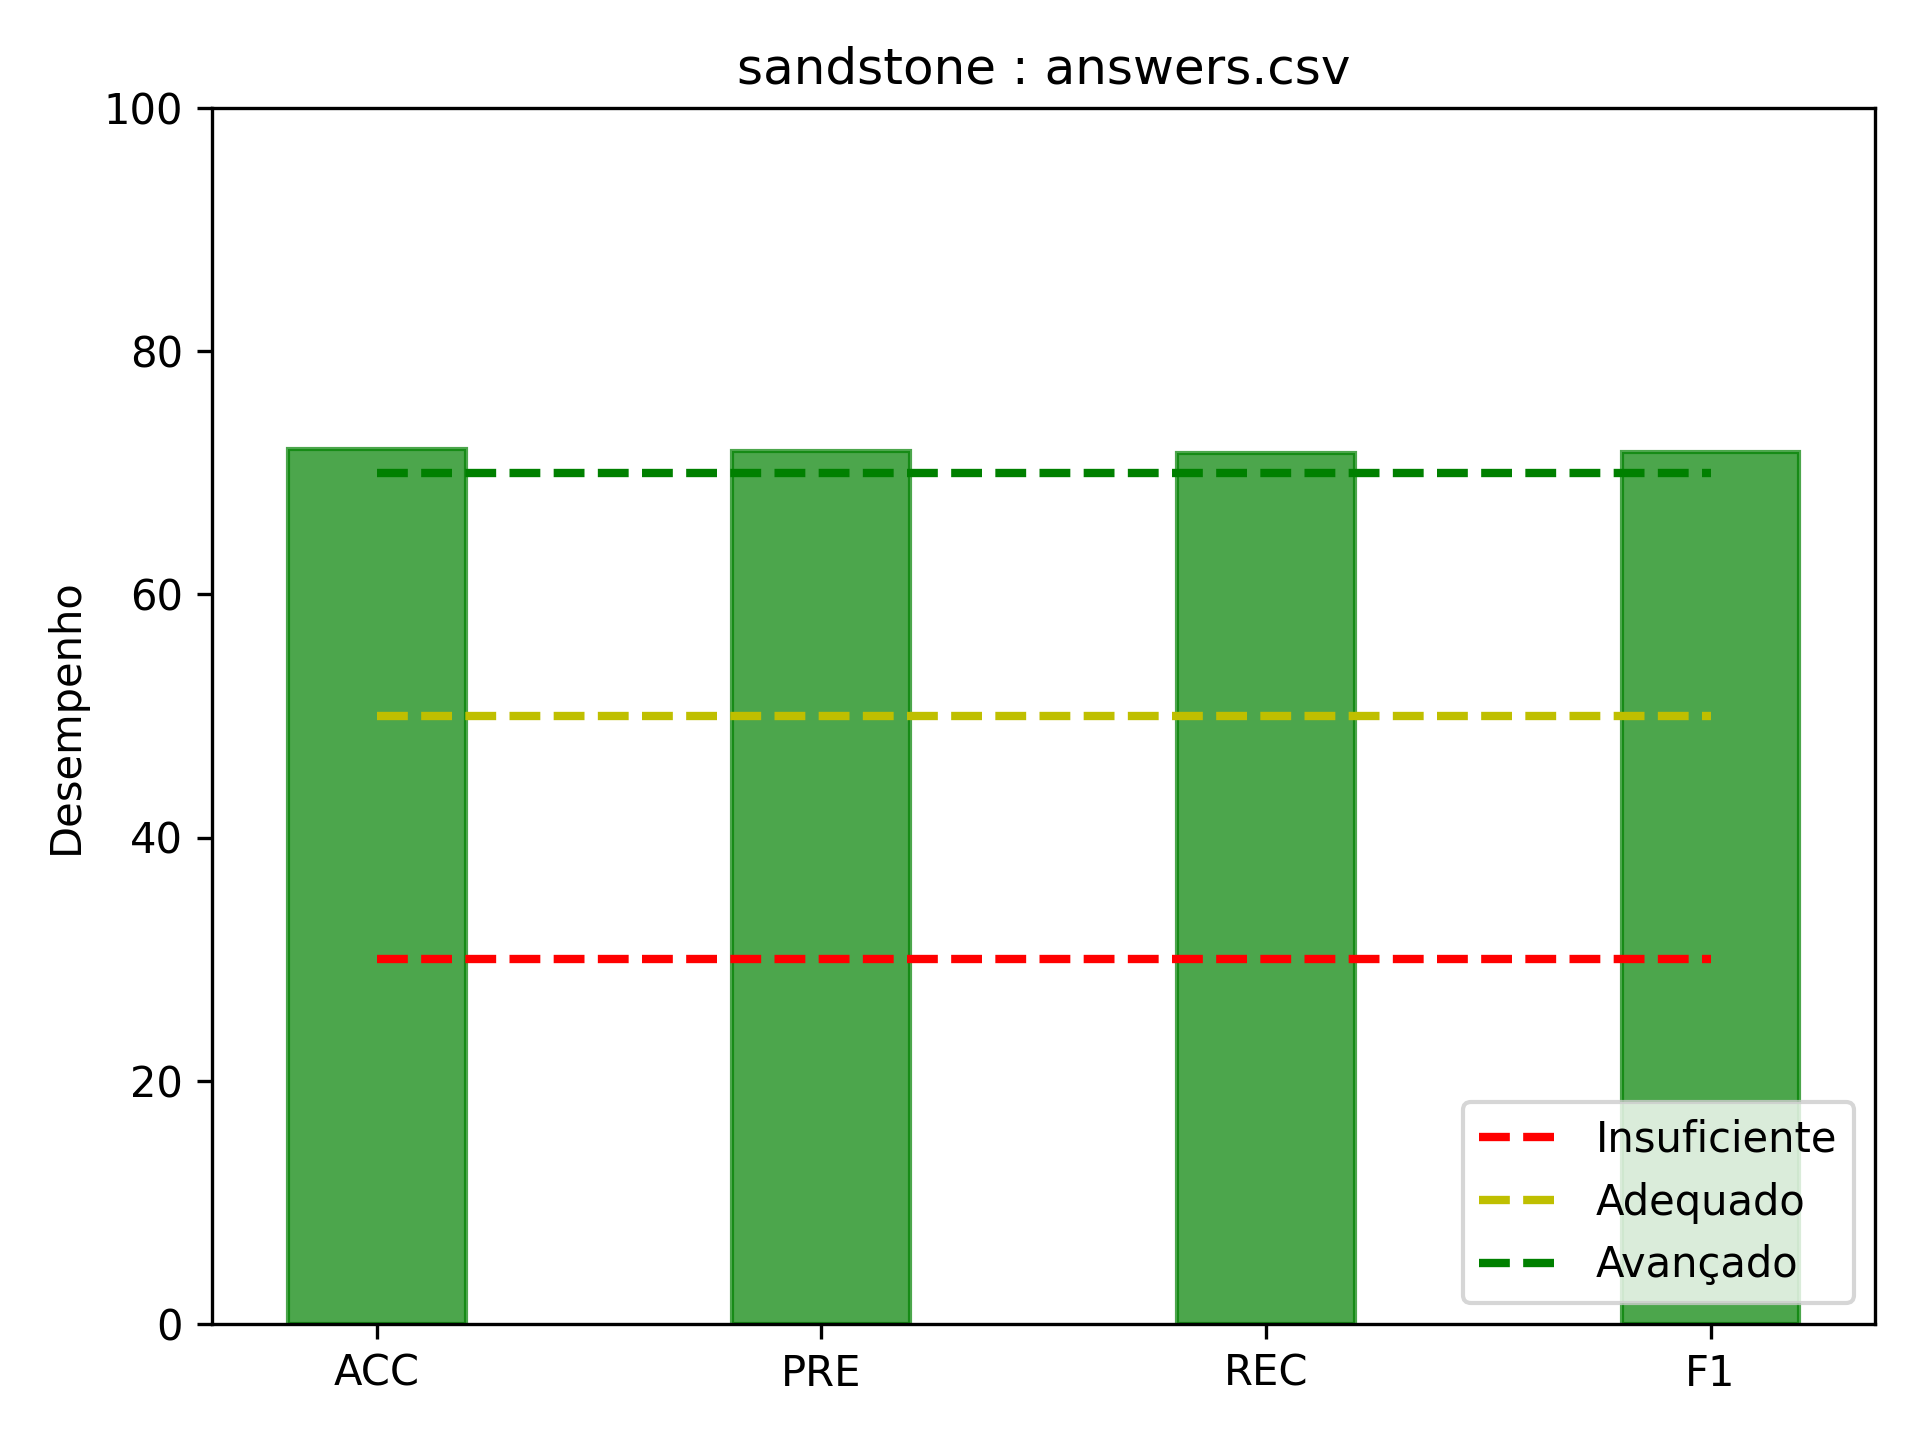
\includegraphics[width=\textwidth]{figuras/exemplo/sandstone-evalKNN.png}
 \caption{KNN}
\end{subfigure}
\hfill
\begin{subfigure}{0.4\textwidth}
 \centering
 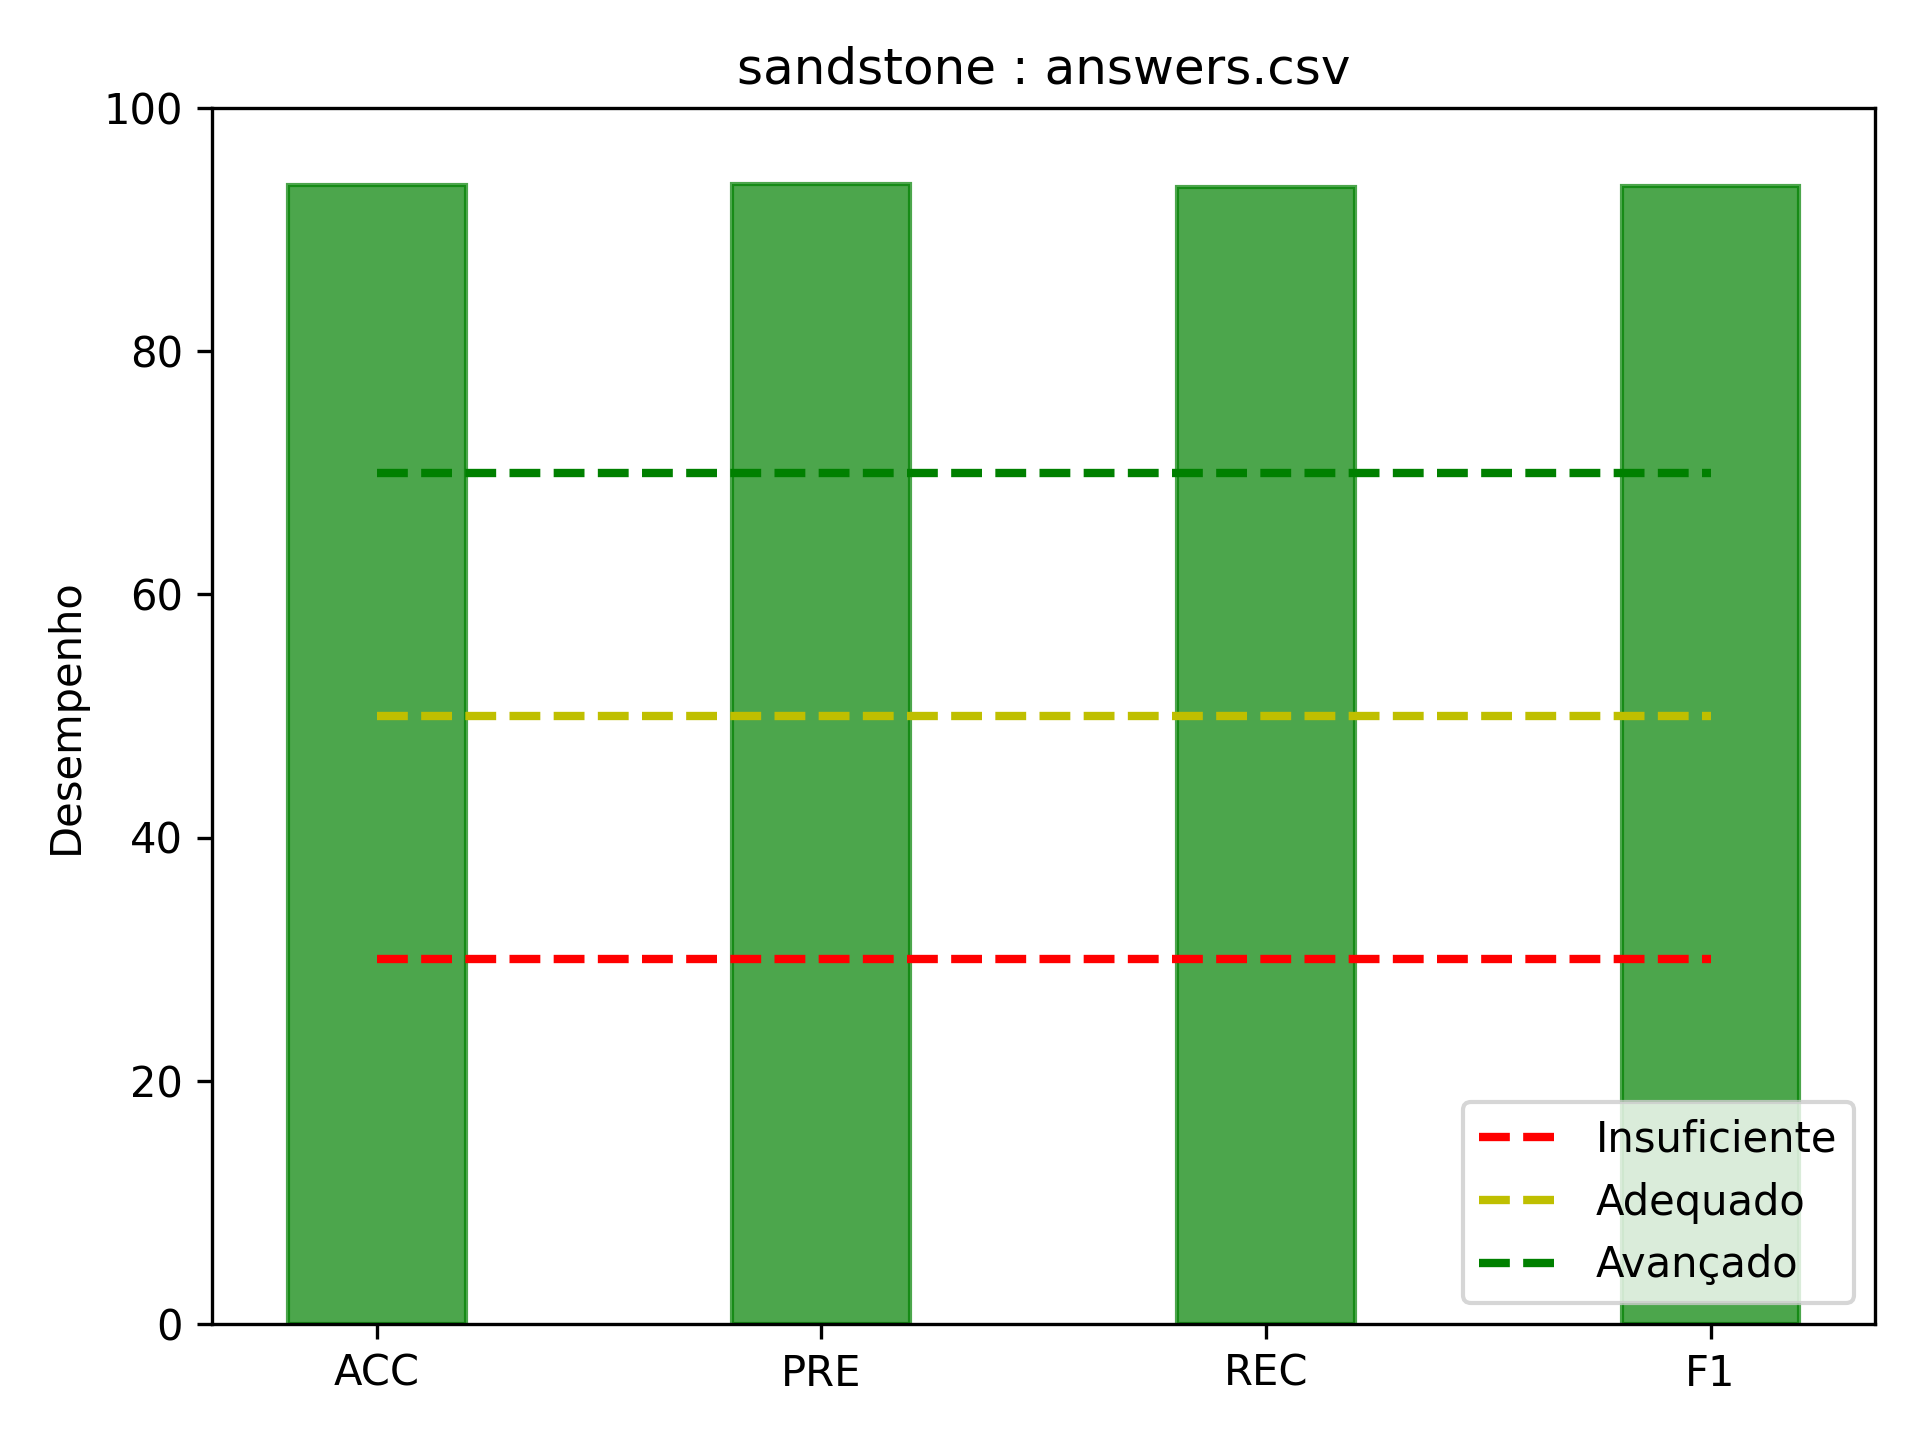
\includegraphics[width=\textwidth]{figuras/exemplo/sandstone-evalDTR.png}
 \caption{DTR}
\end{subfigure}
\hfill
\begin{subfigure}{0.4\textwidth}
 \centering
 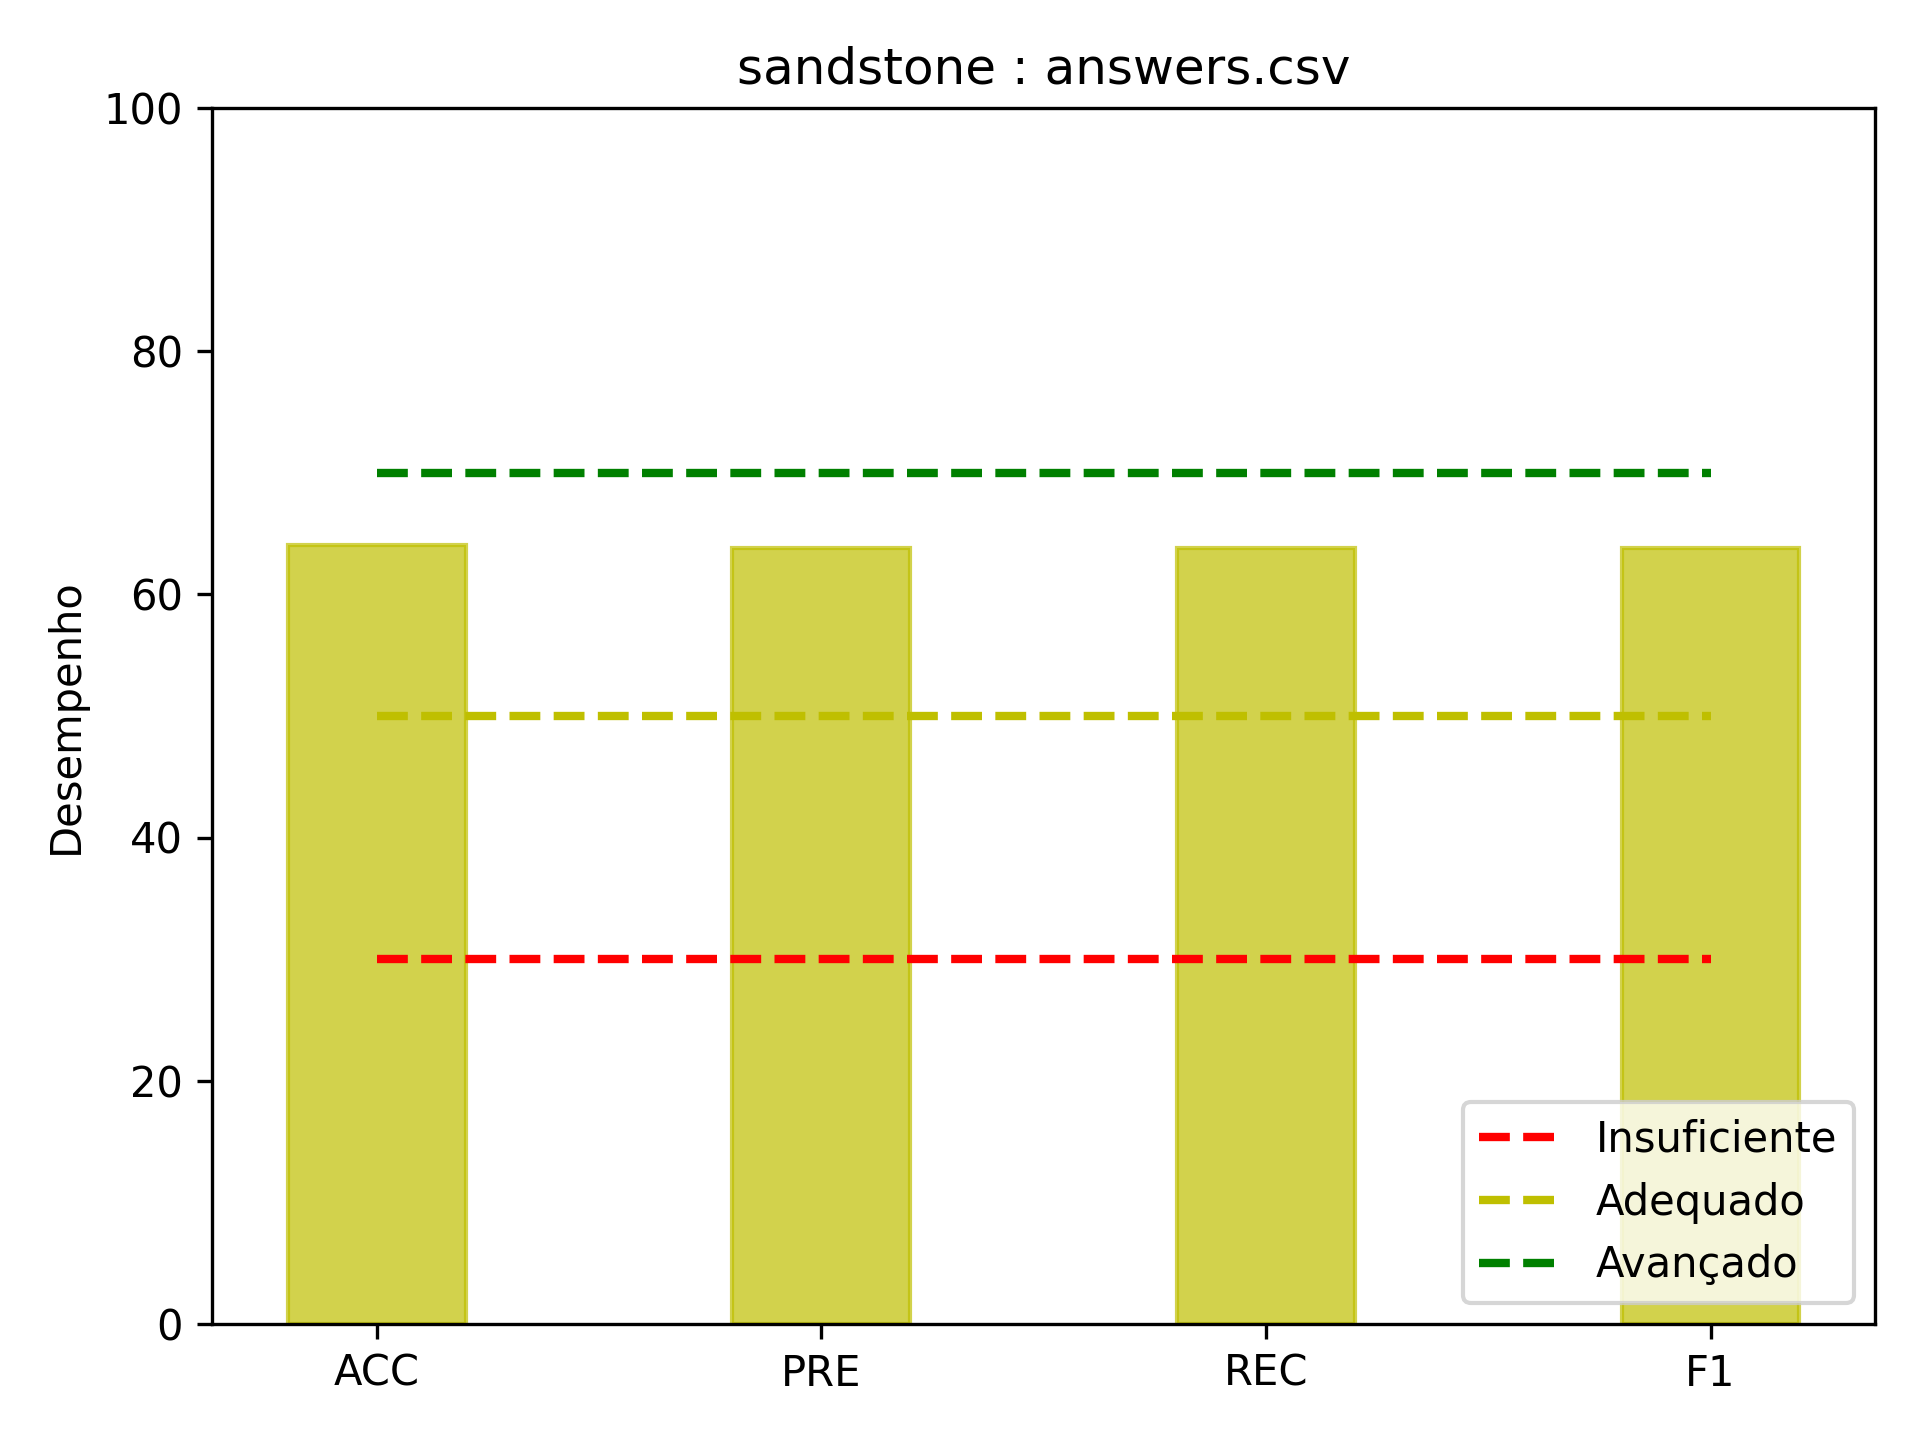
\includegraphics[width=\textwidth]{figuras/exemplo/sandstone-evalWSD.png}
 \caption{WSD}
\end{subfigure}
\hfill
\begin{subfigure}{0.4\textwidth}
 \centering
 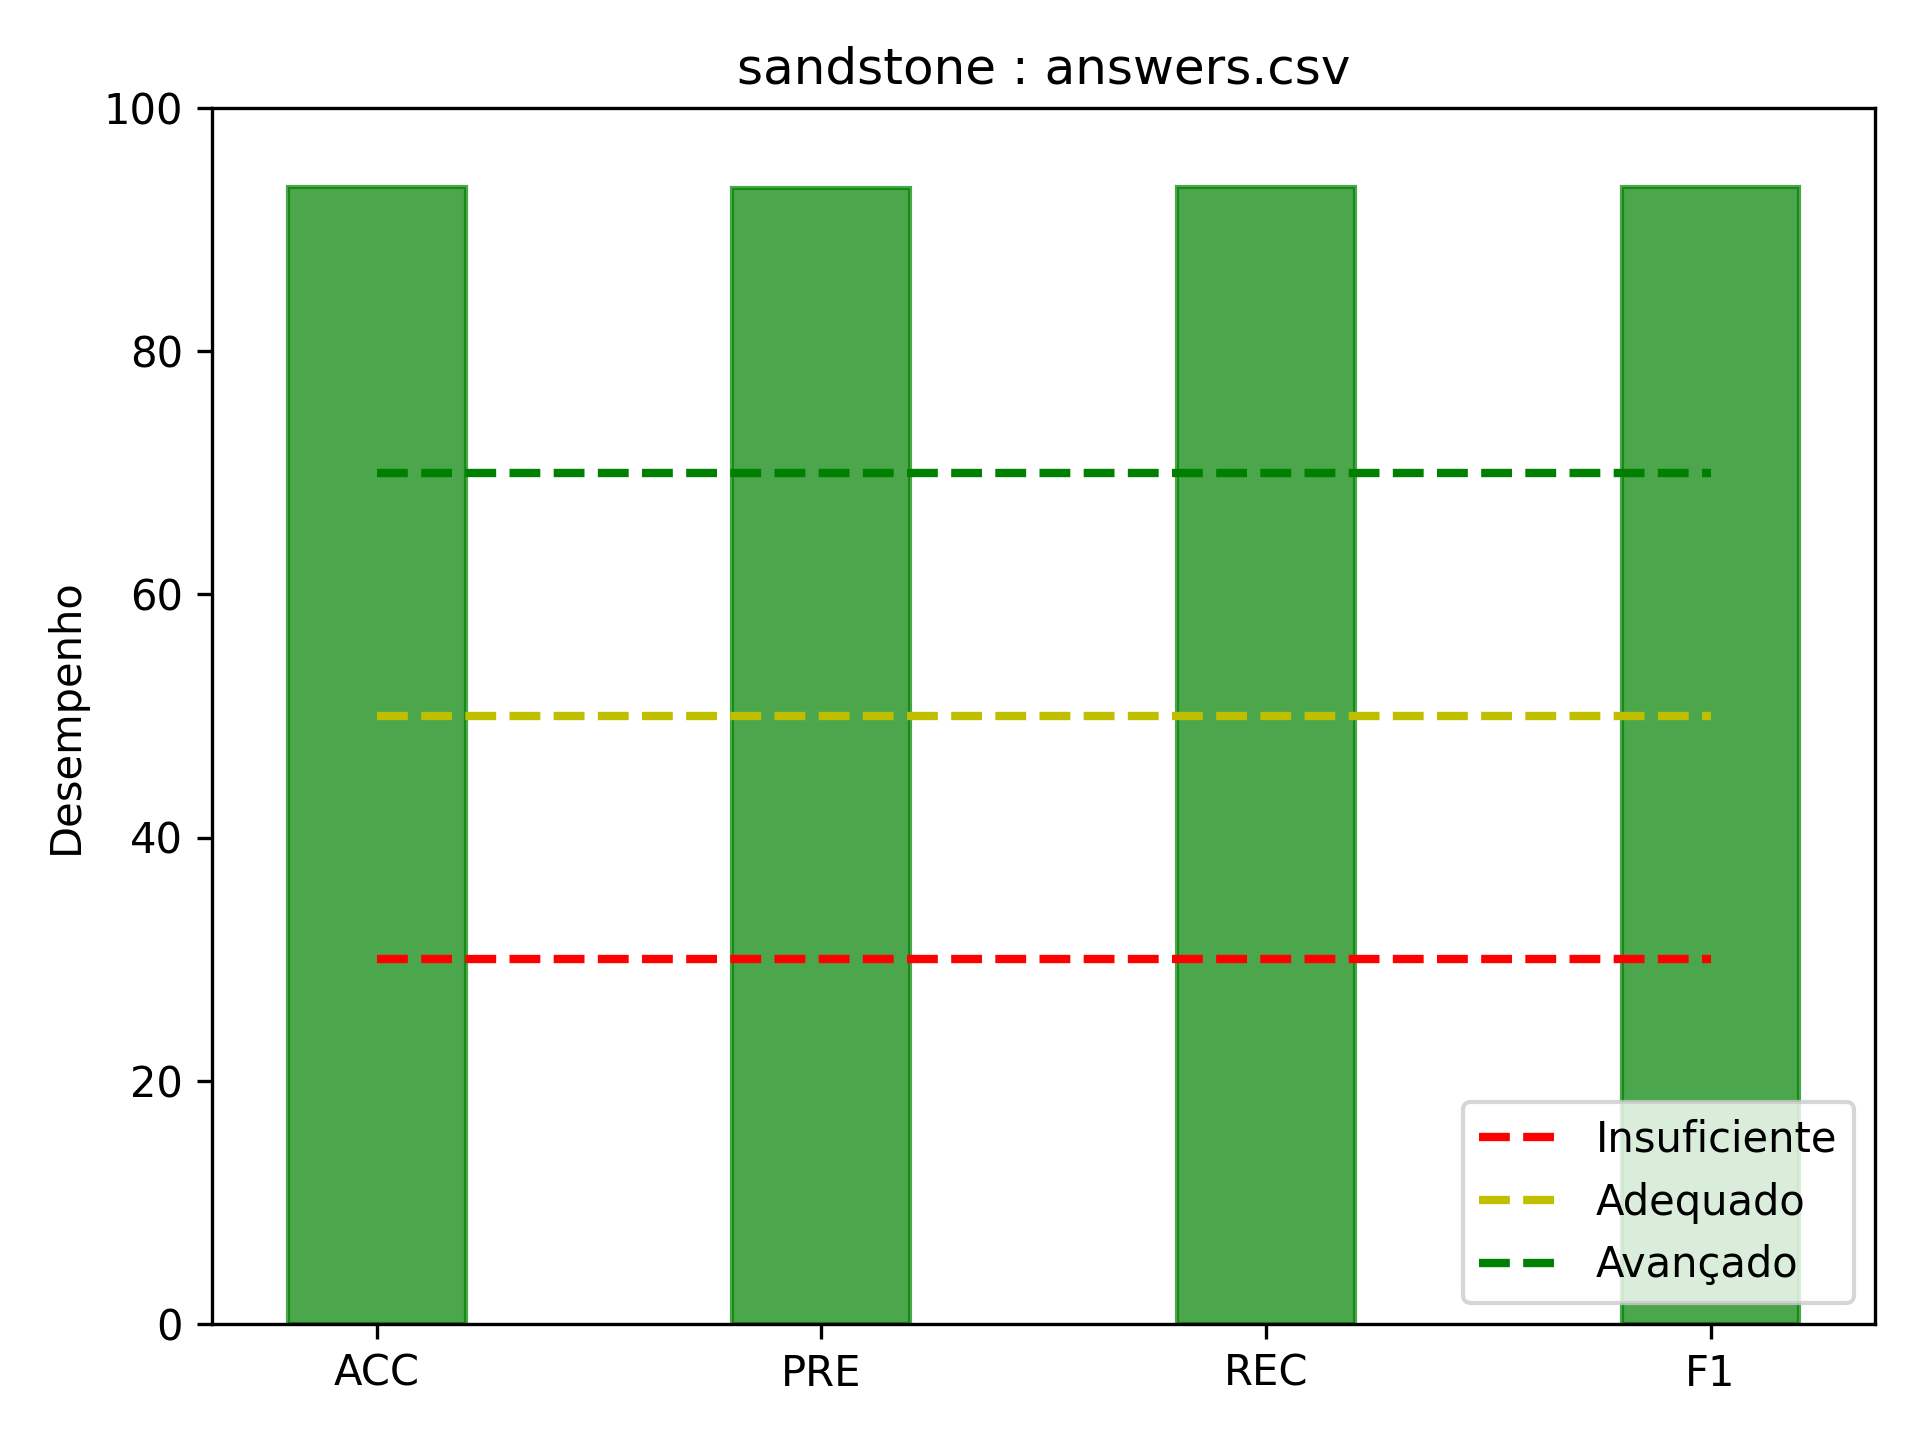
\includegraphics[width=\textwidth]{figuras/exemplo/sandstone-evalGBC.png}
 \caption{GBC}
\end{subfigure}
\hfill
\begin{subfigure}{0.4\textwidth}
 \centering
 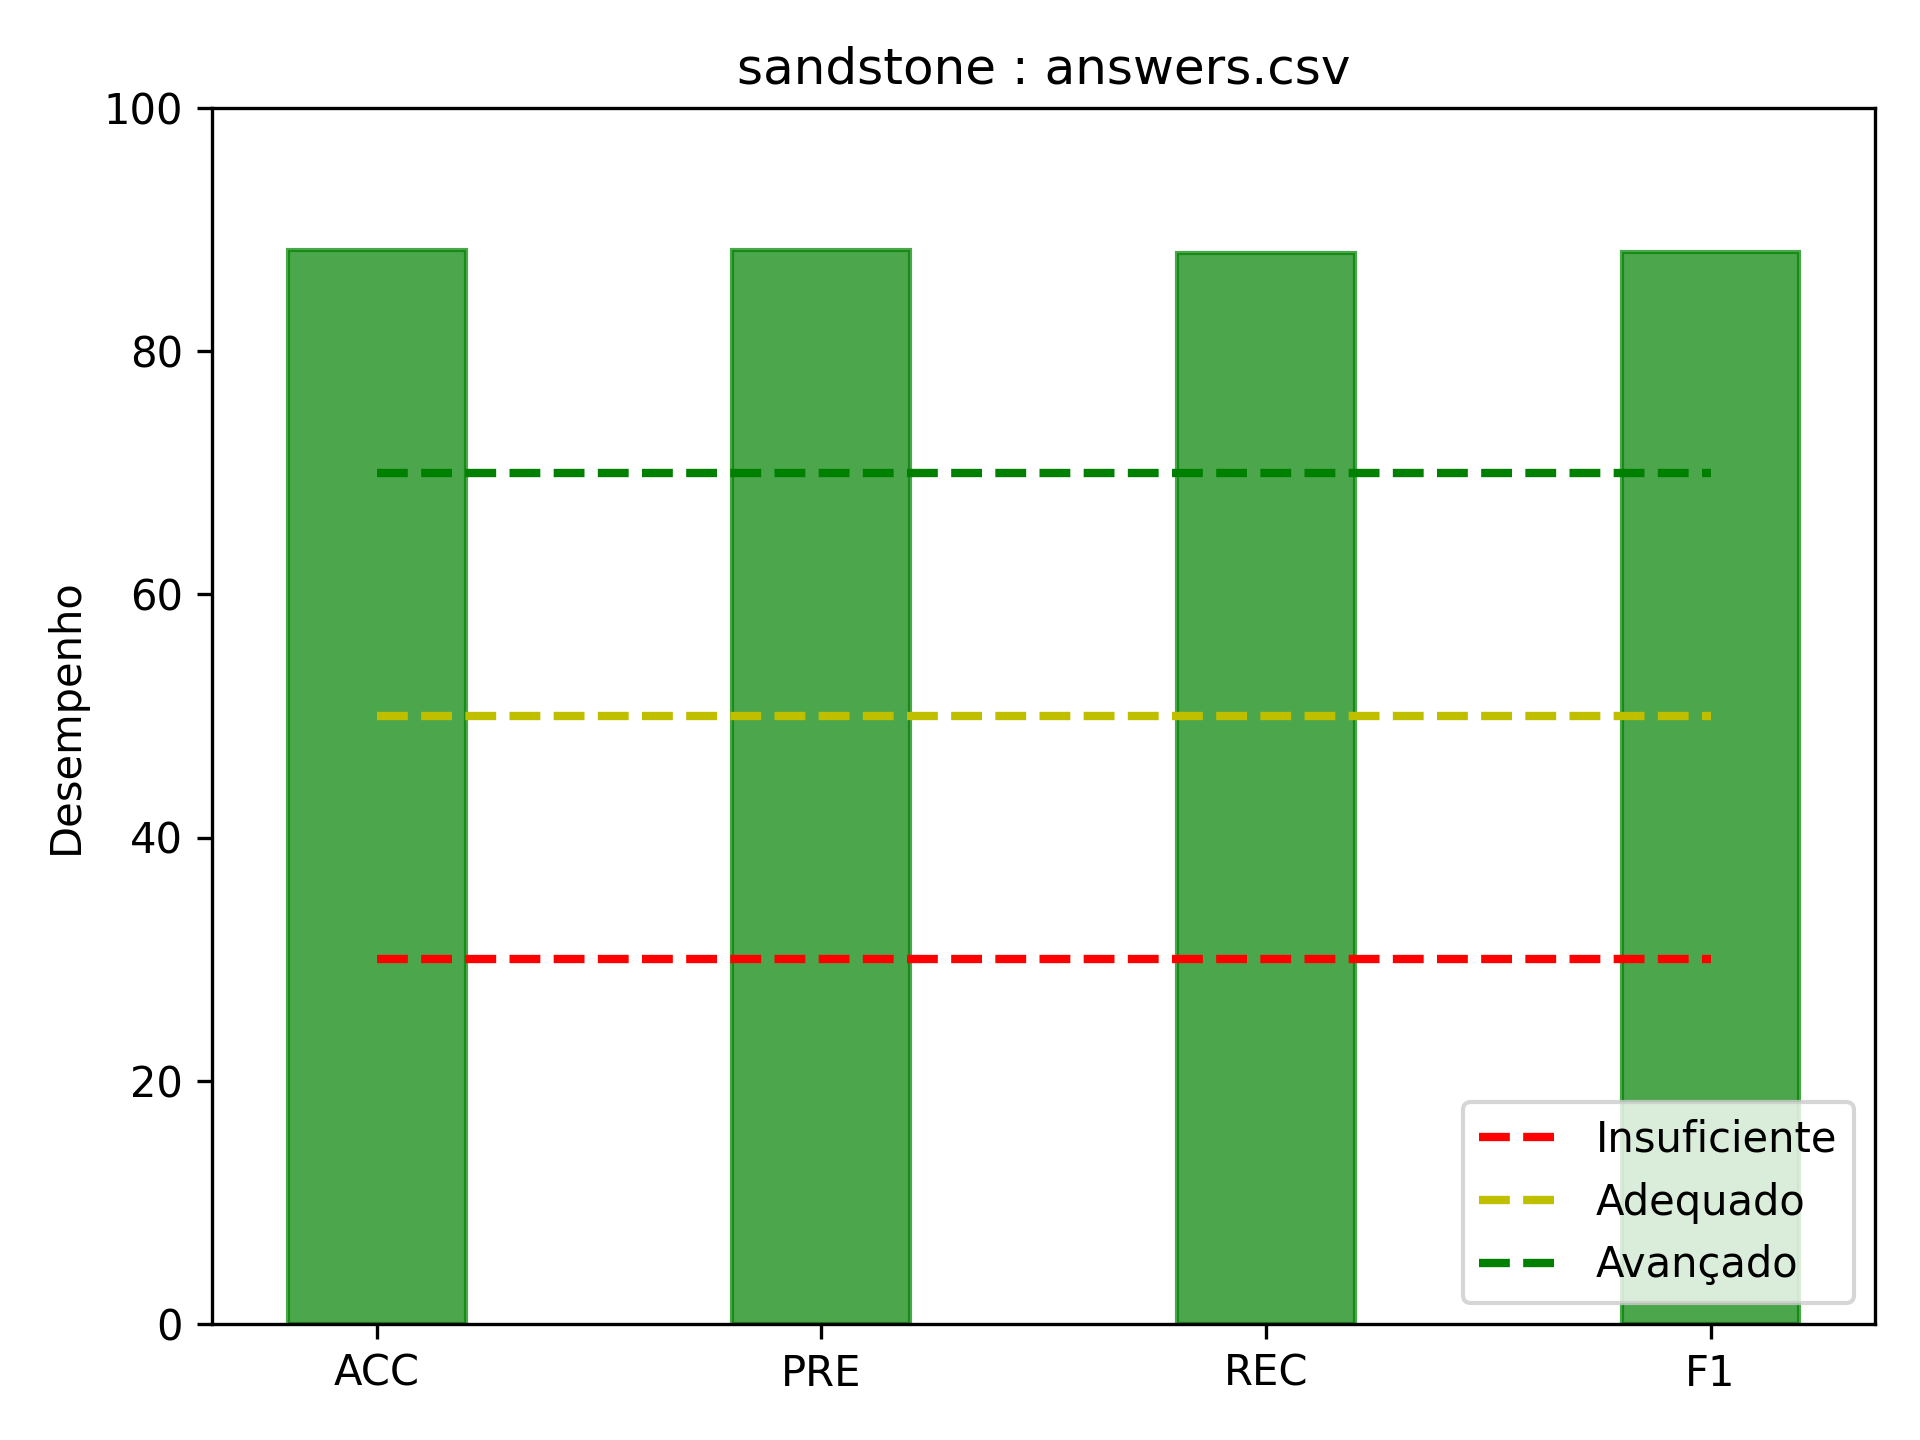
\includegraphics[width=\textwidth]{figuras/exemplo/sandstone-evalRDF.png}
 \caption{RDF}
\end{subfigure}
\caption{Resultados de todos os 6 algoritmos de classificação para a atividade exemplo.}
\label{fig-exemplo-clf}
\end{figure}

\begin{figure}[!h]
\begin{subfigure}{0.4\textwidth}
 \centering
 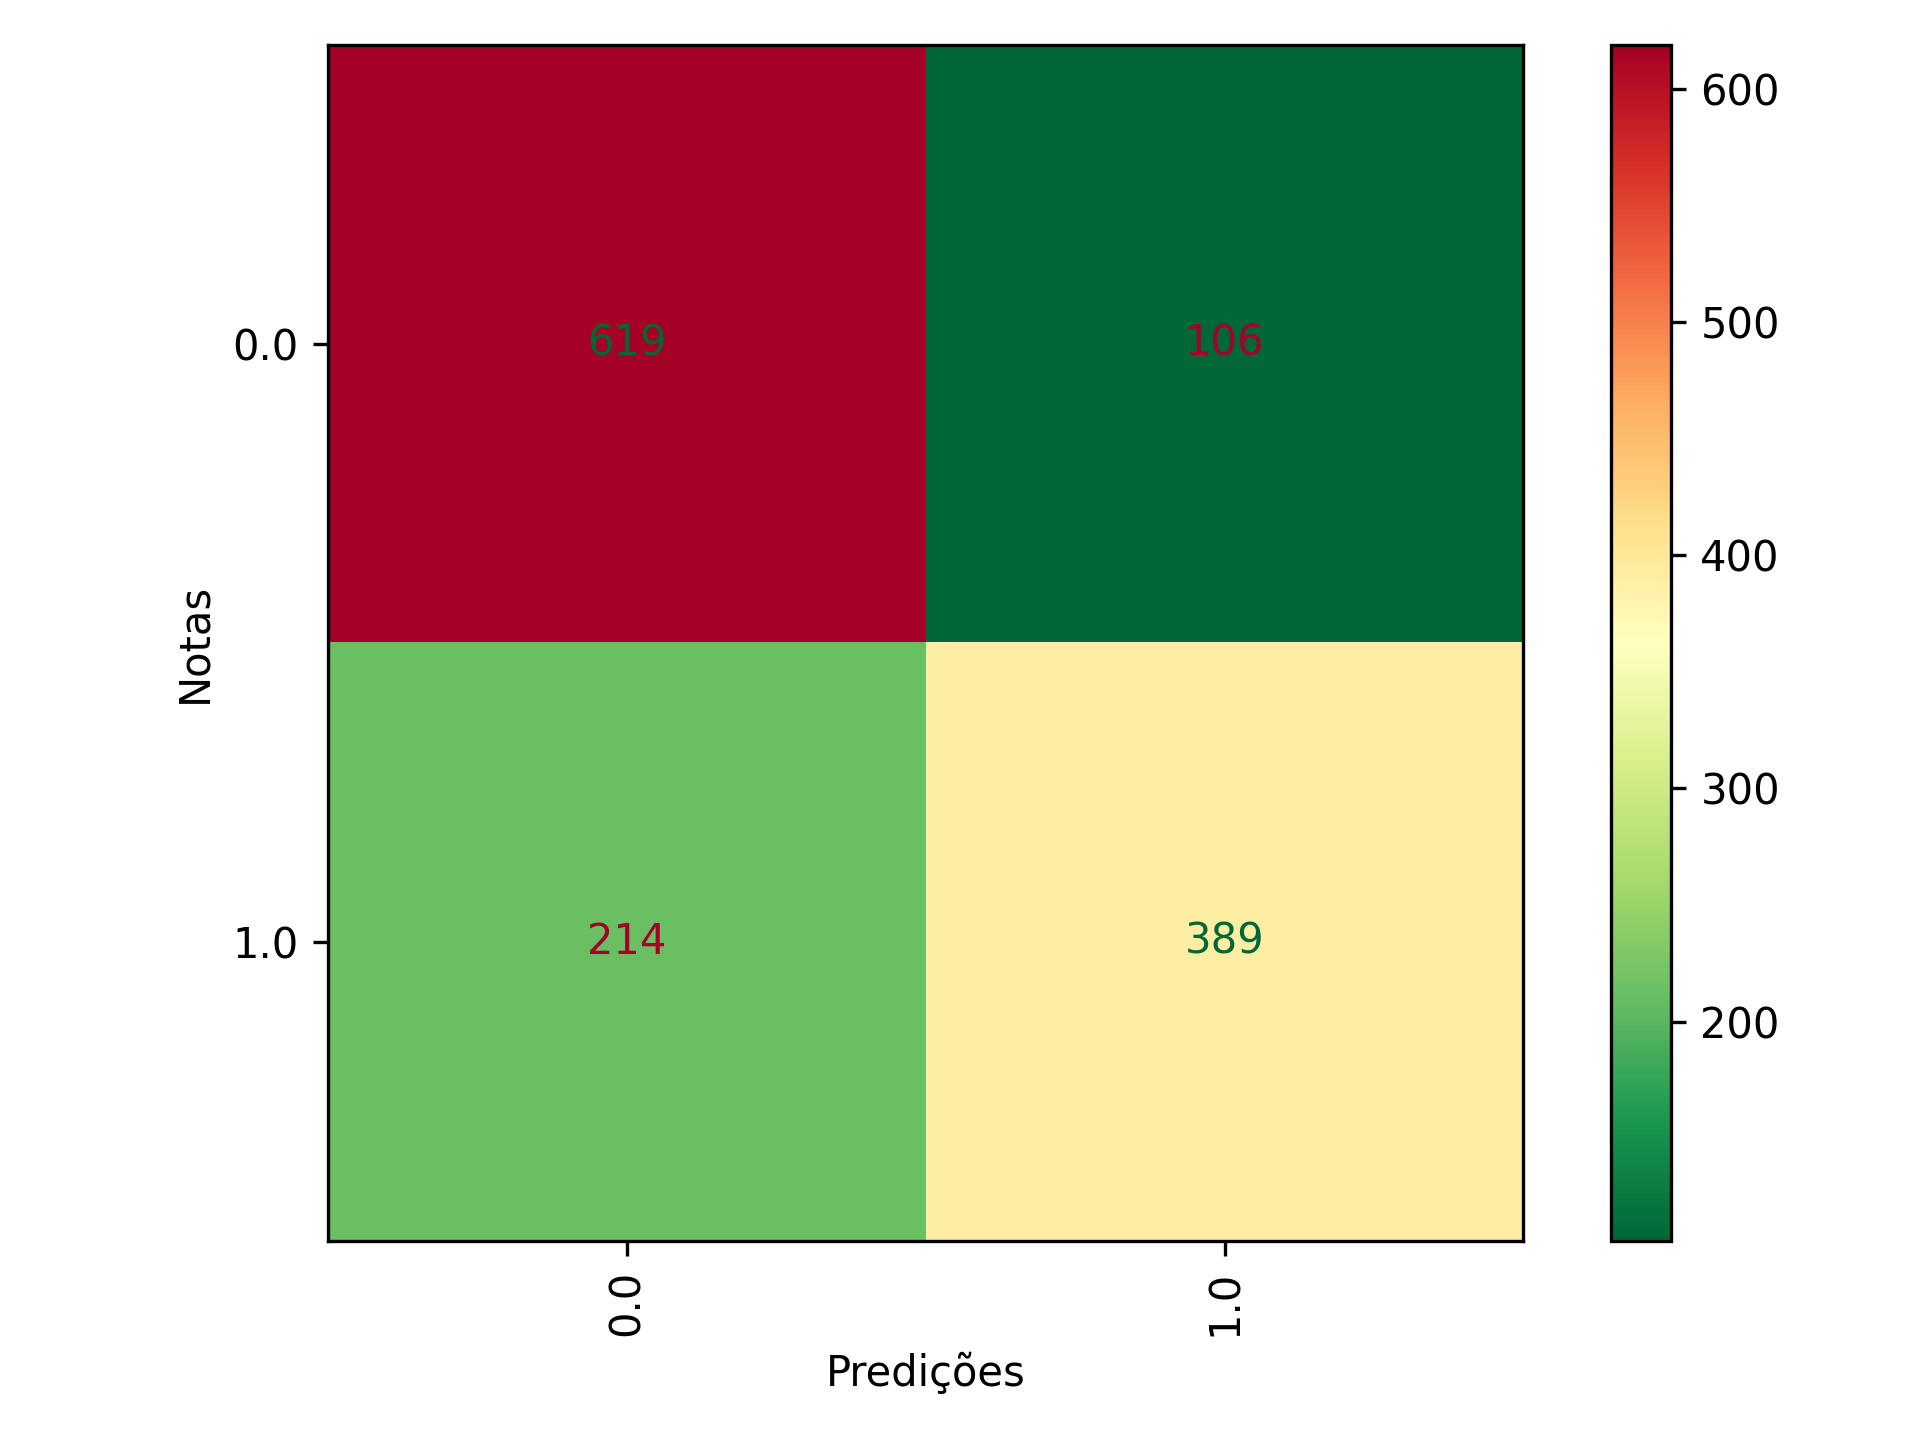
\includegraphics[width=\textwidth]{figuras/exemplo/sandstone-cmSVM.png}
 \caption{SVM}
\end{subfigure}
\hfill
\begin{subfigure}{0.4\textwidth}
 \centering
 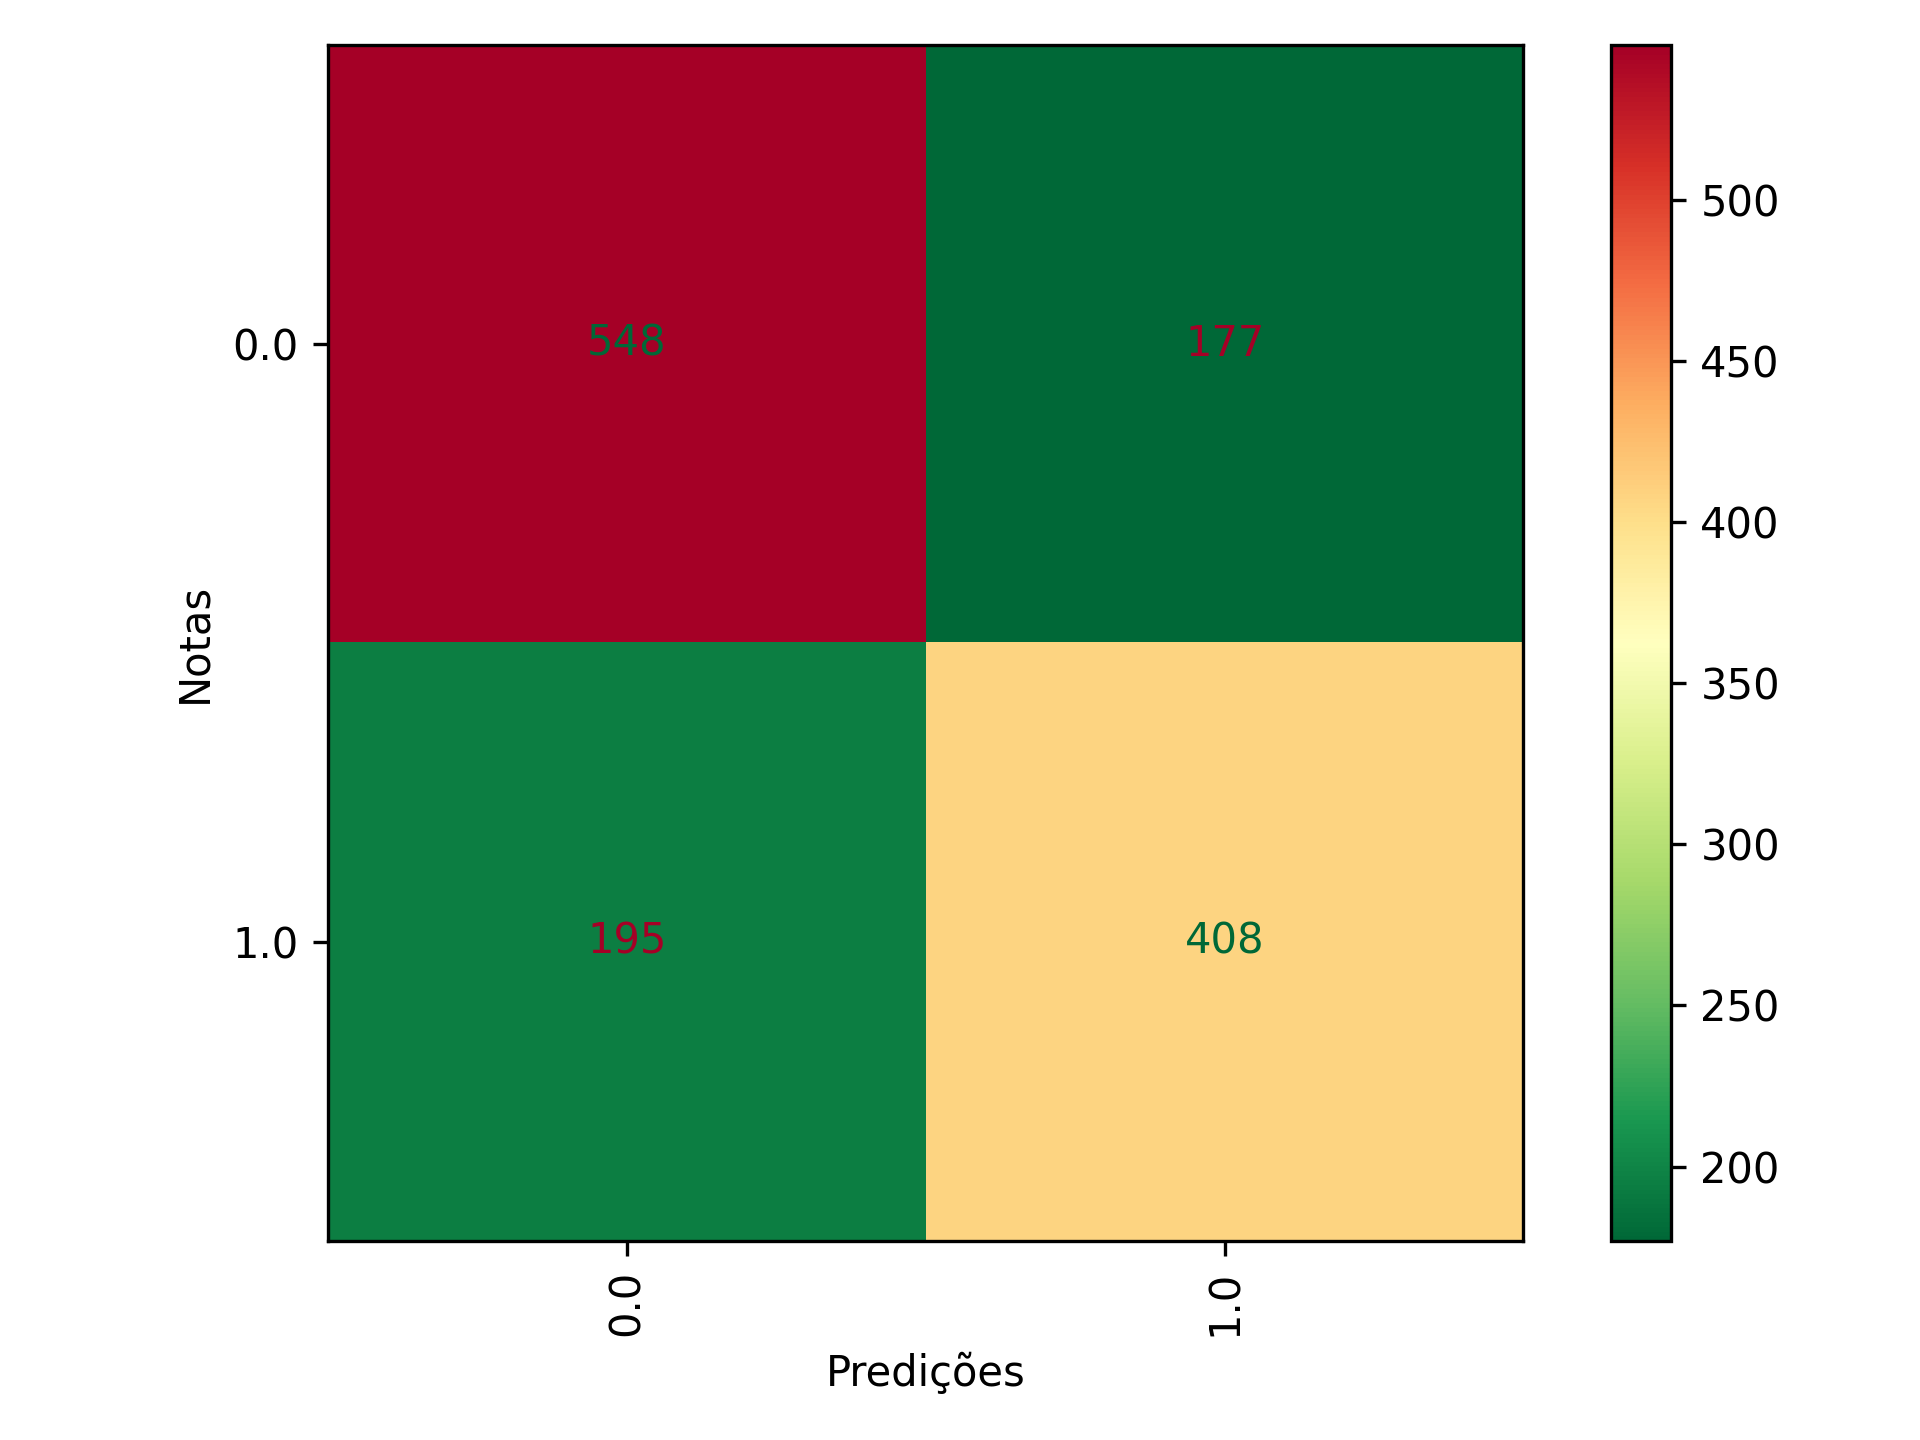
\includegraphics[width=\textwidth]{figuras/exemplo/sandstone-cmKNN.png}
 \caption{KNN}
\end{subfigure}
\hfill
\begin{subfigure}{0.4\textwidth}
 \centering
 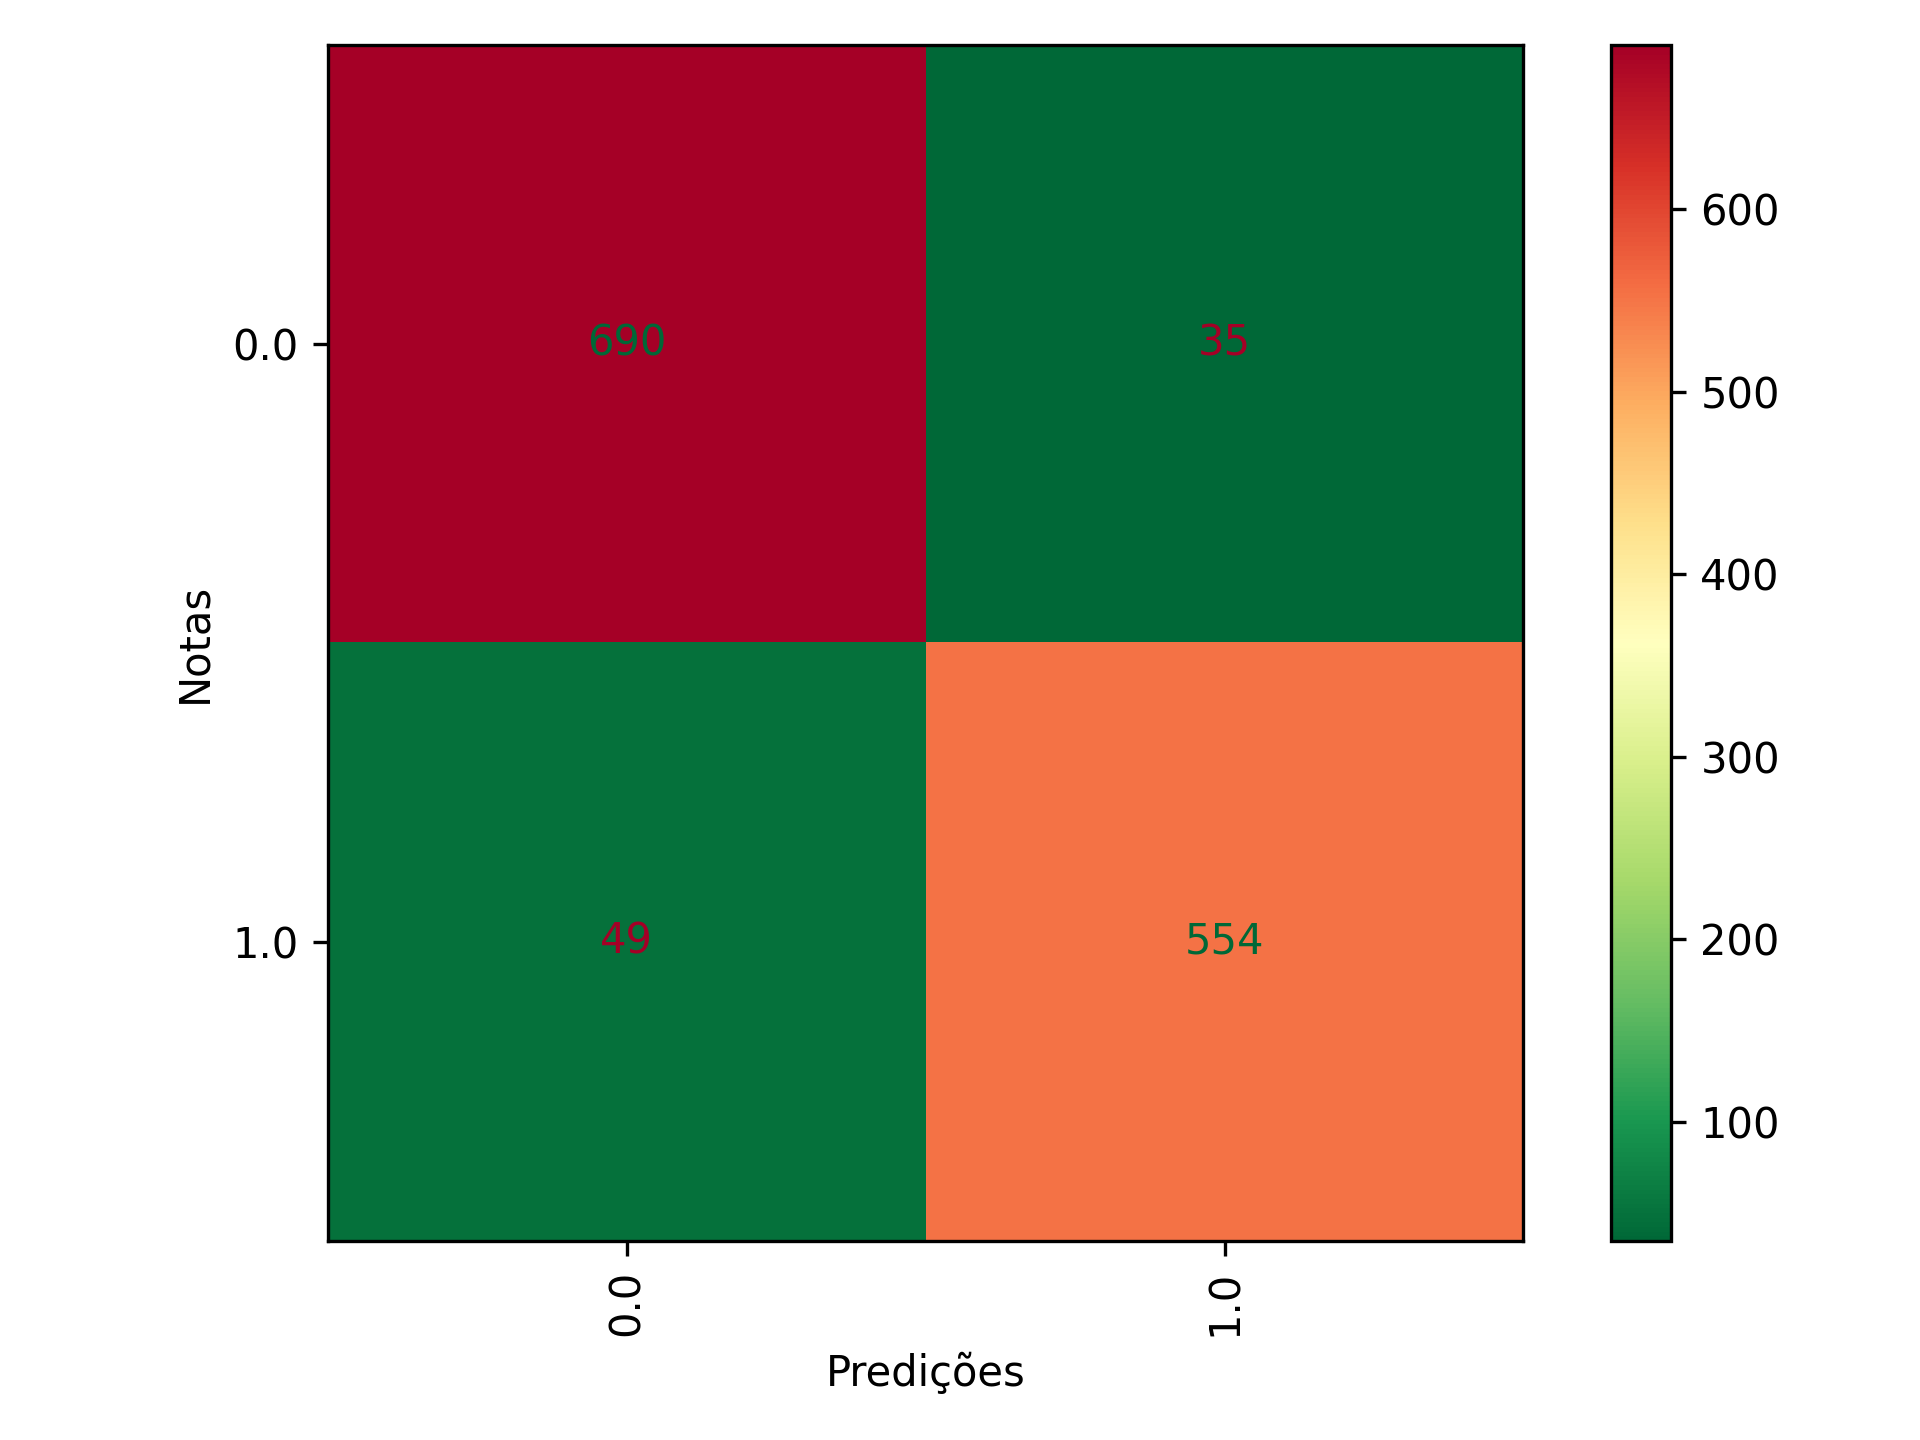
\includegraphics[width=\textwidth]{figuras/exemplo/sandstone-cmDTR.png}
 \caption{DTR}
\end{subfigure}
\hfill
\begin{subfigure}{0.4\textwidth}
 \centering
 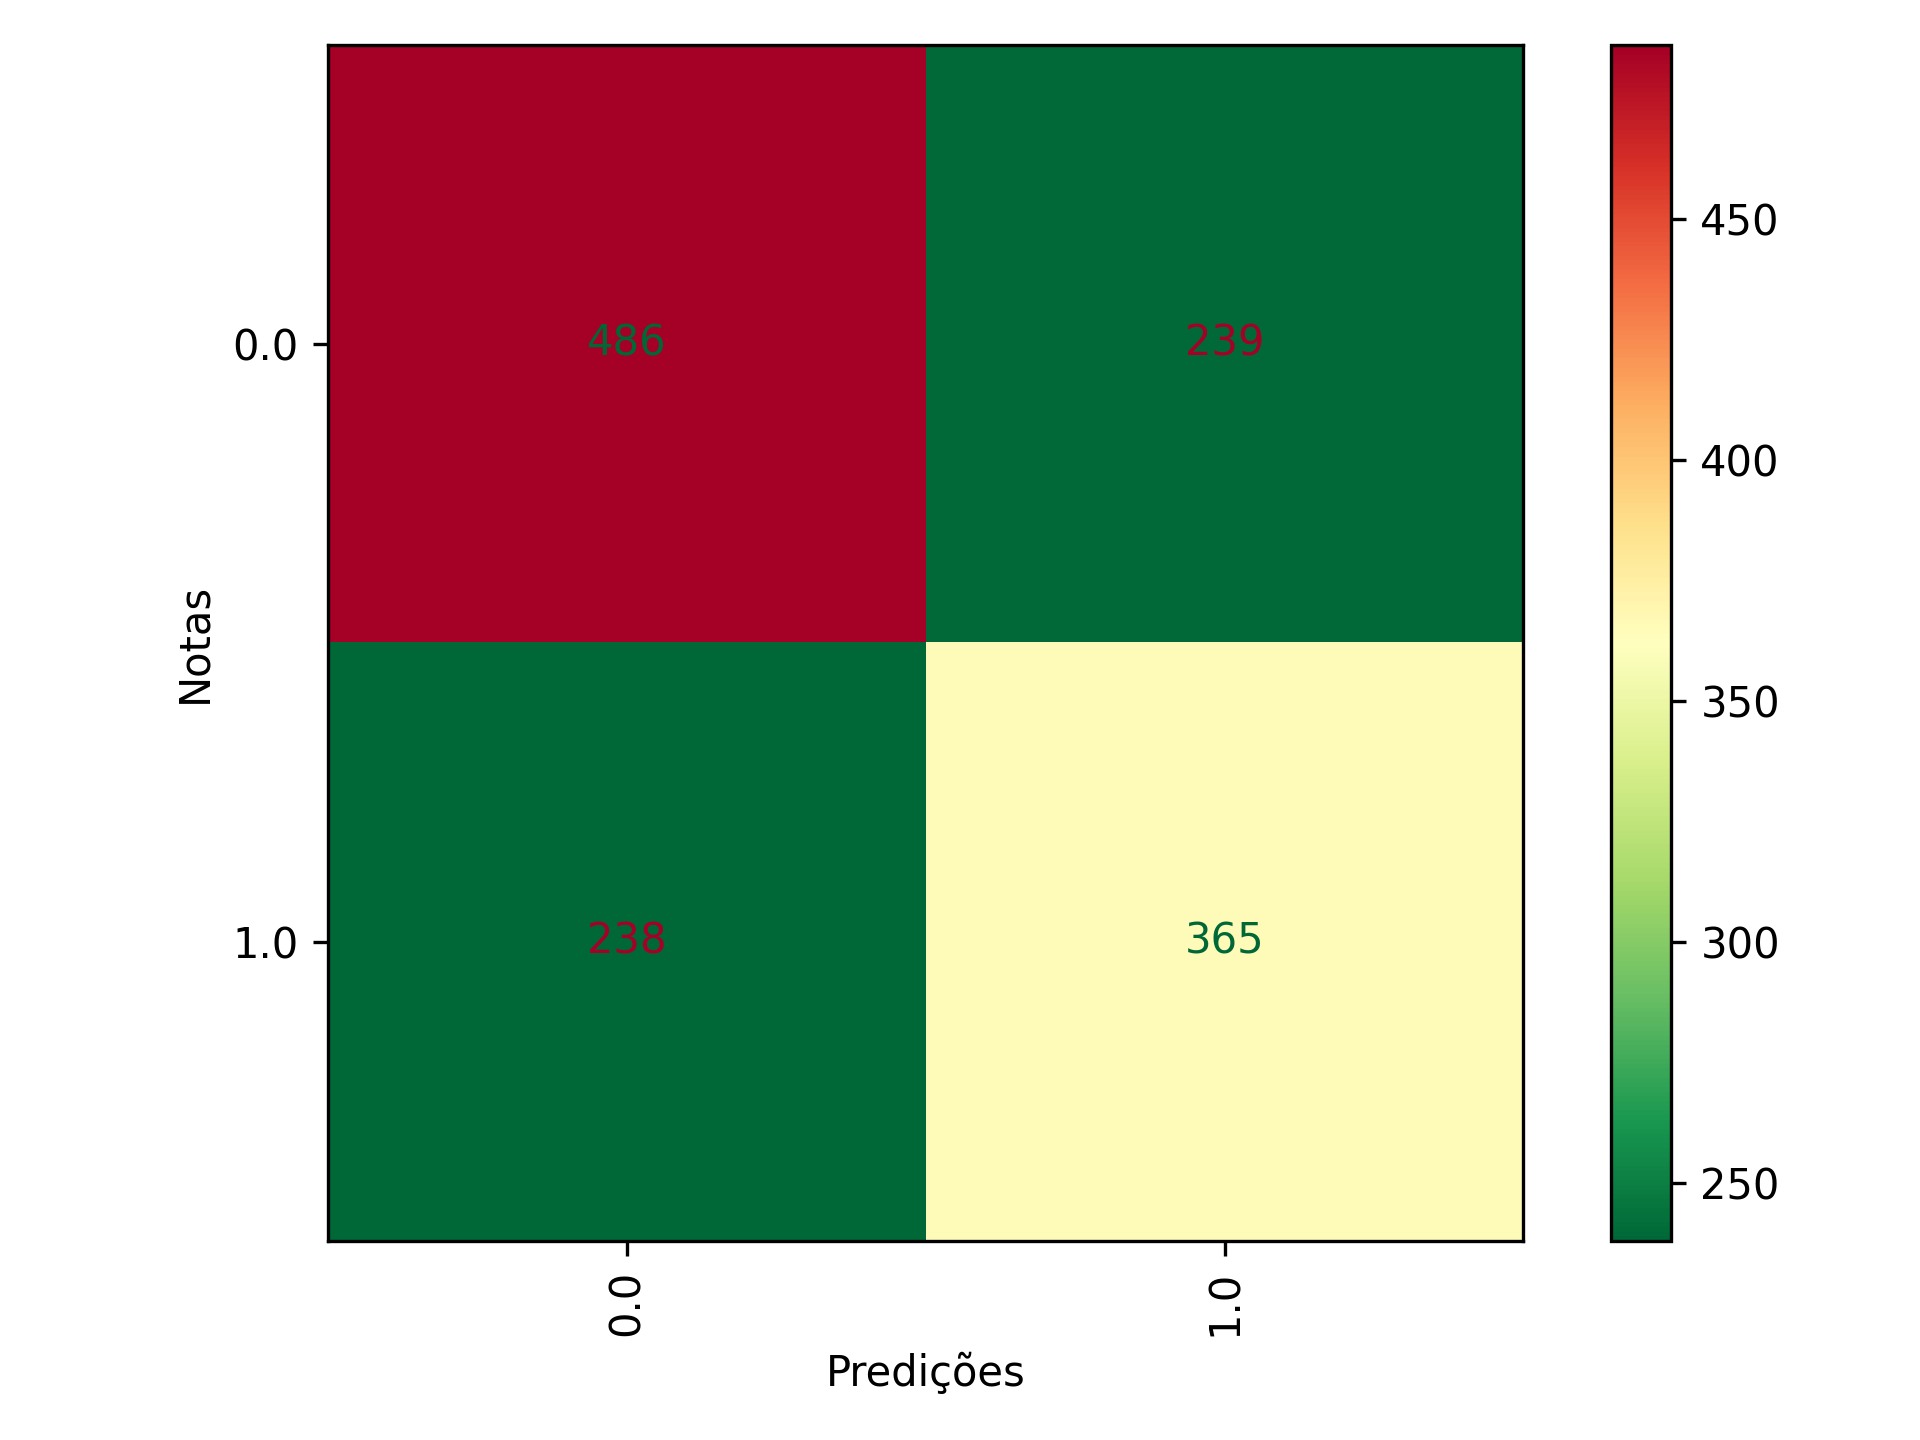
\includegraphics[width=\textwidth]{figuras/exemplo/sandstone-cmWSD.png}
 \caption{WSD}
\end{subfigure}
\hfill
\begin{subfigure}{0.4\textwidth}
 \centering
 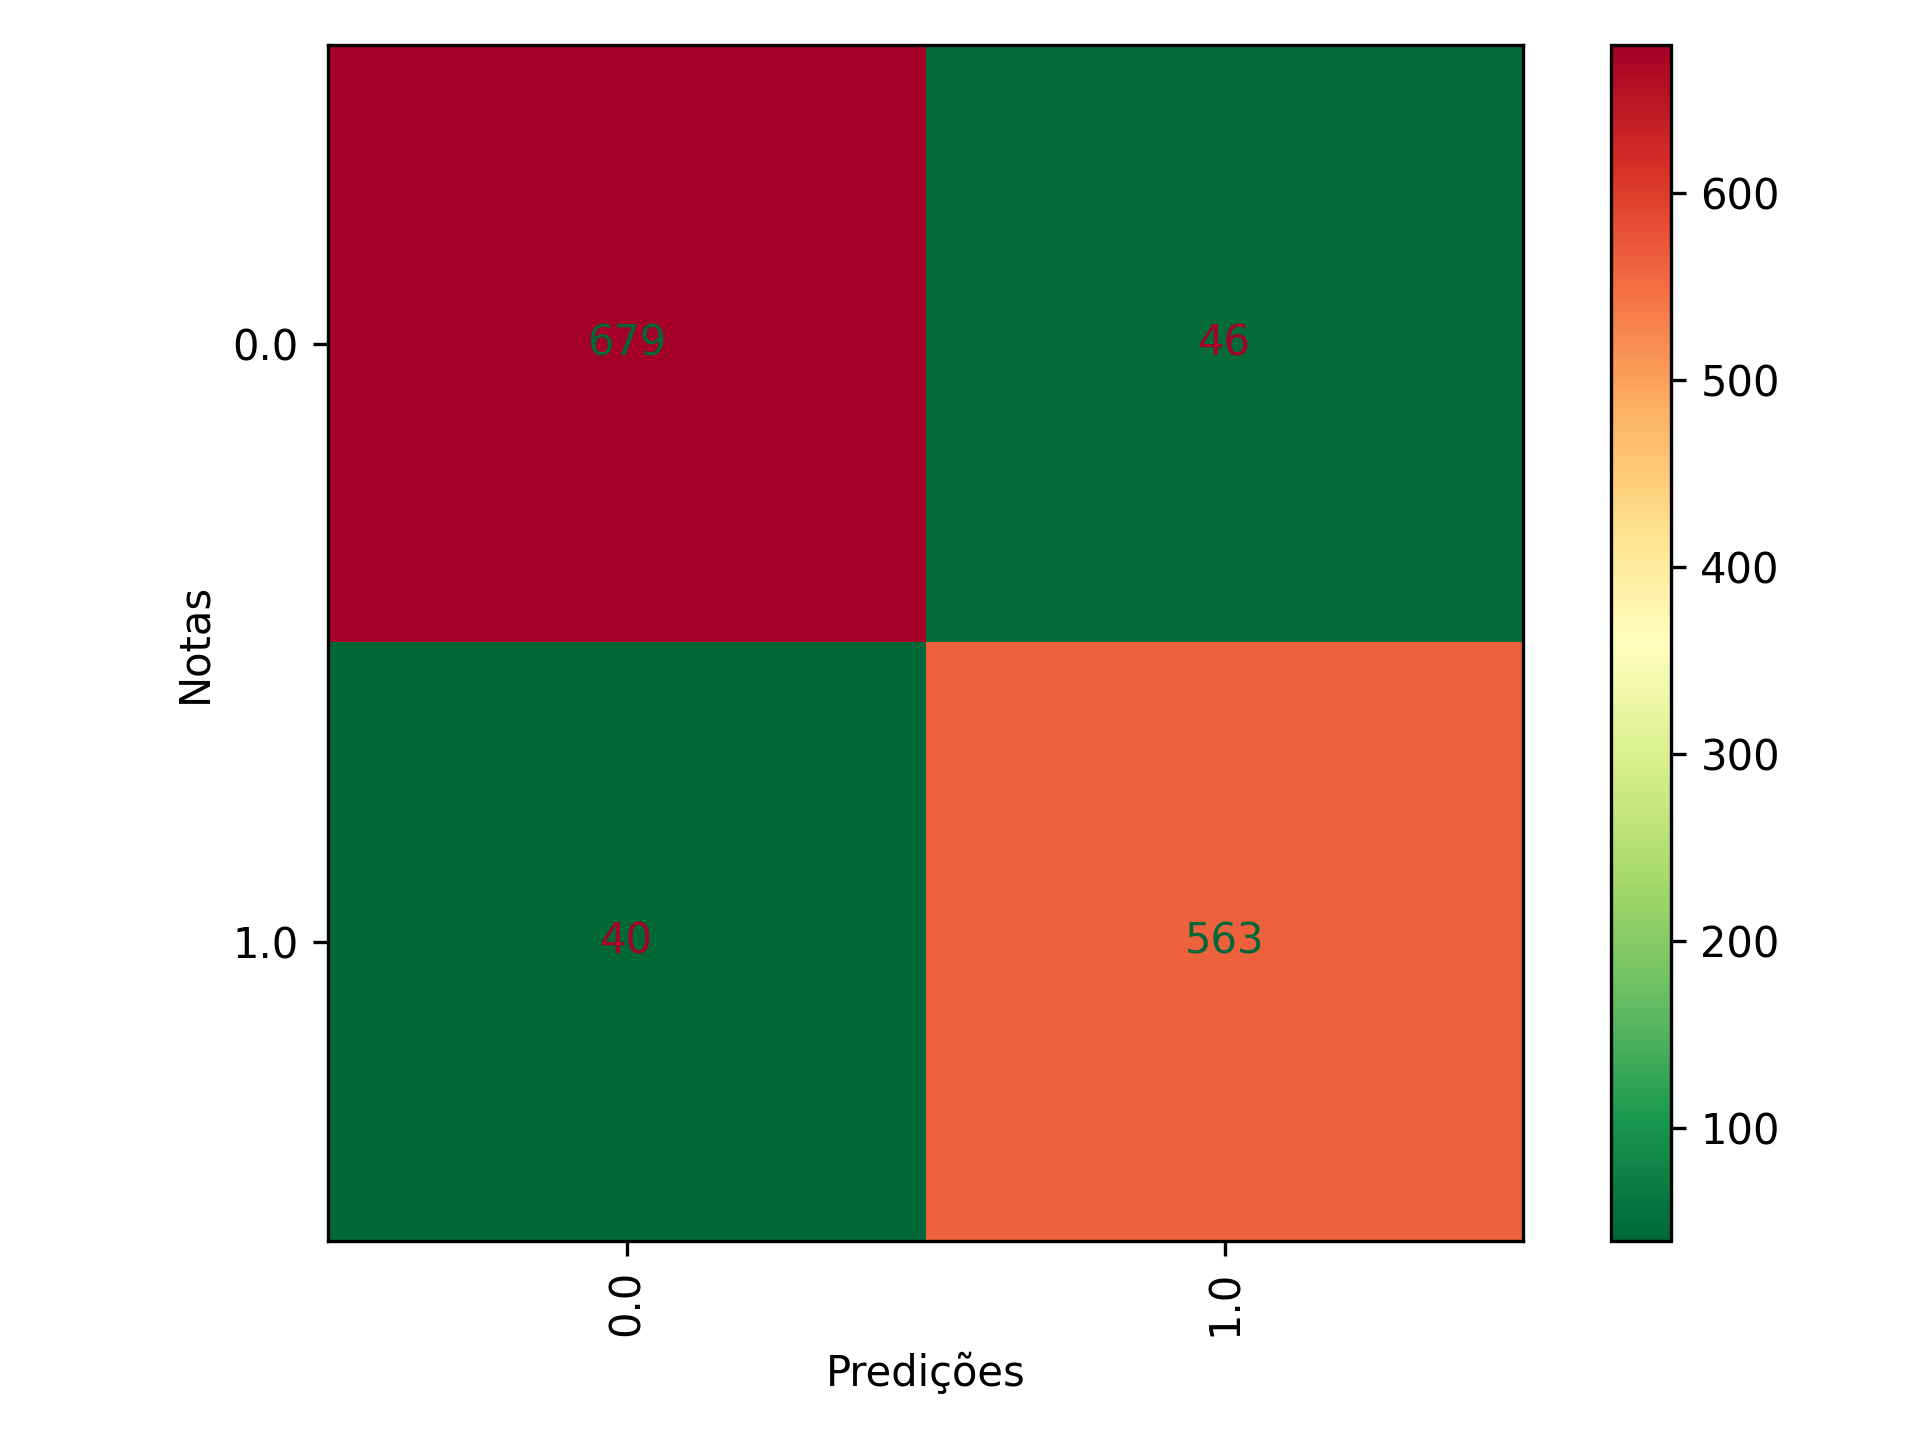
\includegraphics[width=\textwidth]{figuras/exemplo/sandstone-cmGBC.png}
 \caption{GBC}
\end{subfigure}
\hfill
\begin{subfigure}{0.4\textwidth}
 \centering
 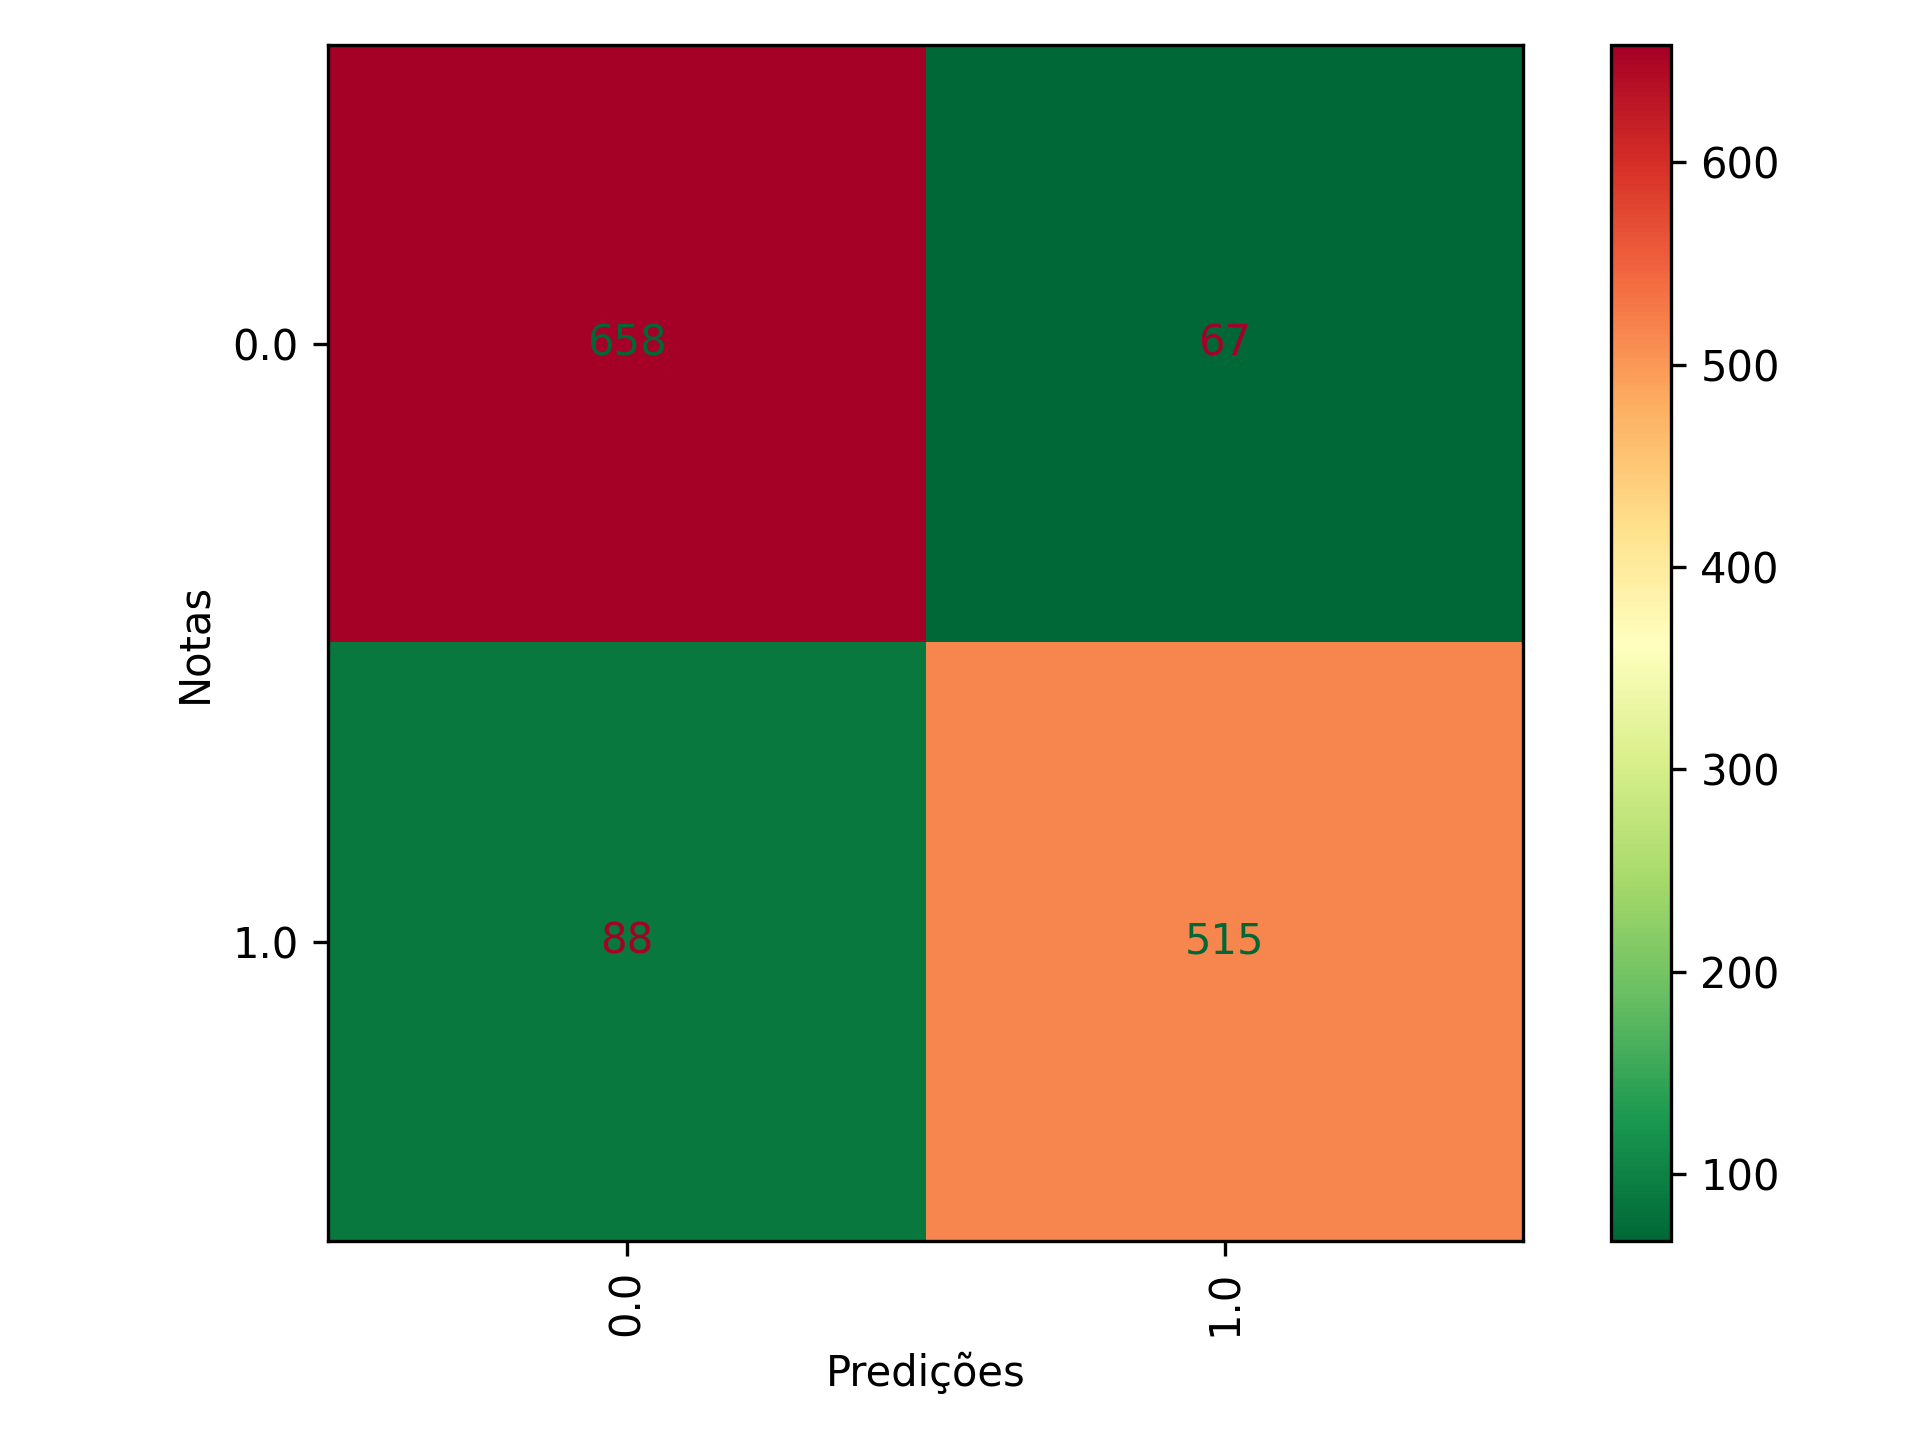
\includegraphics[width=\textwidth]{figuras/exemplo/sandstone-cmRDF.png}
 \caption{RDF}
\end{subfigure}
\caption{Matriz de confusão de todos os 6 algoritmos de classificação para a atividade exemplo.}
\label{fig-exemplo-cm}
\end{figure}


\chapter{Experimentos}

Os conjuntos de dados são representados pela média de todos os resultados observandos em sua série de atividades. Para ilustrar os resultados de toda série de experimentos foram selecionados a partição de treino e teste com 75\% do conjunto de respostas. Nesse aspecto, apresentamos neste capítulo todos os resultados individuais para as atividades de cada base de dados.

\section{UNT}

Atividades da \textit{University of North Texas}

\begin{center} 
	\scriptsize
	\begin{longtable}{l rrr rrr rrr} \\ \hline 
	\multicolumn{10}{l|}{\textbf{University of North Texas}} \\ \hline
	 & \multicolumn{9}{c}{M{\'e}tricas} \\
	M{\'e}todo & MAE & MSE & RMSE & MAE & MSE & RMSE & MAE & MSE & RMSE \\ \hline
	\endhead
	\hline
	\multicolumn{10}{r}{Continua na pr{\'o}xima p{\'a}gina} \\  \hline \hline 
	\endfoot 
	\hline \hline \multicolumn{10}{r}{{\'U}ltima p{\'a}gina} \\ \hline \hline 
	\endlastfoot

	& \multicolumn{9}{c}{\textbf{1.1}} \\ \\
& \multicolumn{3}{l}{A1} & \multicolumn{3}{l}{A2} & \multicolumn{3}{l}{M{\'e}dia} \\ \cline{2-10}

LINR  & 0,4099 & 0,3663 & 0,6052 & 0,6200 & 0,5400 & 0,7400 & 0,4025 & 0,3372 & 0,5807  \\
LSSR  & 1,1131 & 1,4708 & 1,2128 & 1,3800 & 2,1000 & 1,4500 & 1,1488 & 1,6430 & 1,2818  \\
KNRG  & 0,3750 & 0,4028 & 0,6346 & 0,6700 & 0,5600 & 0,7500 & 0,3958 & 0,2326 & 0,4823  \\
DTRG  & 0,2500 & 0,2500 & 0,5000 & 0,7500 & 1,7500 & 1,3200 & 0,6875 & 1,4063 & 1,1859  \\
WSRG  & 0,9922 & 1,1155 & 1,0562 & 1,2000 & 1,5700 & 1,2500 & 0,9792 & 1,1898 & 1,0908  \\
\\ \hline \\
& \multicolumn{9}{c}{\textbf{1.2}} \\ \\
& \multicolumn{3}{l}{A1} & \multicolumn{3}{l}{A2} & \multicolumn{3}{l}{M{\'e}dia} \\ \cline{2-10}

LINR  & 1,0123 & 1,3455 & 1,1599 & 1,2000 & 1,9300 & 1,3900 & 1,1037 & 1,5118 & 1,2295  \\
LSSR  & 0,9881 & 1,4546 & 1,2061 & 1,3100 & 2,1800 & 1,4800 & 1,1488 & 1,6430 & 1,2818  \\
KNRG  & 1,0833 & 1,5833 & 1,2583 & 1,0800 & 1,9200 & 1,3800 & 1,0833 & 1,5833 & 1,2583  \\
DTRG  & 0,6250 & 0,8750 & 0,9354 & 1,6300 & 4,8800 & 2,2100 & 1,0625 & 1,5313 & 1,2374  \\
WSRG  & 0,9784 & 1,4262 & 1,1943 & 1,3300 & 2,2900 & 1,5100 & 1,1581 & 1,6863 & 1,2986  \\
\\ \hline \\
& \multicolumn{9}{c}{\textbf{1.3}} \\ \\
& \multicolumn{3}{l}{A1} & \multicolumn{3}{l}{A2} & \multicolumn{3}{l}{M{\'e}dia} \\ \cline{2-10}

LINR  & 0,1817 & 0,0865 & 0,2942 & 0,2000 & 0,0400 & 0,2100 & 0,1532 & 0,0519 & 0,2279  \\
LSSR  & 0,7440 & 0,6630 & 0,8142 & 0,1300 & 0,1300 & 0,3500 & 0,4345 & 0,2982 & 0,5461  \\
KNRG  & 0,7500 & 0,6111 & 0,7817 & 0,5800 & 0,3900 & 0,6200 & 0,6667 & 0,4444 & 0,6667  \\
DTRG  & 0,1250 & 0,1250 & 0,3536 & 0,6300 & 0,6300 & 0,7900 & 0,8750 & 1,0000 & 1,0000  \\
WSRG  & 0,4734 & 0,3298 & 0,5743 & 0,1800 & 0,0900 & 0,3000 & 0,2456 & 0,1522 & 0,3901  \\
\\ \hline \\
& \multicolumn{9}{c}{\textbf{1.4}} \\ \\
& \multicolumn{3}{l}{A1} & \multicolumn{3}{l}{A2} & \multicolumn{3}{l}{M{\'e}dia} \\ \cline{2-10}

LINR  & 0,6093 & 0,4189 & 0,6472 & 0,2300 & 0,0600 & 0,2400 & 0,3911 & 0,1654 & 0,4067  \\
LSSR  & 0,4762 & 0,2268 & 0,4762 & 0,2400 & 0,0600 & 0,2400 & 0,3571 & 0,1276 & 0,3571  \\
KNRG  & 0,0000 & 0,0000 & 0,0000 & 0,0000 & 0,0000 & 0,0000 & 0,0000 & 0,0000 & 0,0000  \\
DTRG  & 0,0000 & 0,0000 & 0,0000 & 0,0000 & 0,0000 & 0,0000 & 1,8750 & 6,2500 & 2,5000  \\
WSRG  & 0,5916 & 0,3528 & 0,5939 & 0,3300 & 0,1100 & 0,3300 & 0,4709 & 0,2297 & 0,4792  \\
\\ \hline \\
& \multicolumn{9}{c}{\textbf{1.5}} \\ \\
& \multicolumn{3}{l}{A1} & \multicolumn{3}{l}{A2} & \multicolumn{3}{l}{M{\'e}dia} \\ \cline{2-10}

LINR  & 0,7835 & 1,0148 & 1,0074 & 0,1700 & 0,0500 & 0,2200 & 0,3842 & 0,2369 & 0,4867  \\
LSSR  & 1,1488 & 1,4130 & 1,1887 & 0,1900 & 0,0400 & 0,1900 & 0,6220 & 0,4026 & 0,6345  \\
KNRG  & 0,6667 & 1,4722 & 1,2134 & 0,0000 & 0,0000 & 0,0000 & 0,3333 & 0,3681 & 0,6067  \\
DTRG  & 0,8750 & 2,1250 & 1,4577 & 0,0000 & 0,0000 & 0,0000 & 0,3125 & 0,2813 & 0,5303  \\
WSRG  & 1,1383 & 1,3889 & 1,1785 & 0,2600 & 0,0700 & 0,2700 & 0,6260 & 0,4227 & 0,6502  \\
\\ \hline \\
& \multicolumn{9}{c}{\textbf{1.6}} \\ \\
& \multicolumn{3}{l}{A1} & \multicolumn{3}{l}{A2} & \multicolumn{3}{l}{M{\'e}dia} \\ \cline{2-10}

LINR  & 1,2664 & 2,1394 & 1,4627 & 1,0600 & 1,6200 & 1,2700 & 1,1480 & 1,6028 & 1,2660  \\
LSSR  & 1,3750 & 2,6250 & 1,6202 & 1,0700 & 1,9000 & 1,3800 & 1,2232 & 1,9859 & 1,4092  \\
KNRG  & 1,2917 & 2,7361 & 1,6541 & 1,0000 & 1,3900 & 1,1800 & 1,1458 & 1,7465 & 1,3216  \\
DTRG  & 0,7500 & 0,7500 & 0,8660 & 0,7500 & 1,0000 & 1,0000 & 0,6875 & 0,7188 & 0,8478  \\
WSRG  & 1,2882 & 2,1746 & 1,4747 & 0,9600 & 1,5400 & 1,2400 & 1,0739 & 1,5681 & 1,2522  \\
\\ \hline \\
& \multicolumn{9}{c}{\textbf{1.7}} \\ \\
& \multicolumn{3}{l}{A1} & \multicolumn{3}{l}{A2} & \multicolumn{3}{l}{M{\'e}dia} \\ \cline{2-10}

LINR  & 0,4347 & 0,4249 & 0,6518 & 0,2200 & 0,1000 & 0,3200 & 0,2860 & 0,2110 & 0,4593  \\
LSSR  & 0,5893 & 0,4872 & 0,6980 & 0,3700 & 0,1500 & 0,3900 & 0,4405 & 0,2671 & 0,5169  \\
KNRG  & 0,3750 & 0,6250 & 0,7906 & 0,1300 & 0,1300 & 0,3500 & 0,2500 & 0,3125 & 0,5590  \\
DTRG  & 0,3750 & 0,6250 & 0,7906 & 0,1300 & 0,1300 & 0,3500 & 0,2500 & 0,3125 & 0,5590  \\
WSRG  & 0,6966 & 0,5516 & 0,7427 & 0,5100 & 0,2600 & 0,5100 & 0,5573 & 0,3490 & 0,5908  \\
\\ \hline \\
& \multicolumn{9}{c}{\textbf{10.1}} \\ \\
& \multicolumn{3}{l}{A1} & \multicolumn{3}{l}{A2} & \multicolumn{3}{l}{M{\'e}dia} \\ \cline{2-10}

LINR  & 0,5638 & 0,5504 & 0,7419 & 0,2200 & 0,1200 & 0,3500 & 0,3336 & 0,1746 & 0,4179  \\
LSSR  & 0,8148 & 1,0494 & 1,0244 & 0,2400 & 0,1400 & 0,3800 & 0,4537 & 0,3873 & 0,6224  \\
KNRG  & 1,0000 & 1,1481 & 1,0715 & 0,1700 & 0,1700 & 0,4100 & 0,5833 & 0,4120 & 0,6419  \\
DTRG  & 1,1667 & 2,1667 & 1,4720 & 0,1700 & 0,1700 & 0,4100 & 0,9167 & 1,2083 & 1,0992  \\
WSRG  & 0,6499 & 0,8560 & 0,9252 & 0,2500 & 0,1200 & 0,3500 & 0,4184 & 0,2914 & 0,5398  \\
\\ \hline \\
& \multicolumn{9}{c}{\textbf{10.2}} \\ \\
& \multicolumn{3}{l}{A1} & \multicolumn{3}{l}{A2} & \multicolumn{3}{l}{M{\'e}dia} \\ \cline{2-10}

LINR  & 0,5943 & 0,3697 & 0,6080 & 0,2400 & 0,0600 & 0,2500 & 0,4198 & 0,1840 & 0,4290  \\
LSSR  & 1,3333 & 1,7778 & 1,3333 & 0,3300 & 0,1100 & 0,3300 & 0,8333 & 0,6944 & 0,8333  \\
KNRG  & 0,6111 & 0,4630 & 0,6804 & 0,1700 & 0,0600 & 0,2400 & 0,3889 & 0,1944 & 0,4410  \\
DTRG  & 0,0000 & 0,0000 & 0,0000 & 0,0000 & 0,0000 & 0,0000 & 1,2500 & 1,8750 & 1,3693  \\
WSRG  & 1,0883 & 1,1853 & 1,0887 & 0,2500 & 0,0600 & 0,2500 & 0,6771 & 0,4594 & 0,6778  \\
\\ \hline \\
& \multicolumn{9}{c}{\textbf{10.3}} \\ \\
& \multicolumn{3}{l}{A1} & \multicolumn{3}{l}{A2} & \multicolumn{3}{l}{M{\'e}dia} \\ \cline{2-10}

LINR  & 0,0000 & 0,0000 & 0,0000 & 0,0000 & 0,0000 & 0,0000 & 0,0000 & 0,0000 & 0,0000  \\
LSSR  & 0,8889 & 0,7901 & 0,8889 & 0,1100 & 0,0100 & 0,1100 & 0,5000 & 0,2500 & 0,5000  \\
KNRG  & 0,0000 & 0,0000 & 0,0000 & 0,0000 & 0,0000 & 0,0000 & 0,0000 & 0,0000 & 0,0000  \\
DTRG  & 0,0000 & 0,0000 & 0,0000 & 0,0000 & 0,0000 & 0,0000 & 0,0000 & 0,0000 & 0,0000  \\
WSRG  & 0,3419 & 0,1169 & 0,3419 & 0,0500 & 0,0000 & 0,0500 & 0,1955 & 0,0384 & 0,1961  \\
\\ \hline \\
& \multicolumn{9}{c}{\textbf{10.4}} \\ \\
& \multicolumn{3}{l}{A1} & \multicolumn{3}{l}{A2} & \multicolumn{3}{l}{M{\'e}dia} \\ \cline{2-10}

LINR  & 0,4776 & 0,2529 & 0,5029 & 0,0900 & 0,0100 & 0,1100 & 0,2864 & 0,0925 & 0,3042  \\
LSSR  & 0,5556 & 0,3086 & 0,5556 & 0,1100 & 0,0100 & 0,1100 & 0,3333 & 0,1111 & 0,3333  \\
KNRG  & 0,3333 & 0,1111 & 0,3333 & 0,0000 & 0,0000 & 0,0000 & 0,1667 & 0,0278 & 0,1667  \\
DTRG  & 0,5000 & 0,5000 & 0,7071 & 0,0000 & 0,0000 & 0,0000 & 0,0833 & 0,0417 & 0,2041  \\
WSRG  & 0,3508 & 0,1265 & 0,3556 & 0,0700 & 0,0100 & 0,0800 & 0,2188 & 0,0489 & 0,2211  \\
\\ \hline \\
& \multicolumn{9}{c}{\textbf{10.5}} \\ \\
& \multicolumn{3}{l}{A1} & \multicolumn{3}{l}{A2} & \multicolumn{3}{l}{M{\'e}dia} \\ \cline{2-10}

LINR  & 0,9089 & 0,8620 & 0,9284 & 0,6500 & 0,5100 & 0,7100 & 0,7825 & 0,6522 & 0,8076  \\
LSSR  & 1,1667 & 1,5000 & 1,2247 & 0,7000 & 0,6000 & 0,7800 & 0,9352 & 0,9985 & 0,9992  \\
KNRG  & 0,3333 & 0,1111 & 0,3333 & 0,5000 & 0,3900 & 0,6200 & 0,3611 & 0,1528 & 0,3909  \\
DTRG  & 1,1667 & 4,1667 & 2,0412 & 0,8300 & 0,8300 & 0,9100 & 0,8333 & 2,0833 & 1,4434  \\
WSRG  & 1,2418 & 1,5750 & 1,2550 & 0,7700 & 0,6400 & 0,8000 & 1,0103 & 1,0661 & 1,0325  \\
\\ \hline \\
& \multicolumn{9}{c}{\textbf{10.6}} \\ \\
& \multicolumn{3}{l}{A1} & \multicolumn{3}{l}{A2} & \multicolumn{3}{l}{M{\'e}dia} \\ \cline{2-10}

LINR  & 1,0346 & 1,2264 & 1,1074 & 0,4400 & 0,2300 & 0,4800 & 0,6623 & 0,5535 & 0,7439  \\
LSSR  & 1,2037 & 1,7809 & 1,3345 & 0,6100 & 0,3900 & 0,6200 & 0,8426 & 0,8897 & 0,9432  \\
KNRG  & 1,0556 & 1,8333 & 1,3540 & 0,3900 & 0,3900 & 0,6200 & 0,7222 & 0,8796 & 0,9379  \\
DTRG  & 1,5000 & 5,5000 & 2,3452 & 0,1700 & 0,1700 & 0,4100 & 1,0000 & 2,5833 & 1,6073  \\
WSRG  & 1,2254 & 2,0062 & 1,4164 & 0,6700 & 0,4900 & 0,7000 & 0,9010 & 1,0558 & 1,0275  \\
\\ \hline \\
& \multicolumn{9}{c}{\textbf{10.7}} \\ \\
& \multicolumn{3}{l}{A1} & \multicolumn{3}{l}{A2} & \multicolumn{3}{l}{M{\'e}dia} \\ \cline{2-10}

LINR  & 2,2939 & 6,9302 & 2,6325 & 0,5100 & 0,4000 & 0,6300 & 1,3697 & 2,2218 & 1,4906  \\
LSSR  & 2,2037 & 5,5586 & 2,3577 & 0,6100 & 0,3900 & 0,6200 & 1,2963 & 1,7508 & 1,3232  \\
KNRG  & 2,1111 & 7,7778 & 2,7889 & 0,4400 & 0,5600 & 0,7500 & 1,2222 & 2,6204 & 1,6188  \\
DTRG  & 2,8333 & 13,1667 & 3,6286 & 0,6700 & 1,0000 & 1,0000 & 1,9167 & 6,5417 & 2,5577  \\
WSRG  & 2,1879 & 5,6644 & 2,3800 & 0,6700 & 0,5000 & 0,7100 & 1,3286 & 1,8067 & 1,3441  \\
\\ \hline \\
& \multicolumn{9}{c}{\textbf{11.1}} \\ \\
& \multicolumn{3}{l}{A1} & \multicolumn{3}{l}{A2} & \multicolumn{3}{l}{M{\'e}dia} \\ \cline{2-10}

LINR  & 2,1158 & 6,7044 & 2,5893 & 1,6100 & 3,2400 & 1,8000 & 0,7897 & 0,7621 & 0,8730  \\
LSSR  & 2,6705 & 8,8626 & 2,9770 & 2,1500 & 5,3800 & 2,3200 & 1,0284 & 1,1663 & 1,0800  \\
KNRG  & 1,6667 & 6,7778 & 2,6034 & 1,4000 & 3,0000 & 1,7300 & 0,6667 & 0,8403 & 0,9167  \\
DTRG  & 0,8750 & 2,1250 & 1,4577 & 0,8100 & 1,8400 & 1,3600 & 0,3750 & 0,3750 & 0,6124  \\
WSRG  & 2,5181 & 8,8258 & 2,9708 & 2,0900 & 5,0600 & 2,2500 & 0,9877 & 1,0906 & 1,0443  \\
\\ \hline \\
& \multicolumn{9}{c}{\textbf{11.10}} \\ \\
& \multicolumn{3}{l}{A1} & \multicolumn{3}{l}{A2} & \multicolumn{3}{l}{M{\'e}dia} \\ \cline{2-10}

LINR  & 1,0057 & 1,3266 & 1,1518 & 1,0100 & 1,3300 & 1,1500 & 0,2211 & 0,0631 & 0,2512  \\
LSSR  & 0,8182 & 0,6694 & 0,8182 & 0,8200 & 0,6700 & 0,8200 & 0,1818 & 0,0331 & 0,1818  \\
KNRG  & 0,0000 & 0,0000 & 0,0000 & 0,0000 & 0,0000 & 0,0000 & 0,0000 & 0,0000 & 0,0000  \\
DTRG  & 0,7500 & 4,5000 & 2,1213 & 0,8800 & 6,1300 & 2,4700 & 0,1875 & 0,2813 & 0,5303  \\
WSRG  & 1,1894 & 1,4233 & 1,1930 & 1,1700 & 1,3800 & 1,1700 & 0,2603 & 0,0682 & 0,2612  \\
\\ \hline \\
& \multicolumn{9}{c}{\textbf{11.2}} \\ \\
& \multicolumn{3}{l}{A1} & \multicolumn{3}{l}{A2} & \multicolumn{3}{l}{M{\'e}dia} \\ \cline{2-10}

LINR  & 0,4458 & 0,2450 & 0,4949 & 0,4300 & 0,2100 & 0,4500 & 0,2186 & 0,0611 & 0,2472  \\
LSSR  & 1,3636 & 1,8595 & 1,3636 & 1,0300 & 1,0800 & 1,0400 & 0,5455 & 0,2975 & 0,5455  \\
KNRG  & 0,0000 & 0,0000 & 0,0000 & 0,1300 & 0,0600 & 0,2500 & 0,0000 & 0,0000 & 0,0000  \\
DTRG  & 0,0000 & 0,0000 & 0,0000 & 0,1300 & 0,0600 & 0,2500 & 0,0000 & 0,0000 & 0,0000  \\
WSRG  & 1,3046 & 1,7060 & 1,3061 & 1,0200 & 1,0600 & 1,0300 & 0,5517 & 0,3045 & 0,5519  \\
\\ \hline \\
& \multicolumn{9}{c}{\textbf{11.3}} \\ \\
& \multicolumn{3}{l}{A1} & \multicolumn{3}{l}{A2} & \multicolumn{3}{l}{M{\'e}dia} \\ \cline{2-10}

LINR  & 3,1541 & 13,2962 & 3,6464 & 1,4400 & 4,1000 & 2,0300 & 0,7615 & 1,0296 & 1,0147  \\
LSSR  & 2,5682 & 8,4174 & 2,9013 & 1,8600 & 4,9400 & 2,2200 & 0,6761 & 0,6994 & 0,8363  \\
KNRG  & 4,0000 & 19,5556 & 4,4222 & 1,6500 & 6,8400 & 2,6200 & 1,1042 & 2,0590 & 1,4349  \\
DTRG  & 2,5000 & 18,0000 & 4,2426 & 2,9400 & 13,4100 & 3,6600 & 1,4375 & 2,3438 & 1,5309  \\
WSRG  & 2,1943 & 6,4104 & 2,5319 & 2,1200 & 5,6300 & 2,3700 & 0,5240 & 0,5377 & 0,7332  \\
\\ \hline \\
& \multicolumn{9}{c}{\textbf{11.4}} \\ \\
& \multicolumn{3}{l}{A1} & \multicolumn{3}{l}{A2} & \multicolumn{3}{l}{M{\'e}dia} \\ \cline{2-10}

LINR  & 2,5337 & 8,9407 & 2,9901 & 0,7500 & 0,6500 & 0,8100 & 0,5930 & 0,5115 & 0,7152  \\
LSSR  & 2,4886 & 8,4948 & 2,9146 & 0,7800 & 0,6400 & 0,8000 & 0,5852 & 0,4765 & 0,6903  \\
KNRG  & 2,4583 & 11,0139 & 3,3187 & 0,7500 & 0,9200 & 0,9600 & 0,6458 & 0,7674 & 0,8760  \\
DTRG  & 1,8750 & 11,3750 & 3,3727 & 1,6300 & 4,5600 & 2,1400 & 1,0000 & 1,6875 & 1,2990  \\
WSRG  & 2,5430 & 8,5286 & 2,9204 & 0,8800 & 0,7900 & 0,8900 & 0,6335 & 0,4987 & 0,7062  \\
\\ \hline \\
& \multicolumn{9}{c}{\textbf{11.5}} \\ \\
& \multicolumn{3}{l}{A1} & \multicolumn{3}{l}{A2} & \multicolumn{3}{l}{M{\'e}dia} \\ \cline{2-10}

LINR  & 0,8766 & 1,0154 & 1,0077 & 0,5400 & 0,4600 & 0,6800 & 0,3160 & 0,1170 & 0,3420  \\
LSSR  & 0,9318 & 0,8719 & 0,9338 & 0,5500 & 0,3000 & 0,5500 & 0,3182 & 0,1049 & 0,3238  \\
KNRG  & 0,4583 & 0,8472 & 0,9204 & 0,0000 & 0,0000 & 0,0000 & 0,1042 & 0,0451 & 0,2125  \\
DTRG  & 1,0000 & 8,0000 & 2,8284 & 0,0000 & 0,0000 & 0,0000 & 0,5625 & 2,5313 & 1,5910  \\
WSRG  & 1,1376 & 1,3610 & 1,1666 & 0,6700 & 0,4600 & 0,6800 & 0,4205 & 0,1867 & 0,4321  \\
\\ \hline \\
& \multicolumn{9}{c}{\textbf{11.6}} \\ \\
& \multicolumn{3}{l}{A1} & \multicolumn{3}{l}{A2} & \multicolumn{3}{l}{M{\'e}dia} \\ \cline{2-10}

LINR  & 0,2253 & 0,1158 & 0,3403 & 0,5300 & 0,4600 & 0,6800 & 0,1584 & 0,0426 & 0,2065  \\
LSSR  & 0,2273 & 0,0517 & 0,2273 & 0,6400 & 0,4000 & 0,6400 & 0,1818 & 0,0331 & 0,1818  \\
KNRG  & 0,2083 & 0,3472 & 0,5893 & 0,2100 & 0,3500 & 0,5900 & 0,0833 & 0,0556 & 0,2357  \\
DTRG  & 0,0000 & 0,0000 & 0,0000 & 0,6300 & 3,1300 & 1,7700 & 0,1250 & 0,1250 & 0,3536  \\
WSRG  & 0,2004 & 0,0405 & 0,2011 & 0,4200 & 0,1800 & 0,4200 & 0,1267 & 0,0161 & 0,1270  \\
\\ \hline \\
& \multicolumn{9}{c}{\textbf{11.7}} \\ \\
& \multicolumn{3}{l}{A1} & \multicolumn{3}{l}{A2} & \multicolumn{3}{l}{M{\'e}dia} \\ \cline{2-10}

LINR  & 3,4045 & 14,8073 & 3,8480 & 0,3200 & 0,2000 & 0,4500 & 0,8401 & 0,8683 & 0,9318  \\
LSSR  & 4,2273 & 20,9050 & 4,5722 & 0,2000 & 0,2700 & 0,5200 & 1,0114 & 1,1524 & 1,0735  \\
KNRG  & 3,5833 & 15,7778 & 3,9721 & 0,6900 & 0,8000 & 0,8900 & 0,9583 & 1,0347 & 1,0172  \\
DTRG  & 4,1250 & 31,3750 & 5,6013 & 0,9400 & 1,7800 & 1,3300 & 0,5000 & 0,5000 & 0,7071  \\
WSRG  & 3,6914 & 16,4666 & 4,0579 & 0,3700 & 0,3500 & 0,6000 & 0,8440 & 0,8739 & 0,9348  \\
\\ \hline \\
& \multicolumn{9}{c}{\textbf{11.8}} \\ \\
& \multicolumn{3}{l}{A1} & \multicolumn{3}{l}{A2} & \multicolumn{3}{l}{M{\'e}dia} \\ \cline{2-10}

LINR  & 3,4914 & 15,0517 & 3,8796 & 1,3000 & 1,9400 & 1,3900 & 1,0929 & 1,5992 & 1,2646  \\
LSSR  & 3,7614 & 18,3130 & 4,2794 & 1,5500 & 2,5600 & 1,6000 & 1,3580 & 2,0566 & 1,4341  \\
KNRG  & 3,8333 & 25,3333 & 5,0332 & 1,5800 & 3,1700 & 1,7800 & 1,2917 & 2,7014 & 1,6436  \\
DTRG  & 1,7500 & 7,5000 & 2,7386 & 1,5600 & 3,3400 & 1,8300 & 0,5625 & 0,6563 & 0,8101  \\
WSRG  & 3,5744 & 16,7159 & 4,0885 & 1,4400 & 2,3000 & 1,5200 & 1,2580 & 1,8765 & 1,3699  \\
\\ \hline \\
& \multicolumn{9}{c}{\textbf{11.9}} \\ \\
& \multicolumn{3}{l}{A1} & \multicolumn{3}{l}{A2} & \multicolumn{3}{l}{M{\'e}dia} \\ \cline{2-10}

LINR  & 0,5870 & 0,4736 & 0,6882 & 0,1600 & 0,0300 & 0,1800 & 0,2180 & 0,0783 & 0,2798  \\
LSSR  & 0,8068 & 0,7603 & 0,8720 & 0,1600 & 0,0300 & 0,1600 & 0,2898 & 0,1113 & 0,3336  \\
KNRG  & 0,6250 & 0,6250 & 0,7906 & 0,2900 & 0,0900 & 0,3000 & 0,1250 & 0,0347 & 0,1863  \\
DTRG  & 2,5000 & 9,7500 & 3,1225 & 0,6300 & 0,6300 & 0,7900 & 0,5625 & 0,4063 & 0,6374  \\
WSRG  & 0,9529 & 1,0122 & 1,0061 & 0,0700 & 0,0100 & 0,0700 & 0,3265 & 0,1378 & 0,3713  \\
\\ \hline \\
& \multicolumn{9}{c}{\textbf{12.1}} \\ \\
& \multicolumn{3}{l}{A1} & \multicolumn{3}{l}{A2} & \multicolumn{3}{l}{M{\'e}dia} \\ \cline{2-10}

LINR  & 1,3203 & 5,6592 & 2,3789 & 0,0400 & 0,0000 & 0,0600 & 0,3252 & 0,3738 & 0,6114  \\
LSSR  & 1,5102 & 8,2132 & 2,8659 & 0,0700 & 0,0100 & 0,0700 & 0,3707 & 0,5176 & 0,7194  \\
KNRG  & 0,9048 & 4,6190 & 2,1492 & 0,0700 & 0,0400 & 0,1900 & 0,2619 & 0,3373 & 0,5808  \\
DTRG  & 1,4286 & 9,4286 & 3,0706 & 0,0000 & 0,0000 & 0,0000 & 0,0714 & 0,0357 & 0,1890  \\
WSRG  & 1,4695 & 7,5071 & 2,7399 & 0,0900 & 0,0100 & 0,0900 & 0,3847 & 0,4869 & 0,6978  \\
\\ \hline \\
& \multicolumn{9}{c}{\textbf{12.10}} \\ \\
& \multicolumn{3}{l}{A1} & \multicolumn{3}{l}{A2} & \multicolumn{3}{l}{M{\'e}dia} \\ \cline{2-10}

LINR  & 3,8698 & 16,6488 & 4,0803 & 1,2500 & 1,7600 & 1,3300 & 1,2352 & 1,7781 & 1,3334  \\
LSSR  & 3,5442 & 14,5737 & 3,8176 & 1,3600 & 1,8400 & 1,3600 & 1,2857 & 1,7755 & 1,3325  \\
KNRG  & 4,2857 & 20,9524 & 4,5774 & 1,3800 & 2,3600 & 1,5400 & 1,4286 & 2,2619 & 1,5040  \\
DTRG  & 2,1429 & 17,8571 & 4,2258 & 1,1400 & 4,5700 & 2,1400 & 1,1429 & 3,6429 & 1,9086  \\
WSRG  & 3,5405 & 14,2504 & 3,7750 & 1,2900 & 1,6800 & 1,3000 & 1,2469 & 1,6961 & 1,3024  \\
\\ \hline \\
& \multicolumn{9}{c}{\textbf{12.2}} \\ \\
& \multicolumn{3}{l}{A1} & \multicolumn{3}{l}{A2} & \multicolumn{3}{l}{M{\'e}dia} \\ \cline{2-10}

LINR  & 2,8727 & 9,7189 & 3,1175 & 1,0200 & 1,6500 & 1,2800 & 0,8079 & 0,8298 & 0,9109  \\
LSSR  & 2,7415 & 8,4512 & 2,9071 & 1,0700 & 2,0400 & 1,4300 & 0,7075 & 0,7336 & 0,8565  \\
KNRG  & 2,2857 & 10,0000 & 3,1623 & 1,1700 & 1,7300 & 1,3100 & 0,6429 & 0,6944 & 0,8333  \\
DTRG  & 2,2857 & 11,7143 & 3,4226 & 1,0000 & 1,7100 & 1,3100 & 1,5000 & 2,4643 & 1,5698  \\
WSRG  & 2,8682 & 10,1307 & 3,1829 & 1,6500 & 3,6300 & 1,9000 & 0,8761 & 1,0963 & 1,0471  \\
\\ \hline \\
& \multicolumn{9}{c}{\textbf{12.3}} \\ \\
& \multicolumn{3}{l}{A1} & \multicolumn{3}{l}{A2} & \multicolumn{3}{l}{M{\'e}dia} \\ \cline{2-10}

LINR  & 2,3451 & 6,6527 & 2,5793 & 0,4400 & 0,3300 & 0,5700 & 0,6863 & 0,6035 & 0,7769  \\
LSSR  & 3,1905 & 10,9955 & 3,3159 & 1,1600 & 1,6900 & 1,3000 & 1,0536 & 1,2905 & 1,1360  \\
KNRG  & 2,5714 & 7,4286 & 2,7255 & 0,9000 & 0,8500 & 0,9200 & 0,8690 & 0,8209 & 0,9061  \\
DTRG  & 2,4286 & 11,0000 & 3,3166 & 1,3600 & 2,1800 & 1,4800 & 1,4107 & 2,0558 & 1,4338  \\
WSRG  & 3,4947 & 12,3186 & 3,5098 & 1,0000 & 1,2300 & 1,1100 & 1,2095 & 1,5382 & 1,2402  \\
\\ \hline \\
& \multicolumn{9}{c}{\textbf{12.4}} \\ \\
& \multicolumn{3}{l}{A1} & \multicolumn{3}{l}{A2} & \multicolumn{3}{l}{M{\'e}dia} \\ \cline{2-10}

LINR  & 3,3970 & 12,3565 & 3,5152 & 0,8000 & 0,8300 & 0,9100 & 0,9074 & 0,9882 & 0,9941  \\
LSSR  & 3,7143 & 13,7959 & 3,7143 & 0,9100 & 1,1700 & 1,0800 & 1,0238 & 1,1094 & 1,0533  \\
KNRG  & 1,1429 & 3,0476 & 1,7457 & 0,9800 & 1,1100 & 1,0500 & 0,4524 & 0,2976 & 0,5455  \\
DTRG  & 1,1429 & 9,1429 & 3,0237 & 1,2900 & 2,5700 & 1,6000 & 0,0714 & 0,0357 & 0,1890  \\
WSRG  & 3,2987 & 10,8947 & 3,3007 & 0,8800 & 1,1400 & 1,0700 & 0,9084 & 0,8895 & 0,9431  \\
\\ \hline \\
& \multicolumn{9}{c}{\textbf{12.5}} \\ \\
& \multicolumn{3}{l}{A1} & \multicolumn{3}{l}{A2} & \multicolumn{3}{l}{M{\'e}dia} \\ \cline{2-10}

LINR  & 0,1996 & 0,0451 & 0,2125 & 0,2000 & 0,0500 & 0,2100 & 0,0408 & 0,0021 & 0,0453  \\
LSSR  & 0,1429 & 0,0204 & 0,1429 & 0,1400 & 0,0200 & 0,1400 & 0,0238 & 0,0006 & 0,0238  \\
KNRG  & 0,3333 & 0,2063 & 0,4543 & 0,3300 & 0,2100 & 0,4500 & 0,0714 & 0,0119 & 0,1091  \\
DTRG  & 0,0000 & 0,0000 & 0,0000 & 0,0000 & 0,0000 & 0,0000 & 0,0000 & 0,0000 & 0,0000  \\
WSRG  & 0,0939 & 0,0089 & 0,0941 & 0,0900 & 0,0100 & 0,0900 & 0,0158 & 0,0003 & 0,0158  \\
\\ \hline \\
& \multicolumn{9}{c}{\textbf{12.6}} \\ \\
& \multicolumn{3}{l}{A1} & \multicolumn{3}{l}{A2} & \multicolumn{3}{l}{M{\'e}dia} \\ \cline{2-10}

LINR  & 0,3505 & 0,1884 & 0,4341 & 0,7800 & 3,4900 & 1,8700 & 0,2316 & 0,1547 & 0,3933  \\
LSSR  & 1,3810 & 1,9070 & 1,3810 & 0,8800 & 3,2900 & 1,8100 & 0,4150 & 0,1791 & 0,4232  \\
KNRG  & 0,0000 & 0,0000 & 0,0000 & 0,7100 & 3,5700 & 1,8900 & 0,1429 & 0,1429 & 0,3780  \\
DTRG  & 0,0000 & 0,0000 & 0,0000 & 0,7100 & 3,5700 & 1,8900 & 0,1429 & 0,1429 & 0,3780  \\
WSRG  & 1,6368 & 2,6858 & 1,6388 & 0,9300 & 3,2500 & 1,8000 & 0,4715 & 0,2248 & 0,4742  \\
\\ \hline \\
& \multicolumn{9}{c}{\textbf{12.7}} \\ \\
& \multicolumn{3}{l}{A1} & \multicolumn{3}{l}{A2} & \multicolumn{3}{l}{M{\'e}dia} \\ \cline{2-10}

LINR  & 0,0000 & 0,0000 & 0,0000 & 0,0000 & 0,0000 & 0,0000 & 0,0000 & 0,0000 & 0,0000  \\
LSSR  & 0,1905 & 0,0363 & 0,1905 & 0,1900 & 0,0400 & 0,1900 & 0,0238 & 0,0006 & 0,0238  \\
KNRG  & 0,0000 & 0,0000 & 0,0000 & 0,0000 & 0,0000 & 0,0000 & 0,0000 & 0,0000 & 0,0000  \\
DTRG  & 0,0000 & 0,0000 & 0,0000 & 0,0000 & 0,0000 & 0,0000 & 0,0000 & 0,0000 & 0,0000  \\
WSRG  & 0,1749 & 0,0306 & 0,1749 & 0,1700 & 0,0300 & 0,1700 & 0,0333 & 0,0011 & 0,0333  \\
\\ \hline \\
& \multicolumn{9}{c}{\textbf{12.8}} \\ \\
& \multicolumn{3}{l}{A1} & \multicolumn{3}{l}{A2} & \multicolumn{3}{l}{M{\'e}dia} \\ \cline{2-10}

LINR  & 2,4115 & 9,0905 & 3,0150 & 1,0700 & 1,3700 & 1,1700 & 0,7580 & 0,8569 & 0,9257  \\
LSSR  & 2,6667 & 10,3492 & 3,2170 & 1,3600 & 2,3200 & 1,5200 & 0,8707 & 1,1519 & 1,0733  \\
KNRG  & 3,1429 & 14,1270 & 3,7586 & 1,3800 & 2,1900 & 1,4800 & 0,9524 & 1,2222 & 1,1055  \\
DTRG  & 2,1429 & 9,0000 & 3,0000 & 0,7100 & 0,9300 & 0,9600 & 0,8571 & 1,1429 & 1,0690  \\
WSRG  & 2,7338 & 9,8338 & 3,1359 & 1,3800 & 2,3900 & 1,5500 & 0,8702 & 1,1198 & 1,0582  \\
\\ \hline \\
& \multicolumn{9}{c}{\textbf{12.9}} \\ \\
& \multicolumn{3}{l}{A1} & \multicolumn{3}{l}{A2} & \multicolumn{3}{l}{M{\'e}dia} \\ \cline{2-10}

LINR  & 3,8243 & 16,4647 & 4,0577 & 0,8300 & 1,3000 & 1,1400 & 1,0749 & 1,3632 & 1,1676  \\
LSSR  & 4,3537 & 20,4989 & 4,5276 & 1,0900 & 2,1100 & 1,4500 & 1,2925 & 1,8730 & 1,3686  \\
KNRG  & 3,2857 & 16,6825 & 4,0844 & 1,2900 & 2,1700 & 1,4700 & 1,0000 & 1,8175 & 1,3481  \\
DTRG  & 3,4286 & 15,7143 & 3,9641 & 0,7900 & 1,5400 & 1,2400 & 1,1429 & 2,1429 & 1,4639  \\
WSRG  & 4,4164 & 22,3348 & 4,7260 & 1,4100 & 2,9600 & 1,7200 & 1,3086 & 2,0614 & 1,4358  \\
\\ \hline \\
& \multicolumn{9}{c}{\textbf{2.1}} \\ \\
& \multicolumn{3}{l}{A1} & \multicolumn{3}{l}{A2} & \multicolumn{3}{l}{M{\'e}dia} \\ \cline{2-10}

LINR  & 0,7424 & 1,1739 & 1,0835 & 0,3700 & 0,3000 & 0,5500 & 0,4524 & 0,5808 & 0,7621  \\
LSSR  & 1,2273 & 1,9959 & 1,4128 & 0,6300 & 0,4900 & 0,7000 & 0,8068 & 0,9788 & 0,9894  \\
KNRG  & 0,5000 & 1,4444 & 1,2019 & 0,5000 & 0,5300 & 0,7300 & 0,5000 & 0,8542 & 0,9242  \\
DTRG  & 0,5000 & 1,2500 & 1,1180 & 0,1300 & 0,1300 & 0,3500 & 0,2500 & 0,5000 & 0,7071  \\
WSRG  & 1,1674 & 1,8467 & 1,3589 & 0,5700 & 0,4200 & 0,6500 & 0,7506 & 0,8430 & 0,9182  \\
\\ \hline \\
& \multicolumn{9}{c}{\textbf{2.2}} \\ \\
& \multicolumn{3}{l}{A1} & \multicolumn{3}{l}{A2} & \multicolumn{3}{l}{M{\'e}dia} \\ \cline{2-10}

LINR  & 1,2575 & 2,4373 & 1,5612 & 0,3800 & 0,2500 & 0,5000 & 0,5849 & 0,6973 & 0,8351  \\
LSSR  & 1,3295 & 2,7831 & 1,6682 & 0,4100 & 0,2900 & 0,5400 & 0,6193 & 0,8215 & 0,9064  \\
KNRG  & 1,5000 & 3,3889 & 1,8409 & 0,4200 & 0,2800 & 0,5300 & 0,7917 & 1,0139 & 1,0069  \\
DTRG  & 1,6250 & 4,3750 & 2,0917 & 0,2500 & 0,2500 & 0,5000 & 1,0625 & 2,0313 & 1,4252  \\
WSRG  & 1,2952 & 2,7708 & 1,6646 & 0,4100 & 0,2900 & 0,5400 & 0,6031 & 0,8114 & 0,9008  \\
\\ \hline \\
& \multicolumn{9}{c}{\textbf{2.3}} \\ \\
& \multicolumn{3}{l}{A1} & \multicolumn{3}{l}{A2} & \multicolumn{3}{l}{M{\'e}dia} \\ \cline{2-10}

LINR  & 0,7580 & 0,7313 & 0,8552 & 0,6900 & 0,7300 & 0,8500 & 0,5122 & 0,3437 & 0,5863  \\
LSSR  & 0,9659 & 1,2004 & 1,0956 & 0,7700 & 0,8500 & 0,9200 & 0,5511 & 0,4680 & 0,6841  \\
KNRG  & 0,7917 & 1,0139 & 1,0069 & 0,6300 & 0,7100 & 0,8400 & 0,7083 & 0,6736 & 0,8207  \\
DTRG  & 1,3750 & 2,1250 & 1,4577 & 0,3800 & 0,3800 & 0,6100 & 0,6250 & 0,6250 & 0,7906  \\
WSRG  & 0,9988 & 1,1968 & 1,0940 & 0,7000 & 0,7500 & 0,8700 & 0,5225 & 0,4005 & 0,6329  \\
\\ \hline \\
& \multicolumn{9}{c}{\textbf{2.4}} \\ \\
& \multicolumn{3}{l}{A1} & \multicolumn{3}{l}{A2} & \multicolumn{3}{l}{M{\'e}dia} \\ \cline{2-10}

LINR  & 0,4294 & 0,2428 & 0,4927 & 0,1800 & 0,0500 & 0,2300 & 0,3086 & 0,1334 & 0,3652  \\
LSSR  & 0,7727 & 0,5971 & 0,7727 & 0,3600 & 0,1300 & 0,3600 & 0,5682 & 0,3228 & 0,5682  \\
KNRG  & 0,0833 & 0,0556 & 0,2357 & 0,0800 & 0,0600 & 0,2400 & 0,0833 & 0,0556 & 0,2357  \\
DTRG  & 0,0000 & 0,0000 & 0,0000 & 0,0000 & 0,0000 & 0,0000 & 0,0000 & 0,0000 & 0,0000  \\
WSRG  & 0,8200 & 0,6794 & 0,8243 & 0,3300 & 0,1100 & 0,3300 & 0,5508 & 0,3100 & 0,5568  \\
\\ \hline \\
& \multicolumn{9}{c}{\textbf{2.5}} \\ \\
& \multicolumn{3}{l}{A1} & \multicolumn{3}{l}{A2} & \multicolumn{3}{l}{M{\'e}dia} \\ \cline{2-10}

LINR  & 1,3432 & 2,5149 & 1,5859 & 0,8600 & 1,1800 & 1,0900 & 1,0639 & 1,6266 & 1,2754  \\
LSSR  & 1,9318 & 3,7459 & 1,9354 & 1,5100 & 2,4000 & 1,5500 & 1,6364 & 2,7960 & 1,6721  \\
KNRG  & 1,0000 & 2,0556 & 1,4337 & 0,5000 & 0,8100 & 0,9000 & 0,7500 & 1,2431 & 1,1149  \\
DTRG  & 1,0000 & 4,0000 & 2,0000 & 1,0000 & 2,2500 & 1,5000 & 0,7500 & 2,3125 & 1,5207  \\
WSRG  & 2,1447 & 4,7530 & 2,1801 & 1,9400 & 4,1300 & 2,0300 & 1,8760 & 4,1829 & 2,0452  \\
\\ \hline \\
& \multicolumn{9}{c}{\textbf{2.6}} \\ \\
& \multicolumn{3}{l}{A1} & \multicolumn{3}{l}{A2} & \multicolumn{3}{l}{M{\'e}dia} \\ \cline{2-10}

LINR  & 0,5807 & 0,3864 & 0,6216 & 0,3200 & 0,1600 & 0,4000 & 0,3454 & 0,1568 & 0,3959  \\
LSSR  & 0,6250 & 0,6250 & 0,7906 & 0,3900 & 0,3400 & 0,5900 & 0,4886 & 0,3528 & 0,5940  \\
KNRG  & 0,5833 & 0,6111 & 0,7817 & 0,3300 & 0,1900 & 0,4400 & 0,3750 & 0,2431 & 0,4930  \\
DTRG  & 1,1250 & 3,3750 & 1,8371 & 0,2500 & 0,2500 & 0,5000 & 0,3750 & 0,2500 & 0,5000  \\
WSRG  & 0,5871 & 0,4694 & 0,6851 & 0,3700 & 0,3400 & 0,5900 & 0,4607 & 0,3110 & 0,5576  \\
\\ \hline \\
& \multicolumn{9}{c}{\textbf{2.7}} \\ \\
& \multicolumn{3}{l}{A1} & \multicolumn{3}{l}{A2} & \multicolumn{3}{l}{M{\'e}dia} \\ \cline{2-10}

LINR  & 1,3229 & 2,4271 & 1,5579 & 0,5200 & 0,3400 & 0,5800 & 0,7363 & 0,8278 & 0,9098  \\
LSSR  & 1,5000 & 3,0000 & 1,7321 & 0,4100 & 0,2900 & 0,5400 & 0,8864 & 1,0217 & 1,0108  \\
KNRG  & 0,8750 & 1,5139 & 1,2304 & 0,6700 & 0,5600 & 0,7500 & 0,6458 & 0,6563 & 0,8101  \\
DTRG  & 2,5000 & 8,0000 & 2,8284 & 1,5000 & 2,7500 & 1,6600 & 1,4375 & 3,2188 & 1,7941  \\
WSRG  & 1,5978 & 3,2000 & 1,7888 & 0,3900 & 0,3500 & 0,5900 & 0,9730 & 1,1423 & 1,0688  \\
\\ \hline \\
& \multicolumn{9}{c}{\textbf{3.1}} \\ \\
& \multicolumn{3}{l}{A1} & \multicolumn{3}{l}{A2} & \multicolumn{3}{l}{M{\'e}dia} \\ \cline{2-10}

LINR  & 0,4077 & 0,2882 & 0,5369 & 0,0200 & 0,0000 & 0,0400 & 0,2016 & 0,0747 & 0,2733  \\
LSSR  & 1,1739 & 1,3781 & 1,1739 & 0,0900 & 0,0100 & 0,0900 & 0,6304 & 0,3974 & 0,6304  \\
KNRG  & 0,0000 & 0,0000 & 0,0000 & 0,0000 & 0,0000 & 0,0000 & 0,0000 & 0,0000 & 0,0000  \\
DTRG  & 0,1250 & 0,1250 & 0,3536 & 0,0000 & 0,0000 & 0,0000 & 0,0625 & 0,0313 & 0,1768  \\
WSRG  & 0,7787 & 0,6222 & 0,7888 & 0,0400 & 0,0000 & 0,0400 & 0,3927 & 0,1584 & 0,3981  \\
\\ \hline \\
& \multicolumn{9}{c}{\textbf{3.2}} \\ \\
& \multicolumn{3}{l}{A1} & \multicolumn{3}{l}{A2} & \multicolumn{3}{l}{M{\'e}dia} \\ \cline{2-10}

LINR  & 0,9677 & 1,4515 & 1,2048 & 1,1900 & 1,7600 & 1,3300 & 0,4730 & 0,3416 & 0,5845  \\
LSSR  & 1,0707 & 1,2691 & 1,1266 & 1,2600 & 1,5900 & 1,2600 & 0,5353 & 0,3173 & 0,5633  \\
KNRG  & 0,9583 & 2,0972 & 1,4482 & 1,3300 & 2,7200 & 1,6500 & 0,4792 & 0,5243 & 0,7241  \\
DTRG  & 1,6250 & 7,3750 & 2,7157 & 2,0000 & 9,5000 & 3,0800 & 0,8125 & 1,8438 & 1,3578  \\
WSRG  & 0,9202 & 0,9887 & 0,9943 & 1,0500 & 1,1300 & 1,0600 & 0,4631 & 0,2510 & 0,5010  \\
\\ \hline \\
& \multicolumn{9}{c}{\textbf{3.3}} \\ \\
& \multicolumn{3}{l}{A1} & \multicolumn{3}{l}{A2} & \multicolumn{3}{l}{M{\'e}dia} \\ \cline{2-10}

LINR  & 1,2649 & 2,8550 & 1,6897 & 0,9100 & 1,4700 & 1,2100 & 0,9681 & 1,5251 & 1,2350  \\
LSSR  & 1,7935 & 4,4750 & 2,1154 & 1,1700 & 2,1300 & 1,4600 & 1,4130 & 2,7395 & 1,6551  \\
KNRG  & 1,1667 & 2,2222 & 1,4907 & 1,1700 & 2,3100 & 1,5200 & 1,0000 & 1,7361 & 1,3176  \\
DTRG  & 1,5000 & 4,7500 & 2,1794 & 1,0000 & 1,5000 & 1,2200 & 1,3125 & 3,2813 & 1,8114  \\
WSRG  & 1,5709 & 3,3694 & 1,8356 & 0,9500 & 1,5700 & 1,2500 & 1,2198 & 1,9614 & 1,4005  \\
\\ \hline \\
& \multicolumn{9}{c}{\textbf{3.4}} \\ \\
& \multicolumn{3}{l}{A1} & \multicolumn{3}{l}{A2} & \multicolumn{3}{l}{M{\'e}dia} \\ \cline{2-10}

LINR  & 0,6930 & 0,5564 & 0,7459 & 0,6400 & 0,5400 & 0,7300 & 0,6643 & 0,5166 & 0,7187  \\
LSSR  & 1,0000 & 1,0000 & 1,0000 & 0,7500 & 0,6900 & 0,8300 & 0,8750 & 0,7983 & 0,8935  \\
KNRG  & 1,0417 & 1,2639 & 1,1242 & 0,8800 & 1,1000 & 1,0500 & 0,9583 & 1,1597 & 1,0769  \\
DTRG  & 0,3750 & 0,6250 & 0,7906 & 0,6300 & 0,8800 & 0,9400 & 0,0625 & 0,0313 & 0,1768  \\
WSRG  & 0,9493 & 0,9099 & 0,9539 & 0,7300 & 0,6600 & 0,8100 & 0,8418 & 0,7539 & 0,8683  \\
\\ \hline \\
& \multicolumn{9}{c}{\textbf{3.5}} \\ \\
& \multicolumn{3}{l}{A1} & \multicolumn{3}{l}{A2} & \multicolumn{3}{l}{M{\'e}dia} \\ \cline{2-10}

LINR  & 0,4770 & 0,4571 & 0,6761 & 0,1900 & 0,0500 & 0,2200 & 0,3345 & 0,1961 & 0,4428  \\
LSSR  & 1,2609 & 1,5898 & 1,2609 & 0,5200 & 0,2700 & 0,5200 & 0,8913 & 0,7944 & 0,8913  \\
KNRG  & 0,1667 & 0,1111 & 0,3333 & 0,0000 & 0,0000 & 0,0000 & 0,0833 & 0,0278 & 0,1667  \\
DTRG  & 0,7500 & 2,2500 & 1,5000 & 0,0000 & 0,0000 & 0,0000 & 0,0000 & 0,0000 & 0,0000  \\
WSRG  & 1,0349 & 1,1112 & 1,0541 & 0,5100 & 0,2600 & 0,5100 & 0,7263 & 0,5507 & 0,7421  \\
\\ \hline \\
& \multicolumn{9}{c}{\textbf{3.6}} \\ \\
& \multicolumn{3}{l}{A1} & \multicolumn{3}{l}{A2} & \multicolumn{3}{l}{M{\'e}dia} \\ \cline{2-10}

LINR  & 0,4473 & 0,2482 & 0,4982 & 0,0100 & 0,0000 & 0,0200 & 0,2289 & 0,0654 & 0,2557  \\
LSSR  & 0,9130 & 0,8336 & 0,9130 & 0,0900 & 0,0100 & 0,0900 & 0,5000 & 0,2500 & 0,5000  \\
KNRG  & 0,1667 & 0,1389 & 0,3727 & 0,0000 & 0,0000 & 0,0000 & 0,0833 & 0,0347 & 0,1863  \\
DTRG  & 0,0000 & 0,0000 & 0,0000 & 0,0000 & 0,0000 & 0,0000 & 0,0625 & 0,0313 & 0,1768  \\
WSRG  & 0,7443 & 0,5604 & 0,7486 & 0,0800 & 0,0100 & 0,0800 & 0,4006 & 0,1630 & 0,4037  \\
\\ \hline \\
& \multicolumn{9}{c}{\textbf{3.7}} \\ \\
& \multicolumn{3}{l}{A1} & \multicolumn{3}{l}{A2} & \multicolumn{3}{l}{M{\'e}dia} \\ \cline{2-10}

LINR  & 0,8118 & 0,9148 & 0,9565 & 0,3500 & 0,2400 & 0,4900 & 0,5764 & 0,4483 & 0,6696  \\
LSSR  & 1,3587 & 1,9060 & 1,3806 & 0,5300 & 0,2900 & 0,5400 & 0,9457 & 0,9031 & 0,9503  \\
KNRG  & 0,7500 & 2,2500 & 1,5000 & 0,2500 & 0,2500 & 0,5000 & 0,5000 & 1,0000 & 1,0000  \\
DTRG  & 0,7500 & 2,2500 & 1,5000 & 0,5000 & 0,7500 & 0,8700 & 1,0000 & 2,5000 & 1,5811  \\
WSRG  & 1,2888 & 1,6982 & 1,3032 & 0,5500 & 0,3700 & 0,6100 & 0,9054 & 0,8331 & 0,9127  \\
\\ \hline \\
& \multicolumn{9}{c}{\textbf{4.2}} \\ \\
& \multicolumn{3}{l}{A1} & \multicolumn{3}{l}{A2} & \multicolumn{3}{l}{M{\'e}dia} \\ \cline{2-10}

LINR  & 1,2413 & 1,9135 & 1,3833 & 0,3100 & 0,1200 & 0,3500 & 0,6552 & 0,5730 & 0,7570  \\
LSSR  & 1,4091 & 2,3595 & 1,5361 & 0,3600 & 0,1500 & 0,3800 & 0,7500 & 0,7583 & 0,8708  \\
KNRG  & 0,9167 & 1,2500 & 1,1180 & 0,5000 & 0,3300 & 0,5800 & 0,6250 & 0,5556 & 0,7454  \\
DTRG  & 1,5000 & 3,7500 & 1,9365 & 0,1300 & 0,1300 & 0,3500 & 0,8125 & 1,2188 & 1,1040  \\
WSRG  & 1,3864 & 2,3319 & 1,5271 & 0,3200 & 0,1300 & 0,3600 & 0,7401 & 0,7442 & 0,8627  \\
\\ \hline \\
& \multicolumn{9}{c}{\textbf{4.3}} \\ \\
& \multicolumn{3}{l}{A1} & \multicolumn{3}{l}{A2} & \multicolumn{3}{l}{M{\'e}dia} \\ \cline{2-10}

LINR  & 0,1759 & 0,0854 & 0,2922 & 0,1300 & 0,0500 & 0,2100 & 0,1534 & 0,0645 & 0,2540  \\
LSSR  & 0,9545 & 0,9112 & 0,9545 & 0,6800 & 0,4600 & 0,6800 & 0,8182 & 0,6694 & 0,8182  \\
KNRG  & 0,0000 & 0,0000 & 0,0000 & 0,0000 & 0,0000 & 0,0000 & 0,0000 & 0,0000 & 0,0000  \\
DTRG  & 0,2500 & 0,2500 & 0,5000 & 0,0000 & 0,0000 & 0,0000 & 0,5000 & 1,0000 & 1,0000  \\
WSRG  & 0,8381 & 0,7026 & 0,8382 & 0,6400 & 0,4100 & 0,6400 & 0,7360 & 0,5420 & 0,7362  \\
\\ \hline \\
& \multicolumn{9}{c}{\textbf{4.4}} \\ \\
& \multicolumn{3}{l}{A1} & \multicolumn{3}{l}{A2} & \multicolumn{3}{l}{M{\'e}dia} \\ \cline{2-10}

LINR  & 1,6441 & 3,8001 & 1,9494 & 0,3500 & 0,1400 & 0,3800 & 0,8285 & 0,8707 & 0,9331  \\
LSSR  & 1,7273 & 4,4855 & 2,1179 & 0,2300 & 0,0500 & 0,2300 & 0,8352 & 0,9742 & 0,9870  \\
KNRG  & 1,8750 & 5,7361 & 2,3950 & 0,0000 & 0,0000 & 0,0000 & 0,9375 & 1,4340 & 1,1975  \\
DTRG  & 1,8750 & 5,3750 & 2,3184 & 0,0000 & 0,0000 & 0,0000 & 0,9375 & 1,5938 & 1,2624  \\
WSRG  & 1,6316 & 3,4866 & 1,8672 & 0,4200 & 0,1800 & 0,4200 & 0,7640 & 0,7231 & 0,8504  \\
\\ \hline \\
& \multicolumn{9}{c}{\textbf{4.5}} \\ \\
& \multicolumn{3}{l}{A1} & \multicolumn{3}{l}{A2} & \multicolumn{3}{l}{M{\'e}dia} \\ \cline{2-10}

LINR  & 1,3273 & 2,1912 & 1,4803 & 1,0200 & 2,6400 & 1,6300 & 1,0554 & 2,1048 & 1,4508  \\
LSSR  & 1,9091 & 3,9959 & 1,9990 & 1,1100 & 3,0500 & 1,7500 & 1,3977 & 3,0253 & 1,7393  \\
KNRG  & 0,9583 & 2,5972 & 1,6116 & 1,0000 & 2,4700 & 1,5700 & 0,8958 & 2,1354 & 1,4613  \\
DTRG  & 1,0000 & 2,7500 & 1,6583 & 1,5000 & 3,2500 & 1,8000 & 1,0625 & 2,2188 & 1,4895  \\
WSRG  & 1,7965 & 3,5847 & 1,8933 & 1,1600 & 2,8200 & 1,6800 & 1,3038 & 2,7296 & 1,6522  \\
\\ \hline \\
& \multicolumn{9}{c}{\textbf{4.6}} \\ \\
& \multicolumn{3}{l}{A1} & \multicolumn{3}{l}{A2} & \multicolumn{3}{l}{M{\'e}dia} \\ \cline{2-10}

LINR  & 0,0000 & 0,0000 & 0,0000 & 0,0000 & 0,0000 & 0,0000 & 0,0000 & 0,0000 & 0,0000  \\
LSSR  & 2,0455 & 4,1839 & 2,0455 & 1,3200 & 1,7400 & 1,3200 & 1,6818 & 2,8285 & 1,6818  \\
KNRG  & 0,0000 & 0,0000 & 0,0000 & 0,0000 & 0,0000 & 0,0000 & 0,0000 & 0,0000 & 0,0000  \\
DTRG  & 0,0000 & 0,0000 & 0,0000 & 0,0000 & 0,0000 & 0,0000 & 0,0000 & 0,0000 & 0,0000  \\
WSRG  & 1,8946 & 3,5894 & 1,8946 & 1,1700 & 1,3700 & 1,1700 & 1,5217 & 2,3157 & 1,5217  \\
\\ \hline \\
& \multicolumn{9}{c}{\textbf{4.7}} \\ \\
& \multicolumn{3}{l}{A1} & \multicolumn{3}{l}{A2} & \multicolumn{3}{l}{M{\'e}dia} \\ \cline{2-10}

LINR  & 0,0000 & 0,0000 & 0,0000 & 0,0000 & 0,0000 & 0,0000 & 0,0000 & 0,0000 & 0,0000  \\
LSSR  & 1,3182 & 1,7376 & 1,3182 & 0,6400 & 0,4000 & 0,6400 & 0,9773 & 0,9551 & 0,9773  \\
KNRG  & 1,6667 & 2,7778 & 1,6667 & 1,0000 & 1,0000 & 1,0000 & 1,3333 & 1,7778 & 1,3333  \\
DTRG  & 0,0000 & 0,0000 & 0,0000 & 0,0000 & 0,0000 & 0,0000 & 0,0000 & 0,0000 & 0,0000  \\
WSRG  & 1,2431 & 1,5452 & 1,2431 & 0,7200 & 0,5200 & 0,7200 & 0,9848 & 0,9698 & 0,9848  \\
\\ \hline \\
& \multicolumn{9}{c}{\textbf{5.1}} \\ \\
& \multicolumn{3}{l}{A1} & \multicolumn{3}{l}{A2} & \multicolumn{3}{l}{M{\'e}dia} \\ \cline{2-10}

LINR  & 0,8990 & 1,4030 & 1,1845 & 0,5600 & 0,4600 & 0,6800 & 0,5964 & 0,7381 & 0,8591  \\
LSSR  & 1,0680 & 1,8934 & 1,3760 & 0,6500 & 0,5500 & 0,7400 & 0,7551 & 0,9898 & 0,9949  \\
KNRG  & 0,5238 & 1,3492 & 1,1616 & 0,5200 & 0,4600 & 0,6800 & 0,5238 & 0,7857 & 0,8864  \\
DTRG  & 0,5714 & 2,2857 & 1,5119 & 0,5700 & 0,5700 & 0,7600 & 0,5714 & 1,0000 & 1,0000  \\
WSRG  & 1,1017 & 1,8345 & 1,3544 & 0,6300 & 0,5300 & 0,7300 & 0,7297 & 0,9453 & 0,9723  \\
\\ \hline \\
& \multicolumn{9}{c}{\textbf{5.2}} \\ \\
& \multicolumn{3}{l}{A1} & \multicolumn{3}{l}{A2} & \multicolumn{3}{l}{M{\'e}dia} \\ \cline{2-10}

LINR  & 0,3621 & 0,2379 & 0,4877 & 0,3700 & 0,1600 & 0,4000 & 0,1961 & 0,0420 & 0,2050  \\
LSSR  & 0,3878 & 0,2063 & 0,4543 & 0,4500 & 0,2100 & 0,4600 & 0,2415 & 0,0618 & 0,2486  \\
KNRG  & 0,2857 & 0,2857 & 0,5345 & 0,2400 & 0,1700 & 0,4200 & 0,1190 & 0,0437 & 0,2089  \\
DTRG  & 0,2857 & 0,2857 & 0,5345 & 0,7100 & 0,7100 & 0,8500 & 0,1429 & 0,0714 & 0,2673  \\
WSRG  & 0,3949 & 0,2076 & 0,4556 & 0,4300 & 0,1900 & 0,4400 & 0,2354 & 0,0593 & 0,2435  \\
\\ \hline \\
& \multicolumn{9}{c}{\textbf{5.3}} \\ \\
& \multicolumn{3}{l}{A1} & \multicolumn{3}{l}{A2} & \multicolumn{3}{l}{M{\'e}dia} \\ \cline{2-10}

LINR  & 0,9641 & 1,1114 & 1,0542 & 0,3600 & 0,2200 & 0,4700 & 0,4826 & 0,2606 & 0,5105  \\
LSSR  & 1,2449 & 1,6939 & 1,3015 & 0,3300 & 0,3200 & 0,5600 & 0,6259 & 0,4649 & 0,6818  \\
KNRG  & 1,2857 & 2,0159 & 1,4198 & 0,6200 & 0,4600 & 0,6800 & 0,6190 & 0,4524 & 0,6726  \\
DTRG  & 1,2857 & 4,4286 & 2,1044 & 0,7100 & 0,7100 & 0,8500 & 0,7857 & 0,9643 & 0,9820  \\
WSRG  & 1,1513 & 1,4846 & 1,2184 & 0,3700 & 0,3400 & 0,5800 & 0,5842 & 0,4000 & 0,6325  \\
\\ \hline \\
& \multicolumn{9}{c}{\textbf{5.4}} \\ \\
& \multicolumn{3}{l}{A1} & \multicolumn{3}{l}{A2} & \multicolumn{3}{l}{M{\'e}dia} \\ \cline{2-10}

LINR  & 0,4003 & 0,2045 & 0,4523 & 0,1400 & 0,1400 & 0,3800 & 0,1429 & 0,0714 & 0,2673  \\
LSSR  & 1,2381 & 1,6553 & 1,2866 & 0,7600 & 0,6300 & 0,8000 & 0,9762 & 1,0040 & 1,0020  \\
KNRG  & 0,4286 & 0,5238 & 0,7237 & 0,4300 & 0,2700 & 0,5200 & 0,4286 & 0,3413 & 0,5842  \\
DTRG  & 0,1429 & 0,1429 & 0,3780 & 0,5700 & 1,4300 & 1,2000 & 0,4286 & 0,9286 & 0,9636  \\
WSRG  & 1,2276 & 1,6342 & 1,2783 & 0,6700 & 0,4800 & 0,6900 & 0,9322 & 0,9092 & 0,9535  \\
\\ \hline \\
& \multicolumn{9}{c}{\textbf{6.2}} \\ \\
& \multicolumn{3}{l}{A1} & \multicolumn{3}{l}{A2} & \multicolumn{3}{l}{M{\'e}dia} \\ \cline{2-10}

LINR  & 0,0642 & 0,0177 & 0,1331 & 0,3400 & 0,1700 & 0,4100 & 0,1966 & 0,0541 & 0,2327  \\
LSSR  & 0,3684 & 0,1357 & 0,3684 & 0,6300 & 0,4000 & 0,6300 & 0,5000 & 0,2500 & 0,5000  \\
KNRG  & 0,0000 & 0,0000 & 0,0000 & 0,1400 & 0,0500 & 0,2200 & 0,0714 & 0,0119 & 0,1091  \\
DTRG  & 0,0000 & 0,0000 & 0,0000 & 0,4300 & 0,4300 & 0,6500 & 0,0000 & 0,0000 & 0,0000  \\
WSRG  & 0,1592 & 0,0262 & 0,1620 & 0,4700 & 0,2400 & 0,4900 & 0,3294 & 0,1126 & 0,3356  \\
\\ \hline \\
& \multicolumn{9}{c}{\textbf{6.3}} \\ \\
& \multicolumn{3}{l}{A1} & \multicolumn{3}{l}{A2} & \multicolumn{3}{l}{M{\'e}dia} \\ \cline{2-10}

LINR  & 0,2597 & 0,1428 & 0,3779 & 0,3800 & 0,2000 & 0,4500 & 0,2290 & 0,0910 & 0,3016  \\
LSSR  & 0,4511 & 0,3182 & 0,5641 & 0,4800 & 0,2500 & 0,5000 & 0,3910 & 0,2008 & 0,4481  \\
KNRG  & 0,3810 & 0,1905 & 0,4364 & 0,3800 & 0,2200 & 0,4700 & 0,3333 & 0,1429 & 0,3780  \\
DTRG  & 0,1429 & 0,1429 & 0,3780 & 0,7100 & 1,0000 & 1,0000 & 0,2857 & 0,2143 & 0,4629  \\
WSRG  & 0,3536 & 0,2256 & 0,4749 & 0,3700 & 0,1900 & 0,4400 & 0,3135 & 0,1156 & 0,3401  \\
\\ \hline \\
& \multicolumn{9}{c}{\textbf{6.4}} \\ \\
& \multicolumn{3}{l}{A1} & \multicolumn{3}{l}{A2} & \multicolumn{3}{l}{M{\'e}dia} \\ \cline{2-10}

LINR  & 1,0161 & 1,9809 & 1,4075 & 0,6100 & 0,4800 & 0,6900 & 0,5079 & 0,3860 & 0,6213  \\
LSSR  & 1,1429 & 1,7143 & 1,3093 & 0,8000 & 0,9300 & 0,9700 & 0,5451 & 0,4475 & 0,6689  \\
KNRG  & 1,0476 & 1,9048 & 1,3801 & 0,5700 & 0,4100 & 0,6400 & 0,5238 & 0,4127 & 0,6424  \\
DTRG  & 1,0000 & 2,7143 & 1,6475 & 0,8600 & 1,4300 & 1,2000 & 0,2857 & 0,2143 & 0,4629  \\
WSRG  & 1,1301 & 1,6561 & 1,2869 & 0,7900 & 1,0500 & 1,0200 & 0,5483 & 0,4646 & 0,6816  \\
\\ \hline \\
& \multicolumn{9}{c}{\textbf{6.5}} \\ \\
& \multicolumn{3}{l}{A1} & \multicolumn{3}{l}{A2} & \multicolumn{3}{l}{M{\'e}dia} \\ \cline{2-10}

LINR  & 0,7138 & 1,4242 & 1,1934 & 0,4600 & 0,6300 & 0,7900 & 0,5565 & 0,5387 & 0,7340  \\
LSSR  & 0,8271 & 1,7159 & 1,3099 & 0,8000 & 1,1000 & 1,0500 & 0,6992 & 0,8876 & 0,9421  \\
KNRG  & 0,6667 & 1,7143 & 1,3093 & 0,4800 & 0,8600 & 0,9300 & 0,4762 & 0,6111 & 0,7817  \\
DTRG  & 0,4286 & 0,7143 & 0,8452 & 0,2900 & 0,2900 & 0,5300 & 0,0714 & 0,0357 & 0,1890  \\
WSRG  & 0,7678 & 1,6226 & 1,2738 & 0,7100 & 1,0000 & 1,0000 & 0,6759 & 0,8143 & 0,9024  \\
\\ \hline \\
& \multicolumn{9}{c}{\textbf{6.6}} \\ \\
& \multicolumn{3}{l}{A1} & \multicolumn{3}{l}{A2} & \multicolumn{3}{l}{M{\'e}dia} \\ \cline{2-10}

LINR  & 0,1230 & 0,0245 & 0,1565 & 0,0900 & 0,0100 & 0,1200 & 0,1040 & 0,0183 & 0,1354  \\
LSSR  & 1,9474 & 3,7922 & 1,9474 & 1,4200 & 2,0200 & 1,4200 & 1,6842 & 2,8366 & 1,6842  \\
KNRG  & 0,0000 & 0,0000 & 0,0000 & 0,0000 & 0,0000 & 0,0000 & 0,0000 & 0,0000 & 0,0000  \\
DTRG  & 0,0000 & 0,0000 & 0,0000 & 0,0000 & 0,0000 & 0,0000 & 0,0000 & 0,0000 & 0,0000  \\
WSRG  & 1,7782 & 3,1751 & 1,7819 & 1,2300 & 1,5100 & 1,2300 & 1,5043 & 2,2684 & 1,5061  \\
\\ \hline \\
& \multicolumn{9}{c}{\textbf{6.7}} \\ \\
& \multicolumn{3}{l}{A1} & \multicolumn{3}{l}{A2} & \multicolumn{3}{l}{M{\'e}dia} \\ \cline{2-10}

LINR  & 0,0852 & 0,0125 & 0,1118 & 0,7100 & 1,7500 & 1,3200 & 0,3550 & 0,3982 & 0,6310  \\
LSSR  & 0,1579 & 0,0249 & 0,1579 & 0,7800 & 1,6600 & 1,2900 & 0,4248 & 0,3764 & 0,6135  \\
KNRG  & 0,0952 & 0,0317 & 0,1782 & 0,7100 & 1,8600 & 1,3600 & 0,4048 & 0,4722 & 0,6872  \\
DTRG  & 0,0000 & 0,0000 & 0,0000 & 0,7100 & 1,8600 & 1,3600 & 0,3571 & 0,4643 & 0,6814  \\
WSRG  & 0,1150 & 0,0136 & 0,1168 & 0,7300 & 1,7700 & 1,3300 & 0,3902 & 0,4069 & 0,6379  \\
\\ \hline \\
& \multicolumn{9}{c}{\textbf{7.1}} \\ \\
& \multicolumn{3}{l}{A1} & \multicolumn{3}{l}{A2} & \multicolumn{3}{l}{M{\'e}dia} \\ \cline{2-10}

LINR  & 0,0848 & 0,0095 & 0,0973 & 0,0900 & 0,0100 & 0,1000 & 0,0797 & 0,0086 & 0,0926  \\
LSSR  & 0,2105 & 0,0443 & 0,2105 & 0,1600 & 0,0200 & 0,1600 & 0,1842 & 0,0339 & 0,1842  \\
KNRG  & 0,2857 & 0,0952 & 0,3086 & 0,0500 & 0,0200 & 0,1300 & 0,1190 & 0,0198 & 0,1409  \\
DTRG  & 0,0000 & 0,0000 & 0,0000 & 0,2900 & 0,2900 & 0,5300 & 0,0714 & 0,0357 & 0,1890  \\
WSRG  & 0,2862 & 0,0833 & 0,2887 & 0,1600 & 0,0300 & 0,1600 & 0,2351 & 0,0558 & 0,2361  \\
\\ \hline \\
& \multicolumn{9}{c}{\textbf{7.2}} \\ \\
& \multicolumn{3}{l}{A1} & \multicolumn{3}{l}{A2} & \multicolumn{3}{l}{M{\'e}dia} \\ \cline{2-10}

LINR  & 0,4224 & 0,4423 & 0,6651 & 0,2500 & 0,0700 & 0,2600 & 0,2996 & 0,1173 & 0,3425  \\
LSSR  & 0,4361 & 0,4954 & 0,7039 & 0,2600 & 0,0700 & 0,2600 & 0,3120 & 0,1313 & 0,3623  \\
KNRG  & 0,2381 & 0,3968 & 0,6299 & 0,0000 & 0,0000 & 0,0000 & 0,1190 & 0,0992 & 0,3150  \\
DTRG  & 0,5714 & 1,1429 & 1,0690 & 0,0000 & 0,0000 & 0,0000 & 0,1429 & 0,0714 & 0,2673  \\
WSRG  & 0,4228 & 0,4047 & 0,6361 & 0,2600 & 0,0700 & 0,2600 & 0,3172 & 0,1365 & 0,3694  \\
\\ \hline \\
& \multicolumn{9}{c}{\textbf{7.3}} \\ \\
& \multicolumn{3}{l}{A1} & \multicolumn{3}{l}{A2} & \multicolumn{3}{l}{M{\'e}dia} \\ \cline{2-10}

LINR  & 1,4713 & 2,9315 & 1,7122 & 0,6300 & 0,5200 & 0,7200 & 0,9552 & 1,1163 & 1,0566  \\
LSSR  & 1,5940 & 3,2505 & 1,8029 & 0,6500 & 0,5300 & 0,7300 & 1,0414 & 1,2379 & 1,1126  \\
KNRG  & 1,7143 & 4,1587 & 2,0393 & 0,7100 & 0,7100 & 0,8500 & 1,1190 & 1,6944 & 1,3017  \\
DTRG  & 2,2857 & 7,7143 & 2,7775 & 0,4300 & 0,7100 & 0,8500 & 0,8571 & 1,3571 & 1,1650  \\
WSRG  & 1,5320 & 2,7555 & 1,6600 & 0,6800 & 0,5600 & 0,7500 & 1,0087 & 1,0946 & 1,0462  \\
\\ \hline \\
& \multicolumn{9}{c}{\textbf{7.4}} \\ \\
& \multicolumn{3}{l}{A1} & \multicolumn{3}{l}{A2} & \multicolumn{3}{l}{M{\'e}dia} \\ \cline{2-10}

LINR  & 0,8589 & 0,9122 & 0,9551 & 0,5700 & 0,3700 & 0,6100 & 0,6270 & 0,5028 & 0,7091  \\
LSSR  & 1,1128 & 1,4460 & 1,2025 & 0,9200 & 1,0300 & 1,0200 & 0,9098 & 1,0293 & 1,0145  \\
KNRG  & 0,8095 & 1,6349 & 1,2786 & 0,9000 & 0,9700 & 0,9800 & 0,8571 & 1,1111 & 1,0541  \\
DTRG  & 0,7143 & 1,2857 & 1,1339 & 0,1400 & 0,1400 & 0,3800 & 0,5714 & 0,7143 & 0,8452  \\
WSRG  & 1,1743 & 1,5235 & 1,2343 & 0,9100 & 1,1400 & 1,0700 & 0,9571 & 1,1960 & 1,0936  \\
\\ \hline \\
& \multicolumn{9}{c}{\textbf{7.5}} \\ \\
& \multicolumn{3}{l}{A1} & \multicolumn{3}{l}{A2} & \multicolumn{3}{l}{M{\'e}dia} \\ \cline{2-10}

LINR  & 0,1572 & 0,0598 & 0,2444 & 0,0800 & 0,0200 & 0,1300 & 0,1190 & 0,0347 & 0,1863  \\
LSSR  & 0,7895 & 0,6233 & 0,7895 & 0,5300 & 0,2800 & 0,5300 & 0,6579 & 0,4328 & 0,6579  \\
KNRG  & 0,0952 & 0,0635 & 0,2520 & 0,1400 & 0,0800 & 0,2800 & 0,1190 & 0,0675 & 0,2597  \\
DTRG  & 0,0000 & 0,0000 & 0,0000 & 0,2900 & 0,2900 & 0,5300 & 0,0000 & 0,0000 & 0,0000  \\
WSRG  & 0,5636 & 0,3194 & 0,5651 & 0,4000 & 0,1600 & 0,4000 & 0,4809 & 0,2324 & 0,4820  \\
\\ \hline \\
& \multicolumn{9}{c}{\textbf{7.6}} \\ \\
& \multicolumn{3}{l}{A1} & \multicolumn{3}{l}{A2} & \multicolumn{3}{l}{M{\'e}dia} \\ \cline{2-10}

LINR  & 0,4784 & 0,2684 & 0,5181 & 0,4500 & 0,4500 & 0,6700 & 0,3166 & 0,1609 & 0,4011  \\
LSSR  & 0,4812 & 0,2319 & 0,4816 & 0,3900 & 0,3600 & 0,6000 & 0,2932 & 0,1336 & 0,3655  \\
KNRG  & 0,6190 & 0,6190 & 0,7868 & 0,3800 & 0,3200 & 0,5600 & 0,3095 & 0,2024 & 0,4499  \\
DTRG  & 0,8571 & 0,8571 & 0,9258 & 0,4300 & 0,7100 & 0,8500 & 0,2857 & 0,1429 & 0,3780  \\
WSRG  & 0,5419 & 0,2979 & 0,5458 & 0,3900 & 0,3600 & 0,6000 & 0,2966 & 0,1261 & 0,3551  \\
\\ \hline \\
& \multicolumn{9}{c}{\textbf{7.7}} \\ \\
& \multicolumn{3}{l}{A1} & \multicolumn{3}{l}{A2} & \multicolumn{3}{l}{M{\'e}dia} \\ \cline{2-10}

LINR  & 1,0967 & 2,6588 & 1,6306 & 1,0300 & 2,7300 & 1,6500 & 1,0349 & 2,6708 & 1,6343  \\
LSSR  & 1,4060 & 3,2580 & 1,8050 & 1,2600 & 3,1000 & 1,7600 & 1,3308 & 3,1486 & 1,7744  \\
KNRG  & 0,7619 & 2,7619 & 1,6619 & 0,8100 & 2,8100 & 1,6800 & 0,7381 & 2,7500 & 1,6583  \\
DTRG  & 1,0000 & 4,1429 & 2,0354 & 0,8600 & 2,0000 & 1,4100 & 1,6429 & 5,3214 & 2,3068  \\
WSRG  & 1,3495 & 3,1324 & 1,7698 & 1,2000 & 3,1100 & 1,7600 & 1,2701 & 3,1441 & 1,7732  \\
\\ \hline \\
& \multicolumn{9}{c}{\textbf{8.1}} \\ \\
& \multicolumn{3}{l}{A1} & \multicolumn{3}{l}{A2} & \multicolumn{3}{l}{M{\'e}dia} \\ \cline{2-10}

LINR  & 0,8061 & 0,8339 & 0,9132 & 0,1600 & 0,0300 & 0,1800 & 0,4818 & 0,2985 & 0,5463  \\
LSSR  & 1,2500 & 1,5625 & 1,2500 & 0,2500 & 0,0600 & 0,2500 & 0,7500 & 0,5625 & 0,7500  \\
KNRG  & 1,1429 & 2,8889 & 1,6997 & 0,2400 & 0,1400 & 0,3800 & 0,6905 & 1,0754 & 1,0370  \\
DTRG  & 0,5714 & 0,5714 & 0,7559 & 0,0000 & 0,0000 & 0,0000 & 0,2857 & 0,1429 & 0,3780  \\
WSRG  & 1,5955 & 2,5792 & 1,6060 & 0,3300 & 0,1100 & 0,3300 & 0,9955 & 1,0014 & 1,0007  \\
\\ \hline \\
& \multicolumn{9}{c}{\textbf{8.3}} \\ \\
& \multicolumn{3}{l}{A1} & \multicolumn{3}{l}{A2} & \multicolumn{3}{l}{M{\'e}dia} \\ \cline{2-10}

LINR  & 1,1851 & 2,8053 & 1,6749 & 0,5100 & 0,4800 & 0,6900 & 0,6370 & 0,9776 & 0,9887  \\
LSSR  & 1,1857 & 2,5471 & 1,5960 & 0,4800 & 0,4700 & 0,6900 & 0,6250 & 0,9056 & 0,9516  \\
KNRG  & 1,3333 & 3,1746 & 1,7817 & 0,9000 & 1,1600 & 1,0800 & 0,7857 & 1,2976 & 1,1391  \\
DTRG  & 1,1429 & 3,1429 & 1,7728 & 0,5700 & 0,5700 & 0,7600 & 0,9286 & 1,2500 & 1,1180  \\
WSRG  & 1,1736 & 2,4839 & 1,5761 & 0,4400 & 0,4200 & 0,6500 & 0,5752 & 0,8388 & 0,9159  \\
\\ \hline \\
& \multicolumn{9}{c}{\textbf{8.4}} \\ \\
& \multicolumn{3}{l}{A1} & \multicolumn{3}{l}{A2} & \multicolumn{3}{l}{M{\'e}dia} \\ \cline{2-10}

LINR  & 1,4070 & 2,3603 & 1,5363 & 0,5000 & 0,5000 & 0,7100 & 0,9599 & 1,1394 & 1,0674  \\
LSSR  & 1,8643 & 3,9654 & 1,9913 & 0,6300 & 0,6400 & 0,8000 & 1,2464 & 1,7985 & 1,3411  \\
KNRG  & 1,2381 & 1,9683 & 1,4029 & 0,5200 & 0,4600 & 0,6800 & 0,7857 & 0,9008 & 0,9491  \\
DTRG  & 1,4286 & 4,8571 & 2,2039 & 0,5700 & 0,8600 & 0,9300 & 1,0714 & 1,4643 & 1,2101  \\
WSRG  & 1,7695 & 3,5869 & 1,8939 & 0,7300 & 0,7700 & 0,8800 & 1,2429 & 1,7818 & 1,3348  \\
\\ \hline \\
& \multicolumn{9}{c}{\textbf{8.5}} \\ \\
& \multicolumn{3}{l}{A1} & \multicolumn{3}{l}{A2} & \multicolumn{3}{l}{M{\'e}dia} \\ \cline{2-10}

LINR  & 1,5868 & 3,4500 & 1,8574 & 0,6300 & 1,0500 & 1,0200 & 1,0318 & 1,3200 & 1,1489  \\
LSSR  & 1,5643 & 3,3311 & 1,8251 & 0,6800 & 1,1100 & 1,0500 & 1,0214 & 1,2511 & 1,1185  \\
KNRG  & 1,3333 & 4,0000 & 2,0000 & 0,6200 & 0,9700 & 0,9800 & 0,8810 & 1,4087 & 1,1869  \\
DTRG  & 2,0000 & 7,4286 & 2,7255 & 0,0000 & 0,0000 & 0,0000 & 1,6429 & 3,8214 & 1,9548  \\
WSRG  & 1,5837 & 3,3846 & 1,8397 & 0,6600 & 1,0900 & 1,0400 & 1,0250 & 1,2573 & 1,1213  \\
\\ \hline \\
& \multicolumn{9}{c}{\textbf{8.6}} \\ \\
& \multicolumn{3}{l}{A1} & \multicolumn{3}{l}{A2} & \multicolumn{3}{l}{M{\'e}dia} \\ \cline{2-10}

LINR  & 0,9607 & 1,1437 & 1,0694 & 0,4800 & 0,4100 & 0,6400 & 0,7192 & 0,6822 & 0,8260  \\
LSSR  & 1,2143 & 1,5529 & 1,2461 & 0,5700 & 0,5000 & 0,7100 & 0,8929 & 0,9196 & 0,9590  \\
KNRG  & 0,5238 & 0,7778 & 0,8819 & 0,2900 & 0,3200 & 0,5600 & 0,4048 & 0,4643 & 0,6814  \\
DTRG  & 0,7143 & 1,8571 & 1,3628 & 0,2900 & 0,5700 & 0,7600 & 0,7143 & 1,9286 & 1,3887  \\
WSRG  & 1,2091 & 1,5179 & 1,2320 & 0,5400 & 0,4800 & 0,6900 & 0,8895 & 0,9019 & 0,9497  \\
\\ \hline \\
& \multicolumn{9}{c}{\textbf{8.7}} \\ \\
& \multicolumn{3}{l}{A1} & \multicolumn{3}{l}{A2} & \multicolumn{3}{l}{M{\'e}dia} \\ \cline{2-10}

LINR  & 0,6639 & 0,6307 & 0,7942 & 0,3800 & 0,2300 & 0,4800 & 0,4503 & 0,3396 & 0,5828  \\
LSSR  & 0,8571 & 0,8571 & 0,9258 & 0,3900 & 0,2100 & 0,4500 & 0,5893 & 0,4085 & 0,6391  \\
KNRG  & 0,9524 & 1,2698 & 1,1269 & 0,4800 & 0,3200 & 0,5600 & 0,7143 & 0,6508 & 0,8067  \\
DTRG  & 0,8571 & 1,4286 & 1,1952 & 0,4300 & 0,4300 & 0,6500 & 0,5000 & 0,5357 & 0,7319  \\
WSRG  & 0,9061 & 1,1020 & 1,0498 & 0,3000 & 0,2700 & 0,5200 & 0,5861 & 0,5359 & 0,7320  \\
\\ \hline \\
& \multicolumn{9}{c}{\textbf{9.1}} \\ \\
& \multicolumn{3}{l}{A1} & \multicolumn{3}{l}{A2} & \multicolumn{3}{l}{M{\'e}dia} \\ \cline{2-10}

LINR  & 0,2602 & 0,0736 & 0,2713 & 0,0300 & 0,0000 & 0,0500 & 0,1567 & 0,0266 & 0,1631  \\
LSSR  & 0,2500 & 0,0625 & 0,2500 & 0,0500 & 0,0000 & 0,0500 & 0,1500 & 0,0225 & 0,1500  \\
KNRG  & 0,0476 & 0,0159 & 0,1260 & 0,0500 & 0,0200 & 0,1300 & 0,0476 & 0,0159 & 0,1260  \\
DTRG  & 0,0000 & 0,0000 & 0,0000 & 0,0000 & 0,0000 & 0,0000 & 0,2143 & 0,3214 & 0,5669  \\
WSRG  & 0,3192 & 0,1024 & 0,3201 & 0,0400 & 0,0000 & 0,0400 & 0,1766 & 0,0313 & 0,1769  \\
\\ \hline \\
& \multicolumn{9}{c}{\textbf{9.2}} \\ \\
& \multicolumn{3}{l}{A1} & \multicolumn{3}{l}{A2} & \multicolumn{3}{l}{M{\'e}dia} \\ \cline{2-10}

LINR  & 0,0000 & 0,0000 & 0,0000 & 0,0000 & 0,0000 & 0,0000 & 0,0000 & 0,0000 & 0,0000  \\
LSSR  & 0,1500 & 0,0225 & 0,1500 & 0,1000 & 0,0100 & 0,1000 & 0,1250 & 0,0156 & 0,1250  \\
KNRG  & 1,0000 & 1,0000 & 1,0000 & 0,6700 & 0,4400 & 0,6700 & 0,8333 & 0,6944 & 0,8333  \\
DTRG  & 0,0000 & 0,0000 & 0,0000 & 0,0000 & 0,0000 & 0,0000 & 0,0000 & 0,0000 & 0,0000  \\
WSRG  & 0,3995 & 0,1596 & 0,3995 & 0,2600 & 0,0700 & 0,2600 & 0,3389 & 0,1148 & 0,3389  \\
\\ \hline \\
& \multicolumn{9}{c}{\textbf{9.3}} \\ \\
& \multicolumn{3}{l}{A1} & \multicolumn{3}{l}{A2} & \multicolumn{3}{l}{M{\'e}dia} \\ \cline{2-10}

LINR  & 1,0469 & 1,4897 & 1,2205 & 0,3400 & 0,2500 & 0,5000 & 0,6280 & 0,6398 & 0,7999  \\
LSSR  & 1,2429 & 2,0100 & 1,4177 & 0,3500 & 0,2200 & 0,4700 & 0,7321 & 0,7835 & 0,8851  \\
KNRG  & 0,6190 & 0,6508 & 0,8067 & 0,4300 & 0,2400 & 0,4900 & 0,4762 & 0,3333 & 0,5774  \\
DTRG  & 1,8571 & 5,8571 & 2,4202 & 0,4300 & 0,4300 & 0,6500 & 1,2143 & 2,3929 & 1,5469  \\
WSRG  & 1,3984 & 2,3493 & 1,5327 & 0,3200 & 0,2400 & 0,4900 & 0,8118 & 0,9299 & 0,9643  \\
\\ \hline \\
& \multicolumn{9}{c}{\textbf{9.4}} \\ \\
& \multicolumn{3}{l}{A1} & \multicolumn{3}{l}{A2} & \multicolumn{3}{l}{M{\'e}dia} \\ \cline{2-10}

LINR  & 1,1510 & 1,5710 & 1,2534 & 0,5000 & 0,2800 & 0,5300 & 0,7113 & 0,6720 & 0,8198  \\
LSSR  & 1,0714 & 1,3929 & 1,1802 & 0,5400 & 0,3800 & 0,6200 & 0,7500 & 0,7082 & 0,8416  \\
KNRG  & 0,5714 & 0,7302 & 0,8545 & 0,4300 & 0,3700 & 0,6000 & 0,5000 & 0,3611 & 0,6009  \\
DTRG  & 0,5714 & 0,8571 & 0,9258 & 0,2900 & 0,2900 & 0,5300 & 0,6429 & 1,0357 & 1,0177  \\
WSRG  & 1,0551 & 1,3512 & 1,1624 & 0,5400 & 0,3800 & 0,6100 & 0,7466 & 0,7092 & 0,8422  \\
\\ \hline \\
& \multicolumn{9}{c}{\textbf{9.5}} \\ \\
& \multicolumn{3}{l}{A1} & \multicolumn{3}{l}{A2} & \multicolumn{3}{l}{M{\'e}dia} \\ \cline{2-10}

LINR  & 0,9757 & 2,8749 & 1,6956 & 0,3400 & 0,4900 & 0,7000 & 0,6421 & 1,4386 & 1,1994  \\
LSSR  & 1,0929 & 3,0739 & 1,7533 & 0,3600 & 0,5200 & 0,7200 & 0,7107 & 1,5199 & 1,2328  \\
KNRG  & 0,9048 & 2,9048 & 1,7043 & 0,2900 & 0,5700 & 0,7600 & 0,5952 & 1,4881 & 1,2199  \\
DTRG  & 0,7143 & 2,4286 & 1,5584 & 0,2900 & 0,5700 & 0,7600 & 0,5714 & 0,9286 & 0,9636  \\
WSRG  & 1,0554 & 3,0868 & 1,7569 & 0,3200 & 0,5400 & 0,7300 & 0,6893 & 1,5336 & 1,2384  \\
\\ \hline \\
& \multicolumn{9}{c}{\textbf{9.6}} \\ \\
& \multicolumn{3}{l}{A1} & \multicolumn{3}{l}{A2} & \multicolumn{3}{l}{M{\'e}dia} \\ \cline{2-10}

LINR  & 0,0000 & 0,0000 & 0,0000 & 0,0000 & 0,0000 & 0,0000 & 0,0000 & 0,0000 & 0,0000  \\
LSSR  & 0,5000 & 0,2500 & 0,5000 & 0,2000 & 0,0400 & 0,2000 & 0,3500 & 0,1225 & 0,3500  \\
KNRG  & 0,0000 & 0,0000 & 0,0000 & 0,0000 & 0,0000 & 0,0000 & 0,0000 & 0,0000 & 0,0000  \\
DTRG  & 0,0000 & 0,0000 & 0,0000 & 0,0000 & 0,0000 & 0,0000 & 0,0000 & 0,0000 & 0,0000  \\
WSRG  & 0,2706 & 0,0732 & 0,2706 & 0,1700 & 0,0300 & 0,1700 & 0,2212 & 0,0489 & 0,2212  \\
\\ \hline \\
& \multicolumn{9}{c}{\textbf{9.7}} \\ \\
& \multicolumn{3}{l}{A1} & \multicolumn{3}{l}{A2} & \multicolumn{3}{l}{M{\'e}dia} \\ \cline{2-10}

LINR  & 0,1572 & 0,0432 & 0,2079 & 0,1200 & 0,0300 & 0,1600 & 0,1297 & 0,0295 & 0,1716  \\
LSSR  & 0,2000 & 0,0400 & 0,2000 & 0,1500 & 0,0200 & 0,1500 & 0,1750 & 0,0306 & 0,1750  \\
KNRG  & 0,0000 & 0,0000 & 0,0000 & 0,0000 & 0,0000 & 0,0000 & 0,0000 & 0,0000 & 0,0000  \\
DTRG  & 0,0000 & 0,0000 & 0,0000 & 0,0000 & 0,0000 & 0,0000 & 0,0000 & 0,0000 & 0,0000  \\
WSRG  & 0,0365 & 0,0013 & 0,0366 & 0,0500 & 0,0000 & 0,0500 & 0,0428 & 0,0019 & 0,0433  \\
	
	\caption{Resultados individuais para as atividades da base de dados da UNT.}

	\end{longtable}
\end{center}

\newpage